\documentclass[12pt]{article}
\usepackage{hyperref, amsmath, graphicx, sectsty, amssymb, lipsum, titlesec, romannum, enumitem, mathtools, setspace, tabularx, listings, array, tocloft, abstract, fancyhdr, nameref}
\usepackage{caption}
\usepackage{subcaption}
\usepackage{ebgaramond}
\usepackage[super]{nth}
\usepackage{tikz}
\usepackage{pagecolor,lipsum}
\usepackage{adjustbox,expl3,etoolbox} % longsum
\letcs\replicate{prg_replicate:nn}
\usepackage{relsize} %Summation size
\usepackage{float} % figure placement
\newcommand*\circled[1]{\tikz[baseline=(char.base)]{
            \node[shape=circle,draw,inner sep=2pt] (char) {#1};}}
\graphicspath{ {./images/} }
\DeclareMathOperator{\di}{d\!}%Antiderivative Line
\newcommand*\Eval[3]{\left.#1\right\rvert_{#2}^{#3}}
\pagecolor{white}
\setlist[itemize,1]{leftmargin=\dimexpr 26pt-.5in}
\setlength{\abovedisplayskip}{2pt}%Set Equation Space above and Below
\setlength{\belowdisplayskip}{2pt}
\setlength{\textfloatsep}{10pt plus 1.0pt minus 2.0pt}

% Align space

\def\Arg{\mathop{\operator@font Arg}\nolimits}

\titleformat*{\section}{\Large\bfseries}
\titleformat*{\subsection}{\large\bfseries}
\titleformat*{\subsubsection}{\normalsize\bfseries}
\titleformat*{\paragraph}{\large\bfseries}
\titleformat*{\subparagraph}{\large\bfseries}

\titlespacing{\section}{0pt}{0\baselineskip}{0\baselineskip}
\titlespacing{\subsection}{0pt}{0\baselineskip}{0\baselineskip}
\titlespacing{\subsubsection}{0pt}{0\baselineskip}{0\baselineskip}

\usepackage[left=2cm, right=2cm, top=2cm]{geometry}
\setlength\parindent{0pt}
\setlength{\parskip}{1em}
\DeclareCaptionFormat{upper}{#1#2\uppercase{#3}\par}

\geometry{a4paper, margin=1.5in}
\renewcommand{\baselinestretch}{1.5}
\usepackage[nottoc,numbib]{tocbibind}

% Set up figure captions 
\captionsetup[figure]{
    width=0.8\linewidth, 
    format=plain,
    labelfont=bf,
    font={small, stretch=1},
    name=Figure,
    aboveskip=5pt,
    belowskip=2pt
}
\captionsetup[subfigure]{
    width=0.7\linewidth, 
    labelfont=,
    aboveskip=1pt,
    belowskip=1pt
}
\numberwithin{figure}{section} % reset image count in each section
\renewcommand{\thefigure}{\thesection.\arabic{figure}} 
\renewcommand{\thetable}{\thesection.\arabic{table}}
\renewcommand{\thesubfigure}{\arabic{subfigure}}
\setlength{\belowcaptionskip}{-10pt}

% Set up code blocks
\definecolor{codegreen}{rgb}{0,0.6,0}
\definecolor{codegray}{rgb}{0.5,0.5,0.5}
\definecolor{codepurple}{rgb}{0.58,0,0.82}
\definecolor{backcolour}{rgb}{0.95,0.95,0.92}

\lstdefinestyle{mystyle}{
    backgroundcolor=\color{backcolour},   
    commentstyle=\color{codegreen},
    keywordstyle=\color{magenta},
    numberstyle=\tiny\color{codegray},
    stringstyle=\color{codepurple},
    basicstyle=\linespread{1}\ttfamily\footnotesize,
    breakatwhitespace=false,         
    breaklines=true,                 
    captionpos=b,                    
    keepspaces=true,                 
    numbers=left,                    
    numbersep=5pt,                  
    showspaces=false,                
    showstringspaces=false,
    showtabs=false,                  
    tabsize=2
}

\lstset{style=mystyle}

% set up table of contents
%\renewcommand\cftsecfont{\large\bfseries}
%\renewcommand\cftsubsecfont{\large}


\setlength\cftparskip{-2pt}
\setlength\cftbeforesecskip{1pt}
\setlength\cftaftertoctitleskip{2pt}

\pagenumbering{roman}
\begin{document}

\iffalse
\begin{titlepage}
\thispagestyle{empty}
	\begin{center} 
	\line(1, 0){400}\\
	[1mm]
	\Huge{\bfseries Automatic Detection of Interesting Cellular Automata} \\
	[1mm]
	\line(1, 0){300} \\
	[1.5cm]
	\textsc{\LARGE Qitian Liao} \\
	[0.5cm]
	\textsc{\large University of California, Berkeley} \\
	[5cm]
	\small{A project submitted in fulfillment of the requirements for the degree of Master of Science}

Approval for the Report and Comprehensive Examination:

	\end{center}
	\begin{flushright}	
	\end{flushright}
\end{titlepage}
\fi

\thispagestyle{plain}
\section*{\centering Abstract}
\addcontentsline{toc}{section}{Abstract}

A cellular automaton is an element in a computer simulation composed of semi-autonomous interacting elements, specifically: any of such elements that are visualized on a computer screen as square or hexagonal cells comprising an array, grid, or lattice, that are controlled by similar but separate software routines or hardware devices, that can exist in a number of states, that are influenced by the states of their neighbors, and that are used to simulate diverse complex systems \cite{MW}. 

The evolution rules are applied iteratively for as many steps as desired to generate new grid configurations. There are many possible configurations; this report specifically explores two-dimensional cellular automata using the Moore neighborhood in the deterministic model of “instant birth, gradual death, no recovery”, meaning that sick cells are not able to recover and have to move one step closer to death at each generation. 

The challenge when searching for interesting patterns in two-dimensional cellular automata is a huge parameter search space. The number of possible combinations of rule parameters can easily exceed $2^{18}$. Our research focused on adjusting the rules to find new, interesting gliders (oscillating translators that move across the grid). Existing research has not discovered a clear pattern among rules that generate gliders. 

Manually searching for the interesting rules would be unrealistic, but fortunately, the introduction of neural networks has revolutionized a variety of tedious classification tasks. This report explores the use of neural networks to detect interesting cellular automata rules, specifically Recurrent Neural Networks (RNN), Convolutional Neural Networks (CNN), feature extraction, entropy analysis, and other techniques. We then put the trained machine learners into practice and detected several new rules with only three states. We discovered an entire \textit{family} of gliders of different periods, as well as many other interesting results. 

\newpage
\thispagestyle{plain}
\section*{\centering Acknowledgement}
\addcontentsline{toc}{section}{Acknowledgement}
%\textbf{Acknowledgements}

Throughout my years at UC Berkeley, I met many amazing friends, peers, and mentors, all of whom have contributed to my accomplishments and progress. It is very important for me to recognize all the people who have helped me during my graduate studies and the completion of this report. First I would like to thank my faculty advisor, professor Dan Garcia, the best mentor I could ask for, who graciously accepted me to his research team in my undergraduate years and constantly motivated me to be the best scholar I could. He has always been enthusiastic about my work and gave me tremendous support and encouragement. As a busy person, he always made time for me whenever I needed discussion or feedback, and his comments enlightened me in many ways when writing this report. I am also grateful to my technical advisor and mentor in the field of machine learning, professor Gerald Friedland, for the opportunities he has given me and the invaluable guidance during the weekly meetings. I would also like to thank my fellow graduate student and friend, Randy Fan, who gave me the inspiration to write about the topic. Parts of this report were adapted from an unpublished class project report Randy and I worked on during our graduate years. This report would not have been possible without his contributions. To my girlfriend, Yanran Chen, who supported me in every way possible during the pandemic. My life would have been mundane without her immeasurable love and constant company. Lastly, I am forever grateful to my parents, Faqiang Liao and Lei Qu: their love, support, and encouragement are the foundation upon which all my past and future achievements are built. 

\newpage
\thispagestyle{plain}
\listoffigures
\newpage
\thispagestyle{plain}
\listoftables
\newpage
\thispagestyle{plain}
\tableofcontents
\thispagestyle{plain}

\pagestyle{fancy}
\fancyhf{}
\lhead{Chapter \thesection}
 \lhead{Chapter \nouppercase{\leftmark}}
\rhead{\thepage}
\renewcommand{\headrulewidth}{0.4pt}
\newpage
\section{Introduction}
\label{Introduction}
\pagenumbering{arabic}
A cellular automaton is an element in a computer simulation composed of semi-autonomous interacting elements, specifically: any of such elements that are visualized on a computer screen as square or hexagonal cells comprising an array, grid, or lattice, that are controlled by similar but separate software routines or hardware devices, that can exist in a number of states, that are influenced by the states of their neighbors, and that are used to simulate diverse complex systems \cite{MW}. The most common configurations are the von Neumann and the Moore neighborhoods shown in Figure~\ref{fig:Neighborhood configuration}, which include the surrounding four and eight cells respectively. There are three types of two-dimensional cellular automata rules \cite{A new kind of Science}: totalistic rules depend only on the states of the cells in the neighborhood, outer totalistic rules also depend on the state of the center cell, and growth totalistic rules make any cell that becomes live remain live forever. Cellular automata have attracted much attention among scientists and have been regarded by Stephen Wolfram as the “new kind of science” \cite{A new kind of Science}. 

We normally restrict ourselves to systems whose behavior we can readily understand and predict because otherwise, we cannot be sure that the system will do what we want. However, unlike carefully engineered machinery, everything in nature is fundamentally made of particles flowing in space with arbitrary rules. Cellular automaton, like nature, operates under no such constraints of predictability or controllability. Applying a simple cellular automaton rule to a simple initial configuration can lead to a result that shows an immense level of complexity. The most fascinating aspect of it is that it seems to involve generating something from nothing, a practice that humans are simply not used to. Therefore, because of the resemblance between cellular automata and nature, it is natural to think of their dynamics as a micro-world where the cells constitute their own ecosystems. 

Arguably the most famous cellular automaton is John Conway’s the Game of Life that was initially revealed to the public in a 1970 Scientific American article \cite{Scientific American}. The Game of Life is a two-dimensional cellular automaton with two possible states, alive and dead, using the Moore neighborhood and the following set of rules \cite{The Game of Life}: 
\begin{enumerate}[topsep=0pt,itemsep=-1ex,partopsep=1ex,parsep=1ex]
\item Any live cell with two or three live neighbors survives. 
\item Any dead cell with three live neighbors becomes a live cell. 
\item All other live cells die in the next generation. All other dead cells stay dead. 
\end{enumerate}

\begin{figure}[H]
	\begin{subfigure}{0.48\textwidth}
     		\centering
     		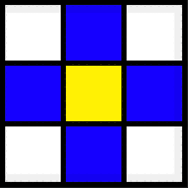
\includegraphics[width=.6\linewidth]{Section1/1}
   	\end{subfigure}\hfill
   	\begin{subfigure}{0.48\textwidth}
     		\centering
     		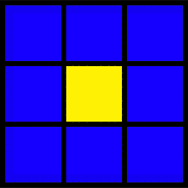
\includegraphics[width=.6\linewidth]{Section1/2}
   	\end{subfigure}
   	\caption[Neighborhood configuration]{The von Neumann neighborhood (on the left) includes the surrounding four cells of the center cell. The Moore neighborhood (on the right) includes the surrounding eight cells of the center cell.}
   	\vspace{-1.5em}
   	\label{fig:Neighborhood configuration}
\end{figure}

Since there are two possible states in the Game of Life, the live cells satisfying the survival rule and the dead cells satisfying the born rule will be alive in the next generation, and the remaining cells will all be dead. The probability of surviving and being born is $\frac{2}{9}$ and $\frac{1}{9}$ respectively. The evolution rule is often visualized using cellular automaton state transition diagrams, where each vertex on the graph represents one of the states and each directed edge represents a viable evolution from one state to another. The probability of that transition, if available, will be highlighted on the edge. Figure ~\ref{fig:Transitional state diagram of the Game of Life} shows the transitional state diagram of the Game of Life. 

\begin{figure}[H]
	\centering
	
\includegraphics[width=\linewidth]{Section1/3}
	\caption[Transitional state diagram of the Game of Life]{Transitional state diagram of the Game of Life. The probability of the transition followed by the specific satisfying state requirements in parentheses is highlighted on the corresponding edge. For example, the edge connecting the dead state to the live state represents the action of a cell being born. The probability of being born is $\frac{1}{9}$. Specifically, a dead cell needs three live cells in its neighborhood to be born.}
	\label{fig:Transitional state diagram of the Game of Life}
	\vspace{-1.5em}
\end{figure}

Cellular automata become much more complicated and interesting when there are more than two possible states. In this case, apart from the live (i.e, healthy) and dead cells, there are also transitional dying cells (i.e., sick cells) in between and we are free to implement new rules to define how all of these states transition to other states. In the rest of the report, healthy and live cells refer to the same thing and are thus used interchangeably. These newly added rules, combined with the survival and born rules, constitute a new set of evolution rules. 

Some of the most frequent patterns generated by the rules are “still life”, which are static patterns that do not change between generations, and “oscillators”, which are periodic patterns that return to their initial state after a finite number of generations \cite{Cellular automaton}. While these patterns are fun, the feature that makes the Game of Life so well-known is undoubtedly the discovery of “gliders” \cite{Glider}. \textit{Gliders}, also known as translating oscillators, “spaceships” or “fish”, are automata that travel by looping through a short series of iterations and end up in a new location after each cycle returns to the original configuration \cite{rake}. They are usually considered the most interesting pattern and are widely used for modeling complicated nonlinear systems in computational science, physics, chemistry, and biology \cite{Cellular automaton}. If we think of cellular automata as an ecosystem, then the gliders are a unique kind of independent life form within. Finding gliders can potentially help us answer questions like how accurately we are simulating biological life, or whether our artificial life forms can adapt to a changing environment. 

\textit{Period} and \textit{speed} are the two frequently-utilized metrics to describe a glider. Period refers to the number of ticks a pattern must iterate through before returning to its initial configuration \cite{The Game of Life}. The speed of the glider is expressed in terms of the metaphorical “speed of light”, $c$ \cite{spaceship, speed of light}. The speed of light is a propagation rate across the grid of exactly one step, either horizontally, vertically, or diagonally, per generation. Since a cell can only influence its nearest neighbors, the speed of light is the upper bound to the speed at which any pattern can move. Generally, if the glider in a two-dimensional automaton is translated by $(x,y)$ after $n$ generations, then the speed $v$ is defined as: 
$$v = \frac{\max{(|x|, |y|)}}{n}c$$
The most famous glider found by Conway is the first one in Figure ~\ref{fig:GOL examples} with a period of 4 and a speed of $\frac{c}{4}$, as it takes four generations for a given state to be translated by one cell diagonally. There are many other cellular automata rules besides the Game of Life that can produce gliders. Figure ~\ref{fig:famous gliders} shows some of the famous gliders and \textit{glider generators}, a pattern with a main part that repeats periodically, like an oscillator, and that also periodically emits gliders \cite{gun}, that have been generated with other sets of rules featured in Cellular Automata Rules Lexicon \cite{Lexicon}. 

\begin{figure}[H]
	\centering
  	\begin{subfigure}{0.18\textwidth}
     		\centering
     		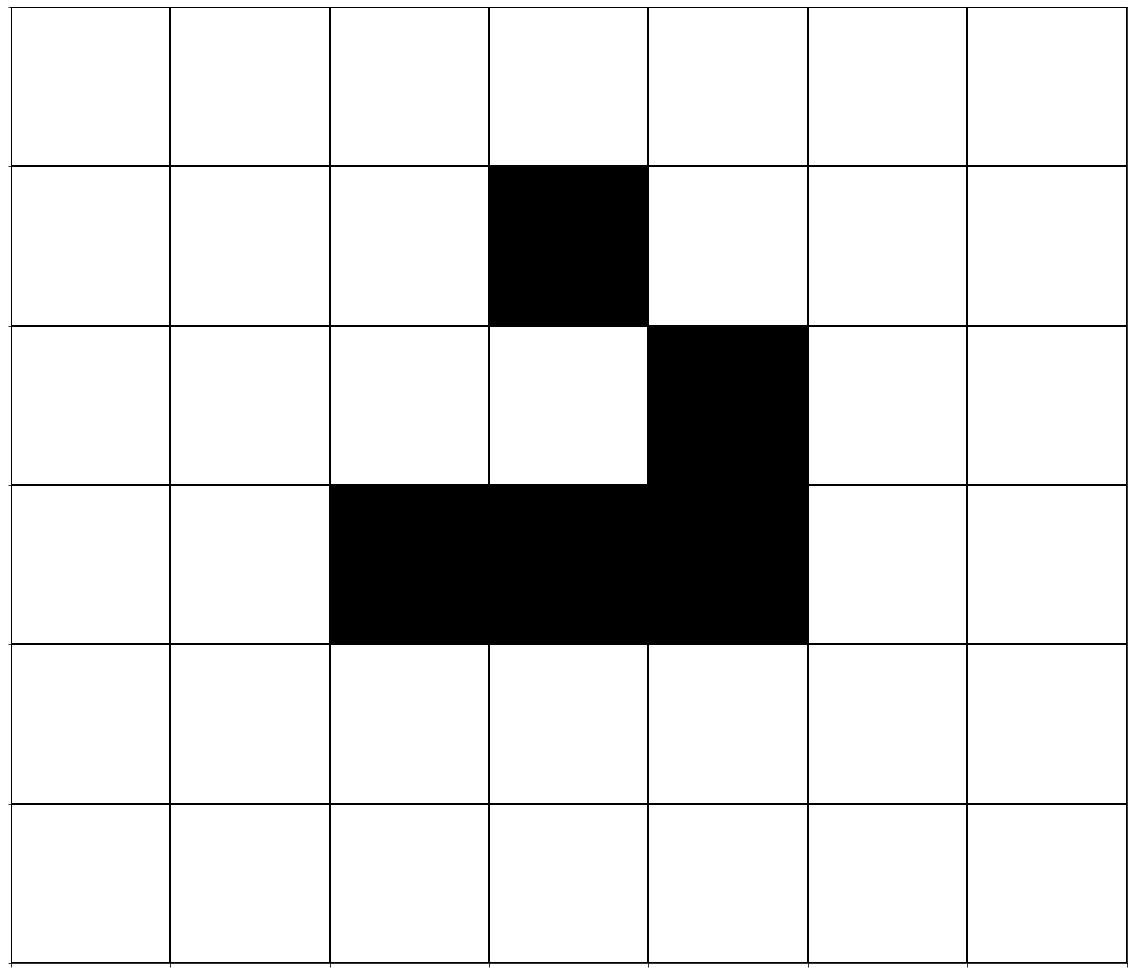
\includegraphics[width=\linewidth]{Section1/4.0}
     		\subcaption{}
   	\end{subfigure}
     	\begin{subfigure}{0.18\textwidth}
     		\centering
     		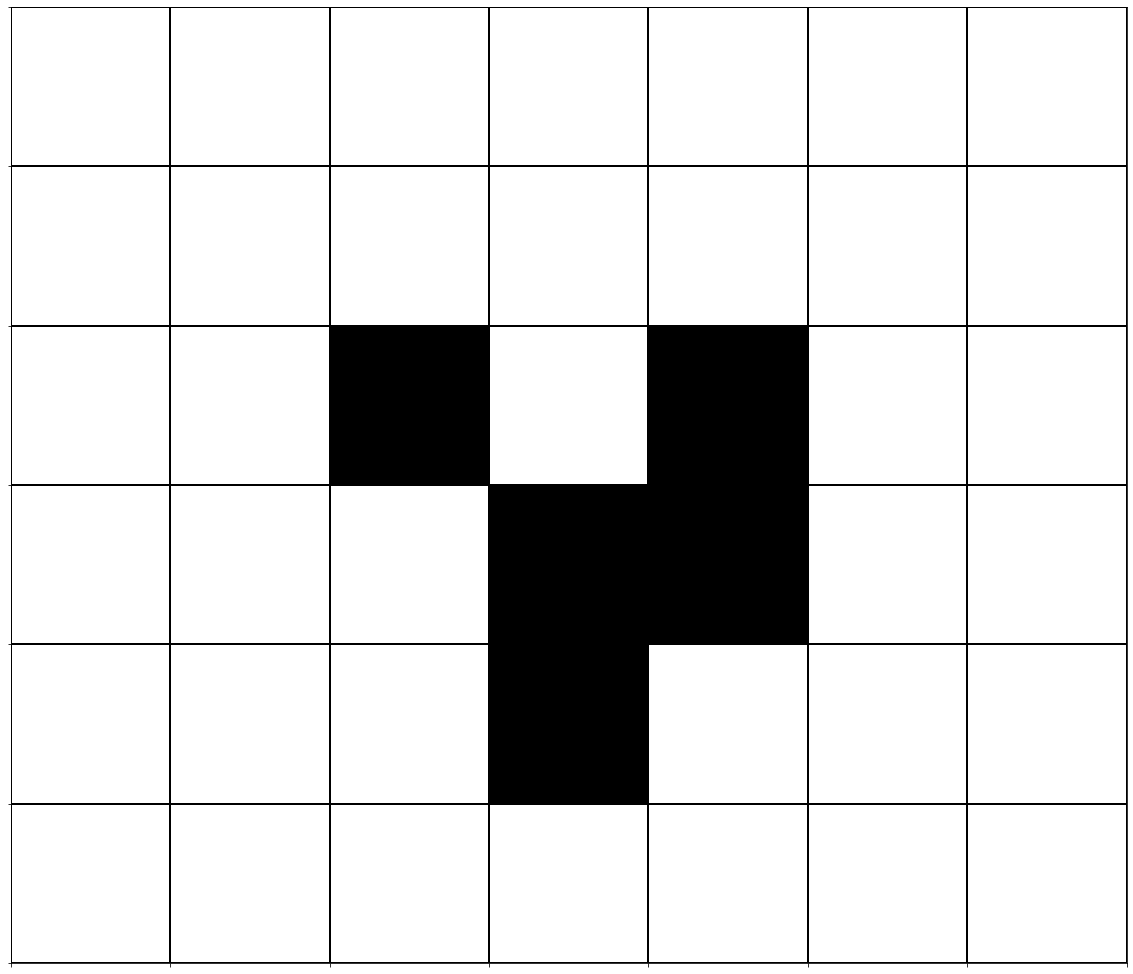
\includegraphics[width=\linewidth]{Section1/4.1}
     		\subcaption{}
   	\end{subfigure}
     	\begin{subfigure}{0.18\textwidth}
     		\centering
     		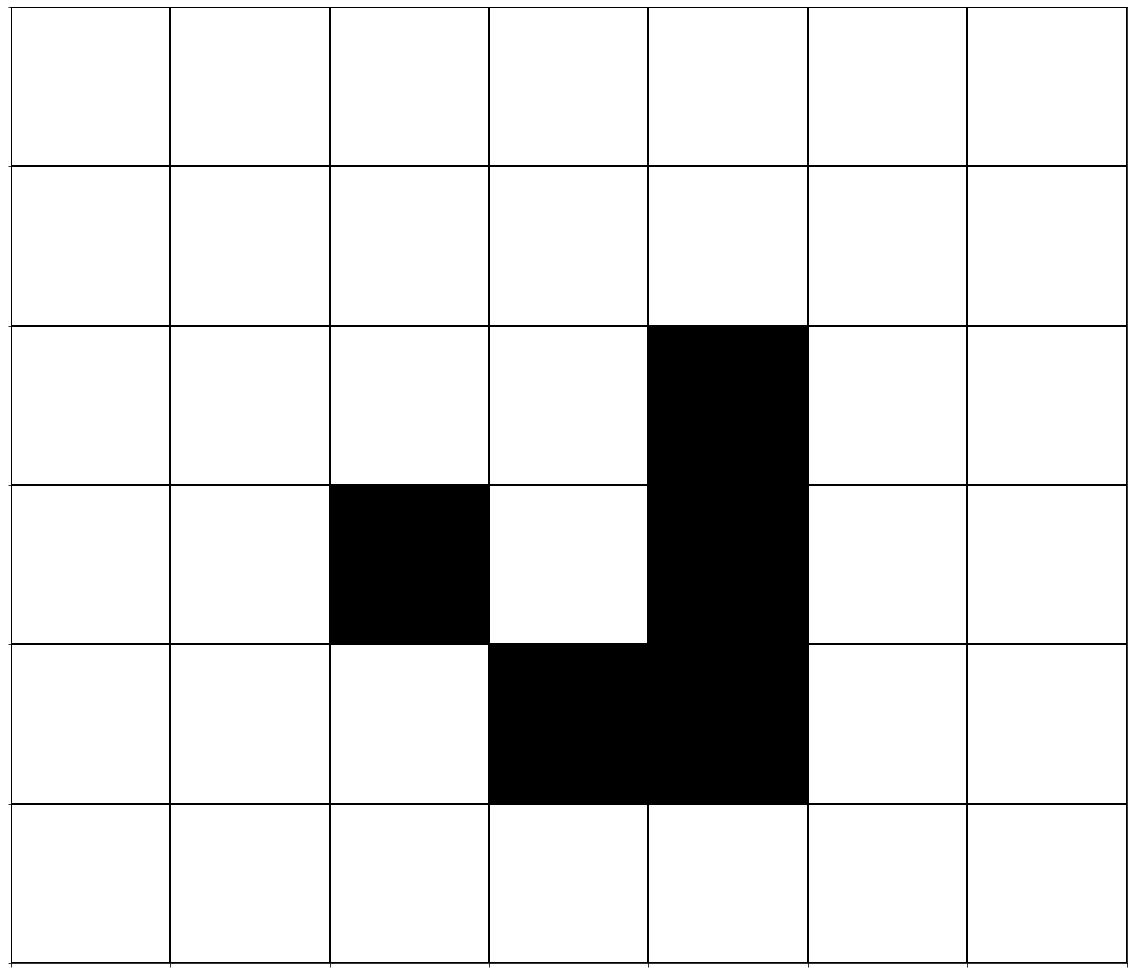
\includegraphics[width=\linewidth]{Section1/4.2}
     		\subcaption{}
   	\end{subfigure}
    	\begin{subfigure}{0.18\textwidth}
     		\centering
     		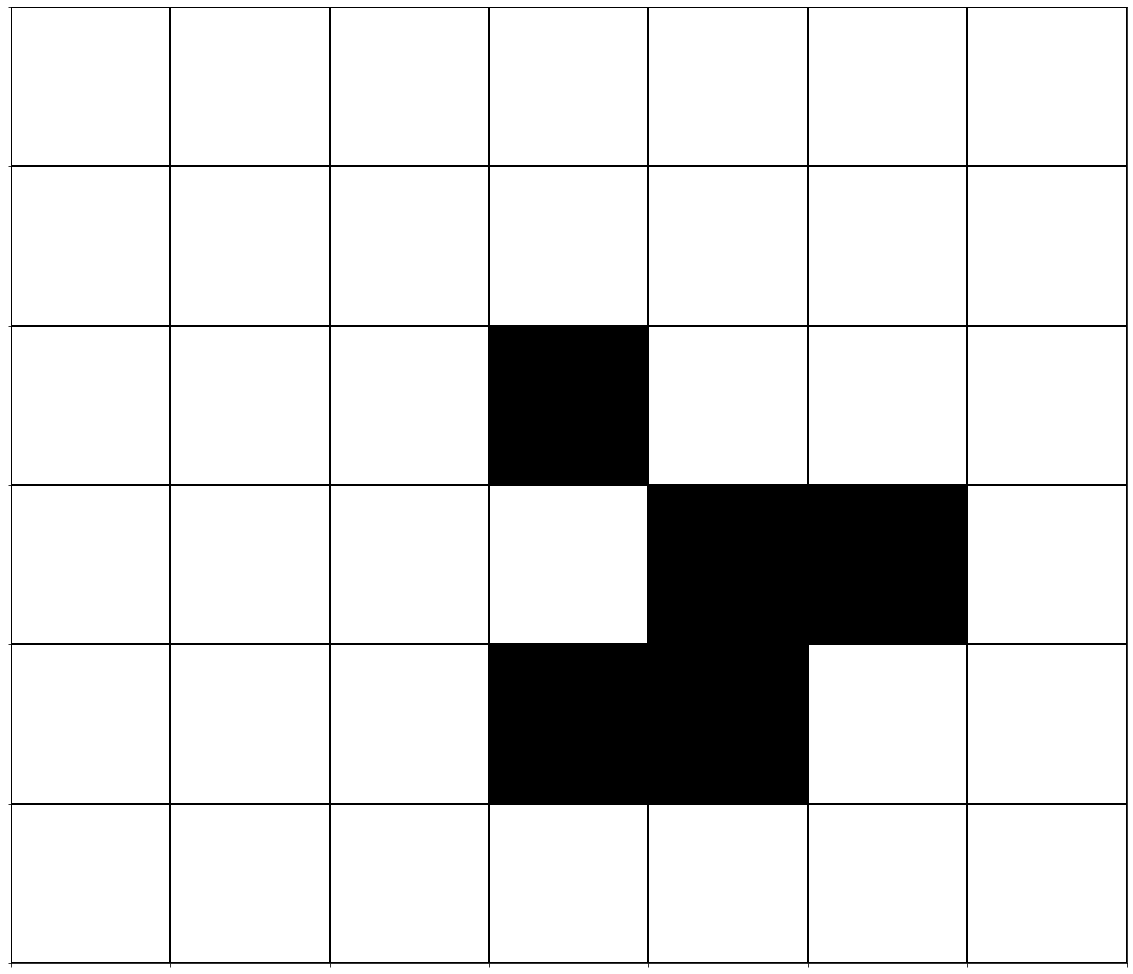
\includegraphics[width=\linewidth]{Section1/4.3}
     		\subcaption{}
   	\end{subfigure}
   	\begin{subfigure}{0.18\textwidth}
     		\centering
     		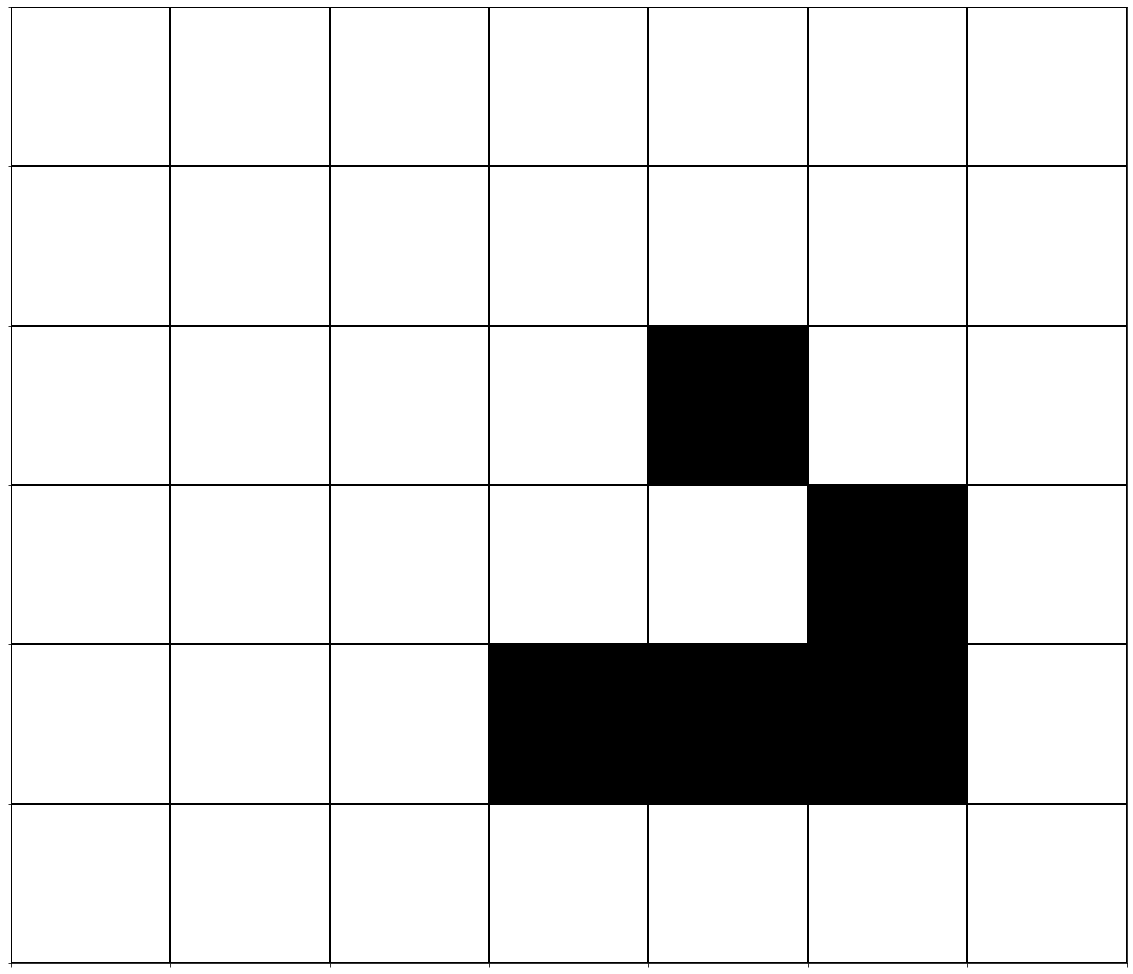
\includegraphics[width=\linewidth]{Section1/4.4}
     		\subcaption{}
   	\end{subfigure}
   	{\LARGE$\searrow{}$}
   	\setcounter{subfigure}{0}
	\centering
  	\begin{subfigure}{0.18\textwidth}
     		\centering
     		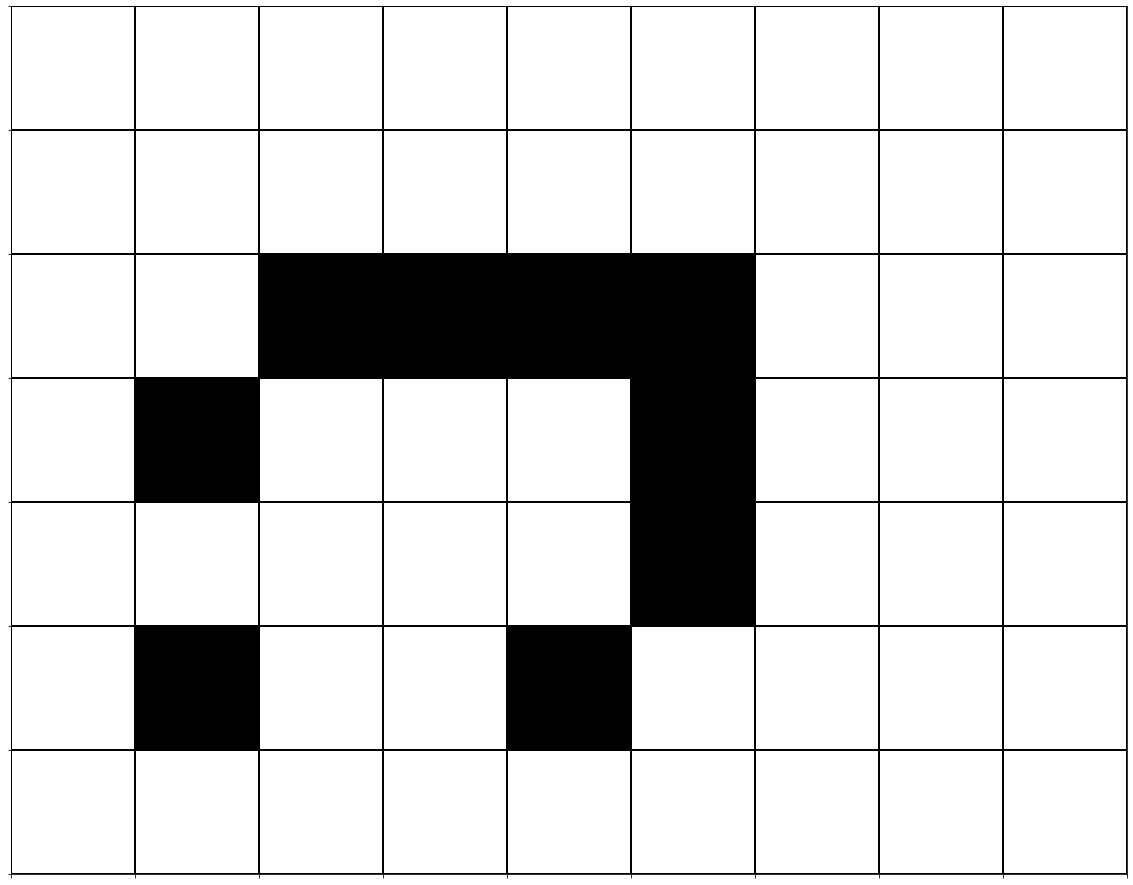
\includegraphics[width=\linewidth]{Section1/5.0}
     		\subcaption{}
   	\end{subfigure}
     	\begin{subfigure}{0.18\textwidth}
     		\centering
     		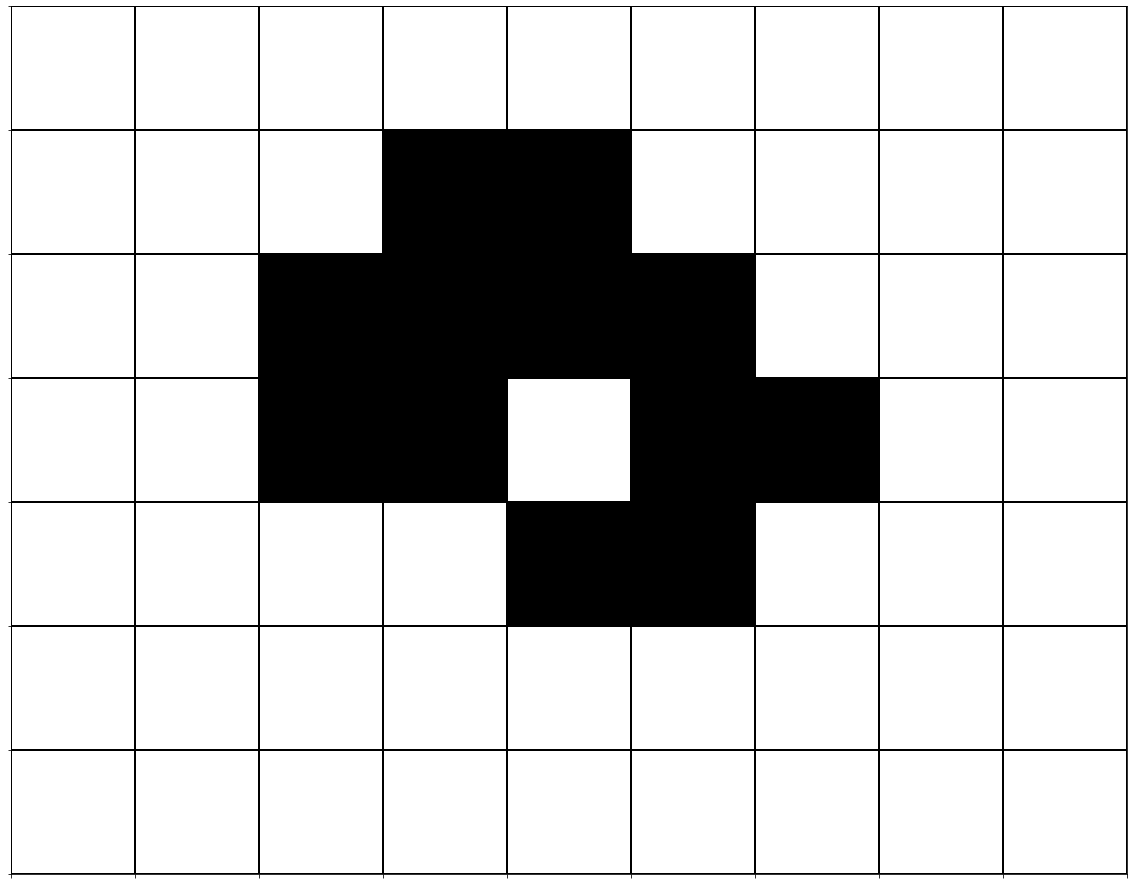
\includegraphics[width=\linewidth]{Section1/5.1}
     		\subcaption{}
   	\end{subfigure}
     	\begin{subfigure}{0.18\textwidth}
     		\centering
     		
\includegraphics[width=\linewidth]{Section1/5.2}
     		\subcaption{}
   	\end{subfigure}
     	\begin{subfigure}{0.18\textwidth}
     	\centering
     		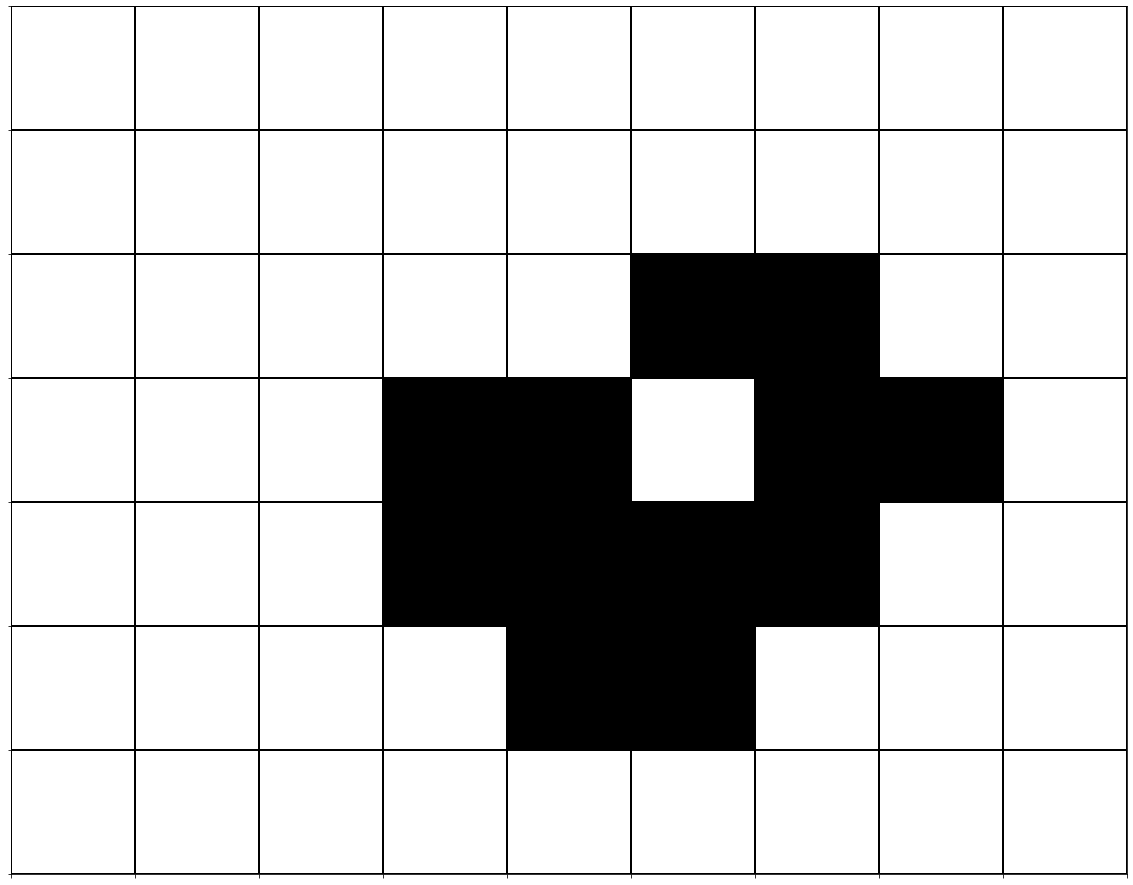
\includegraphics[width=\linewidth]{Section1/5.3}
     		\subcaption{}
   	\end{subfigure}
   	\begin{subfigure}{0.18\textwidth}
     		\centering
     		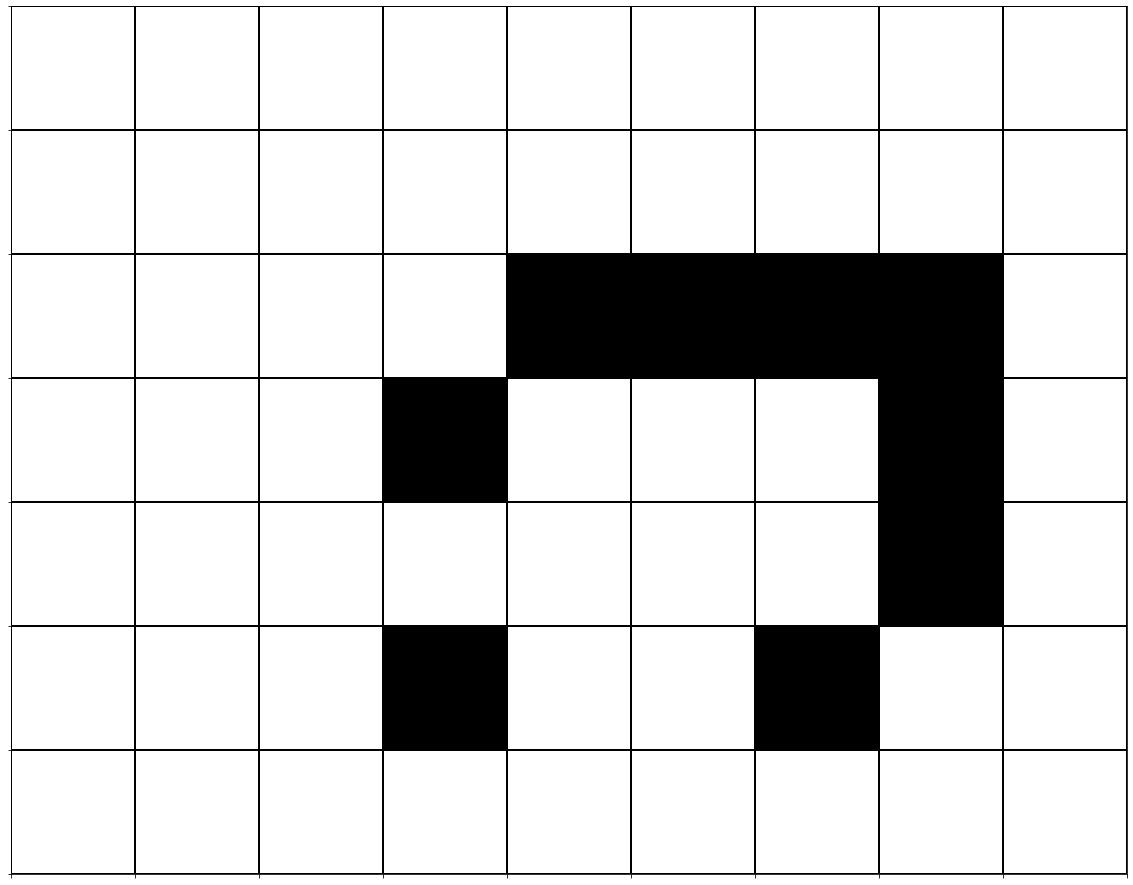
\includegraphics[width=\linewidth]{Section1/5.4}
     		\subcaption{}
   	\end{subfigure}
   	{\LARGE$\rightarrow{}$}
	\setcounter{subfigure}{0}
	\centering
 	\begin{subfigure}{0.18\textwidth}
     		\centering
     		
\includegraphics[width=\linewidth]{Section1/6.0}
     		\subcaption{}
   	\end{subfigure}
    	\begin{subfigure}{0.18\textwidth}
     		\centering
     		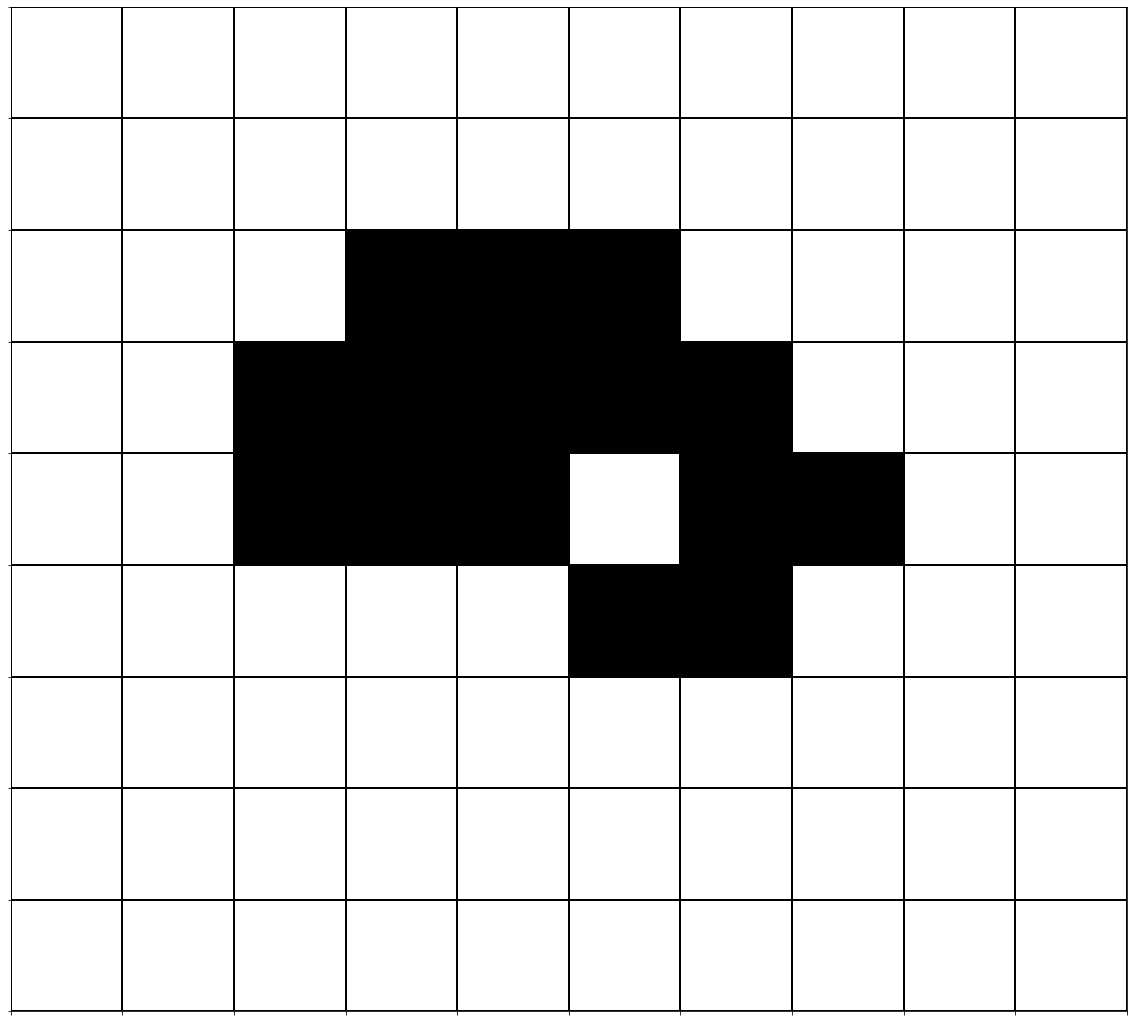
\includegraphics[width=\linewidth]{Section1/6.1}
     		\subcaption{}
   	\end{subfigure}
     	\begin{subfigure}{0.18\textwidth}
     		\centering
     		
\includegraphics[width=\linewidth]{Section1/6.2}
     		\subcaption{}
   	\end{subfigure}
     	\begin{subfigure}{0.18\textwidth}
     		\centering
     		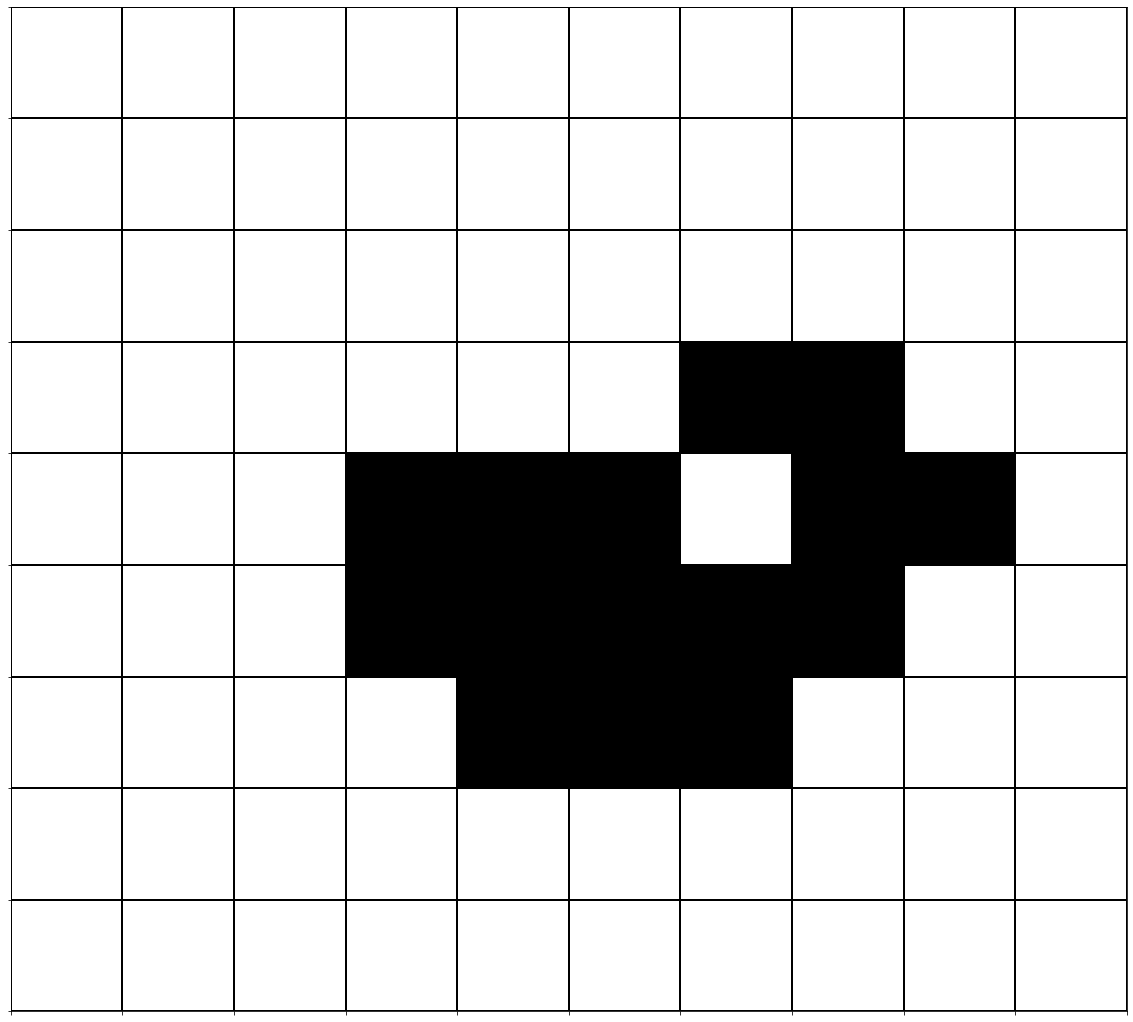
\includegraphics[width=\linewidth]{Section1/6.3}
     		\subcaption{}
   	\end{subfigure}
   	\begin{subfigure}{0.18\textwidth}
     		\centering
     		
\includegraphics[width=\linewidth]{Section1/6.4}
     		\subcaption{}
   	\end{subfigure}
   	{\LARGE$\xrightarrow{}$}
%\end{figure}
	\setcounter{subfigure}{0}
%\begin{figure}[H]
	\centering
  	\begin{subfigure}{0.18\textwidth}
     		\centering
     		
\includegraphics[width=\linewidth]{Section1/7.0}
     		\subcaption{}
   	\end{subfigure}
     	\begin{subfigure}{0.18\textwidth}
    		\centering
     		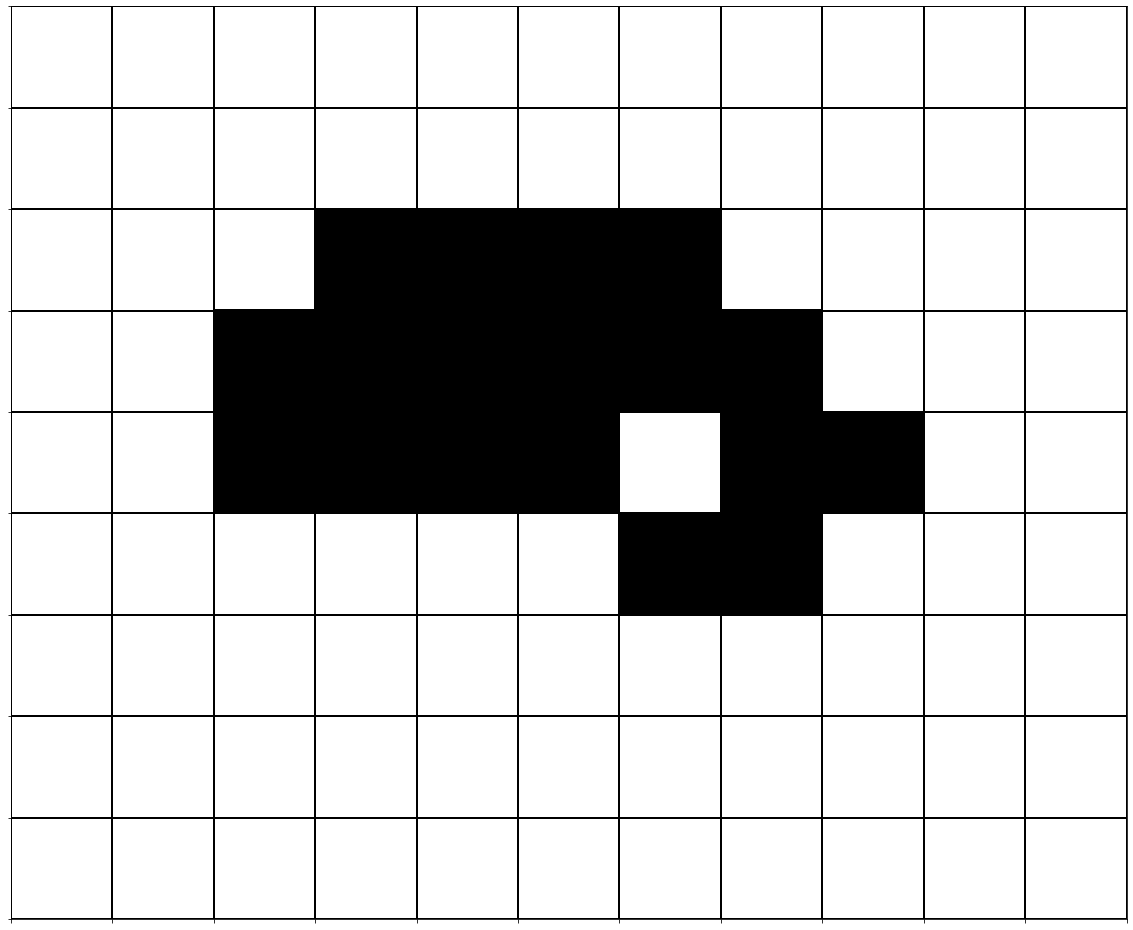
\includegraphics[width=\linewidth]{Section1/7.1}
     		\subcaption{}
   	\end{subfigure}
     	\begin{subfigure}{0.18\textwidth}
     		\centering
     		
\includegraphics[width=\linewidth]{Section1/7.2}
     		\subcaption{}
   	\end{subfigure}
    	\begin{subfigure}{0.18\textwidth}
     		\centering
     		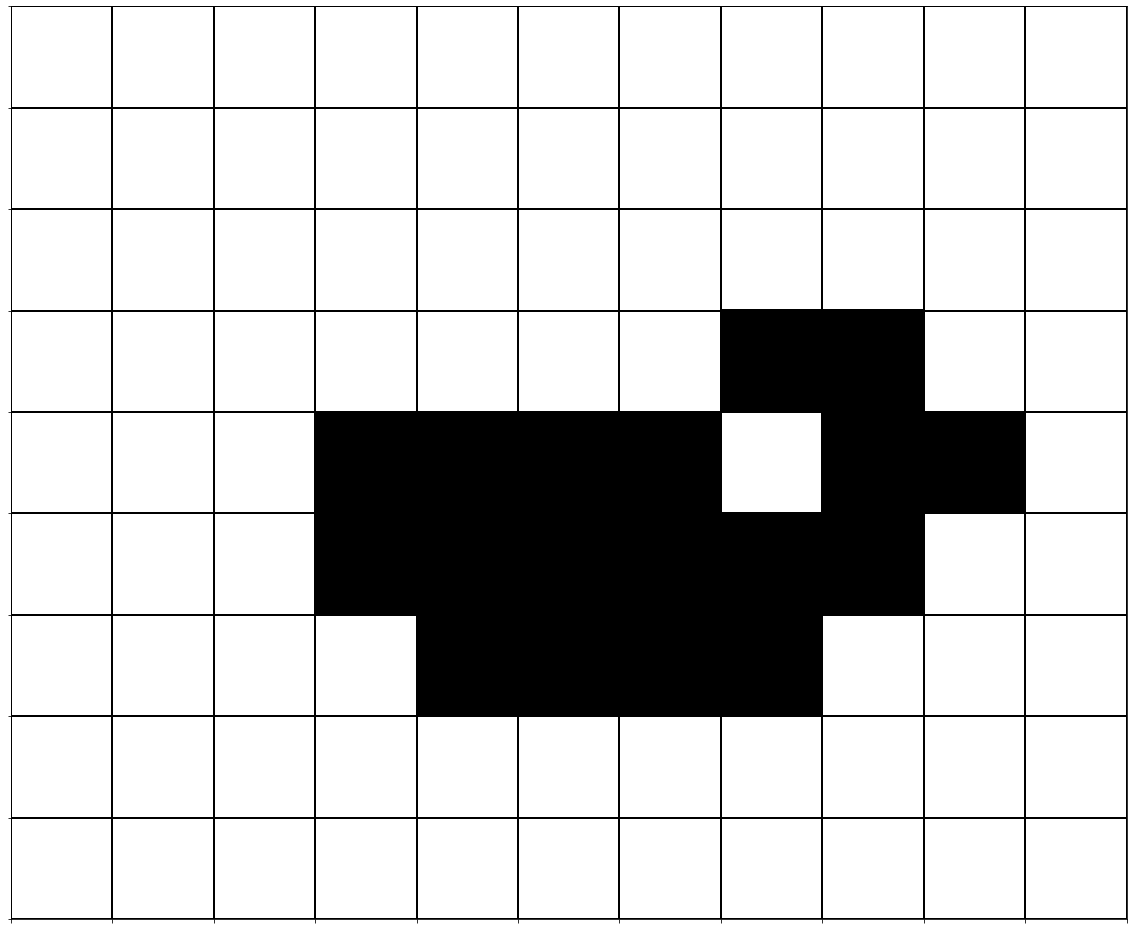
\includegraphics[width=\linewidth]{Section1/7.3}
     		\subcaption{}
   	\end{subfigure}
   	\begin{subfigure}{0.18\textwidth}
     		\centering
     		
\includegraphics[width=\linewidth]{Section1/7.4}
     		\subcaption{}
   	\end{subfigure}
   	{\LARGE$\xrightarrow{}$}
	\caption[Gliders in the Game of Life]{Gliders generated by the Game of Life “2,3/3/2” rule. The top is the original glider first found by Conway. The rest are the light-weight, mid-weight and heavy-weight spaceships respectively. All four gliders have a period of four. The light-weight, mid-weight and heavy-weight spaceship have a speed of $\frac{c}{2}$, as it takes four generations for a given state to be translated by two cells. Code is provided in ~\ref{subsubsection:GOL}, ~\ref{subsubsection:lightweight spaceship}, ~\ref{subsubsection:midweight spaceship}, ~\ref{subsubsection:heavyweight spaceship}.}
	\label{fig:GOL examples}
	\vspace{-1.5em}
\end{figure}

\begin{figure}[H]
	\begin{subfigure}{0.45\textwidth}
     		\centering
     		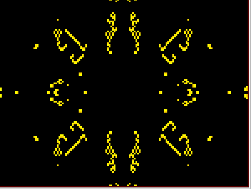
\includegraphics[width=\linewidth]{Section1/8.1}
     		\subcaption{}
   	\end{subfigure}
     	\begin{subfigure}{0.53\textwidth}
     		\centering
     		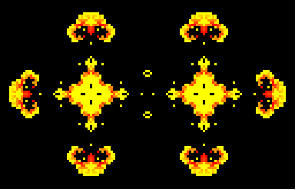
\includegraphics[width=\linewidth]{Section1/8.2}
     		\subcaption{}
   	\end{subfigure}
     	\begin{subfigure}{0.42\textwidth}
     		\centering
     		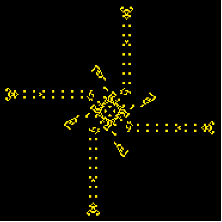
\includegraphics[width=\linewidth]{Section1/8.3}
     		\subcaption{}
   	\end{subfigure}
     	\begin{subfigure}{0.56\textwidth}
     	\centering
     		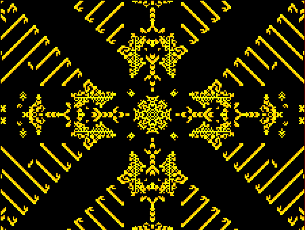
\includegraphics[width=\linewidth]{Section1/8.4}
     		\subcaption{}
   	\end{subfigure}
   	\caption[Examples of famous gliders]{Four examples of discovered glider generators with different rules. They are "Brian’s Brain" with rule “/2/3” (top left), "Burst" with rule “0,2,3,5,6,7,8/3,4,6,8/9” (top right), "Brain6" with rule “6/2,4,6/3” (bottom left), and "Star Wars" with rule “3,4,5/2/4” (bottom right) \cite{Lexicon}.}
   	\label{fig:famous gliders}
   	\vspace{-1.5em}
\end{figure}

The gliders in Figure ~\ref{fig:famous gliders} belong to the category of outer totalistic generations of two-dimensional cellular automata and are generated using the Moore neighborhood with decay. In other words, it uses the “Instant birth, gradual death, no recovery” model depicted in Figure ~\ref{fig:IGN model}. 

\begin{figure}[H]
	\centering
	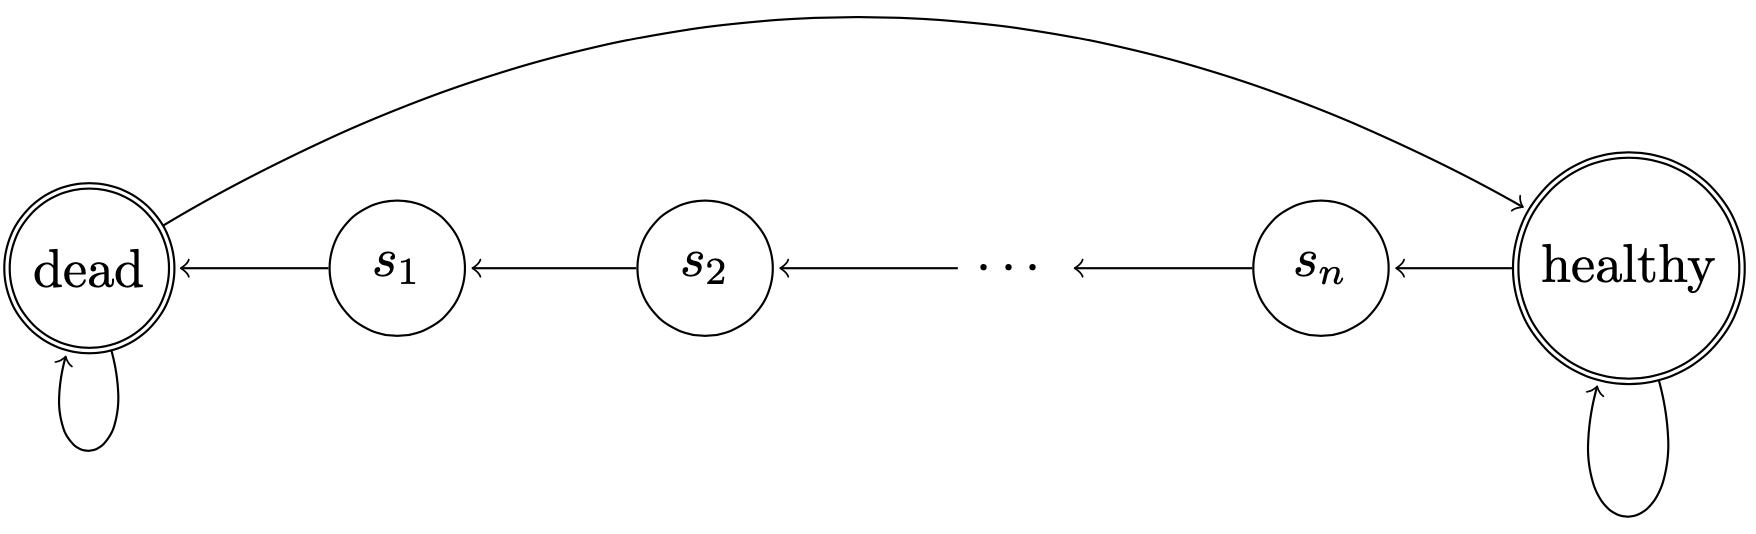
\includegraphics[width=\linewidth]{Section1/9}
	\caption["Instant birth, gradual death, no recovery” Model]{"Instant birth, gradual death, no recovery” Model. Healthy cells can get sick. Sick cells are not able to recover, and they will be one step closer to death at each step. Dead cells cannot be born sick.}
	\label{fig:IGN model}
	\vspace{-1.5em}
\end{figure}

The behavior of sick cells under this model is deterministic as they are not able to recover and can only approach one step closer to death at each step. The healthy cells that do not satisfy the survival rule will become sick and inevitably enter the path of gradual death. Hence, we do not need extra parameters to categorize the behavior of sick cells. Specifically, like the Game of Life,  three parameters constitute the rules of the model: 
\begin{enumerate}[topsep=0pt,itemsep=-1ex,partopsep=1ex,parsep=1ex]
\item The number of total possible states. 
\item The survival rule that determines which of the live cells survive in the next step. 
\item The born rule that determines which of the dead cells are born in the next step. 
\end{enumerate}
The canonical way to represent the evolution rules of the generations is “S/B/C”, where S, B, and C represents the survival rule, the born rule, and the count of states cells can have respectively \cite{Lexicon}. Hence, the Game of Life can be summarized as the “2,3/3/2” rule.

Not all rules are able to produce beautiful results like the ones in Figure ~\ref{fig:famous gliders}. In fact, the results from most of the rules turn out to be unappealing. Configurations under some rules always die out, while others might lead to explosive growth. It is worth noting that gliders exist for many unstable rules, especially those that lead to explosive growth. However, in this case, there is no real value in exploring them because they often disappear quickly and move around recklessly without clear patterns. Therefore, we shall only consider gliders for stable rules that exhibit bounded growth and eventually yield a finite number of gilders. One potential problem is that there may be some carefully constructed initial configuration within an interesting rule that could lead to explosive growth or stasis \cite{Gliders in Cellular Automata}. However, statistically it has an extremely low probability if the initial configuration is randomly generated. In this report, we decided to define the rules that satisfy these requirements using the “Instant birth, gradual death, no recovery” model with the Moore neighborhood as interesting. Specifically, the definition of \textit{interesting rules} in this report includes: 
\begin{enumerate}[topsep=0pt,itemsep=-1ex,partopsep=1ex,parsep=1ex]
\item It uses the Moore neighborhood. 
\item It uses the “Instant birth, gradual death, no recovery” model, which means the evolution rule consists of the survival rule, the born rule, and the number of possible states. 
\item Random initial configurations will always eventually stabilize (i.e., non-static and non-explosive). 
\item It produces a finite number of gliders. 
\end{enumerate}

All the remaining rules in the same model that lead to stasis, noise with no discernible patterns moving across the screens, or some patterns other than gliders, are classified as boring. Finding out what the interesting rules are and what the gliders look like is a daunting task. Under most circumstances, it is impossible to tell whether the rule is interesting or boring just by looking at the parameters of the rules. Furthermore, in one single case where we have a total of 10 possible states (i.e., 8 sick states), there are $2^9$ survival rules and $2^9$ born rules, which already leads to a total of $2^{18}$ combinations of rules. Given the fact that we may also want to explore rules with other number of total states, this eventually becomes an impossible task with normal computer software. Because of this daunting number of possibilities, automatic detection of interesting rules will be very helpful, so that users do not have to manually go through the process. 

This report explores the possibility of using deep neural networks to detect these interesting cellular automata rules. Deep neural networks, a branch of machine learning, are computational algorithms that can extract information from complicated data to detect patterns or trends which are too convoluted for human brains and other computer software. The most unique property of neural networks is that once trained, they can learn and adapt to new situations on their own. In this way, their learning process resembles the cognitive development of the human brain, which is made of neurons, the fundamental building unit for information transmission. These characteristics make neural networks much better candidates than humans to distinguish the interesting rules in cellular automata. We will train the neural network on a dataset consisting of samples of interesting and boring rules so that the machine learner can gradually recognize the decisive properties that distinguish interesting from boring rules. After the training, validating, and testing processes, our machine learner would be ready to dive into the remaining search space of rules that have not yet been classified and collect the interesting ones. The best part about it is that humans do not need to be involved in the exploration process at all, which is the most tedious and time-consuming step. All we have to do is manually inspect the rules that have been classified as interesting by our machine learner and record the gliders within the patterns if they have been classified correctly. 

Specifically, we first built the dataset from scratch by programming the generation algorithm and applying data augmentation to selected known rules. Then we used Recurrent Neural Networks (RNN), Convolutional Neural Networks (CNN), feature extraction, entropy analysis, and other techniques to help find interesting rules that generate gliders. We then put the trained machine learners into practice and detected several new rules with only three states. We discovered an entire \textit{family} of gliders of different periods, Frankenstein gliders, the new Life, and many other interesting results.

\newpage
\section{Related Work}
\label{Related Work}
John Conway, regarded as the father of cellular automata and the “founder of life”, first described this elegant mathematical model of computation in 1970. From his famous rules of Game of Life emerged a five-celled organism that moves diagonally across the grid. This discovery has attracted a group of fanatics who dedicated themselves to constructing rules in hopes of spotting new life forms. However, there has not been a systematic method of identifying interesting rules and the progress of searching has been rather slow. 

The hype for cellular automata reached its peak when Stephen Wolfram published “A New Kind of Science” in 2002, which is also regarded as the encyclopedia of cellular automata \cite{A new kind of Science}. In the book, he introduced a large variety of cellular automata with many arbitrary rules that generate interesting results. However, the most important lesson from his book is that complexity arises from simplicity and there is incredible richness in the computational universe. Even the simplest rule can produce the most complicated and unpredictable behavior. The vast space of the computational universe and the scarcity of the discovered rules gives us the potential to mine the interesting rules and harness them for our purposes. Wolfram describes the process of looking for something interesting in the space of cellular automata as very different from our accustomed approach of building models step by step while ensuring that we have control over their behaviors. He makes the rather counterintuitive claim that we should not try building anything at all. Instead, we should just define what we want and then search for it in the computational universe. It is sometimes very easy and fast to find what we want. For example, Wolfram quickly came across with rule 30 \cite{Rule 30} in Figure ~\ref{fig:Rule 30}, which is a one-dimensional cellular automata rule with two states and later became one of the best-known generators of apparent randomness, just by enumerating the rules. However, in other cases, it might take much longer, like it took Wolfram millions of attempts to find the simplest universal Turing machine. 
 
\begin{figure}[H]
	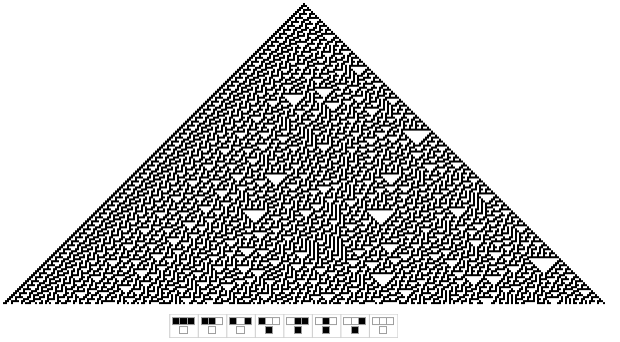
\includegraphics[width=\linewidth]{Section2/1}
	\caption[Wolfram's Rule 30]{Wolfram’s Rule 30 \cite{Rule 30}.}
	\vspace{-1.5em}
	\label{fig:Rule 30}
\end{figure}

The justification he makes for his claim is that when one looks at what the cellular automata is doing, one does not comprehend how it really works. Just like nature, one might be able to analyze some of its parts and be impressed with how smart they are, but it would be extremely hard to understand the full picture. Wolfram claims by the laws of computational irreducibility that we had to do an irreducible number of computations to figure out precisely what the generated patterns look like. In other words, there are no shortcuts and the only viable method is to do a full-sized simulation. Therefore, it is radically different from exact science where we normally predict the behaviors of the models by solving mathematical equations. Hence, it is in vain to even attempt to manipulate or systematically build a cellular automata rule which generates the desired pattern. 

Nevertheless, despite the unpredictable nature of cellular automata, there have been some approaches to find interesting two-dimensional cellular automata rules containing gliders. The most naïve is to repeatedly create random neighborhood rules and inspect if it generates an interesting result. This method only works for lower dimensional cellular automata (specifically one-dimension), whose parameter search space is relatively small. In this case, we can brute force all the possible sets of rules and manually inspect which ones are interesting after the generations are saved. However, when it comes to higher-dimensional cellular automata, even a two-dimensional one, the parameter search space becomes gigantic, and most rules would not produce gliders. Hence, this method becomes inefficient and random as the experiment turns into a pure matter of luck. Another approach is to make slight modifications to known interesting rules, such as John Conway’s the Game of Life, to generate similar or refined patterns. This specifically involves modifying one or two of the parameters while leaving the rest unchanged. However, this practice usually leads to a radically different result than the original because the interesting rules are not necessarily clustered together in the parameter search space. Consequently, this method turns out to be not much more promising than the first. Nevertheless, despite their randomness and ineffectiveness, the two methods mentioned above are commonly used to find rules containing gliders. 

A more systematic method to find gliders is introduced by Andrew Wuensche in Collision-Based Computing \cite{Finding Gliders in Cellular Automata}. He proposed that this could be achieved by a measure of the variance of input entropy over time. The distribution of rule classes in rule-space is discovered. The method also allows automatic “filtering” of cellular automata space-time patterns to show up gliders and related emergent configurations more clearly. Cellular automata dynamics are shown to exhibit some approximate correlations with global measures on convergence in attractor basins, characterized by the distribution of in-degree sizes in their branching structure, and to the rule parameter Z. 

There are also some computational methods to determine the type of the generated cellular automata. For example, Christopher Langton created a cellular automata lambda value that is computed based on the number of cells that have been born at that time step and dividing it by the total number of cellular automata cells \cite{Edge of Chaos}. This formula generates a decimal value between 0 and 1. The endpoints of the interval, 0 and 1, correspond to the static patterns and explosive growth respectively. Based on his classification, a lambda value within 0.1 and 0.15 indicates an interesting rule that requires further investigation. However, the most well-known classification of cellular automata is introduced by Stephen Wolfram, which consists of four different classes: automata in which patterns stabilize into homogeneity, automata in which patterns evolve into mostly stable or oscillating structures, automata in which patterns evolve into chaos, and automata in which patterns become extremely complex \cite{Cellular automaton}. Based on his classification, the fourth class is potentially computational universal and worth investigating. But neither Langton nor Wolfram established a connection between the classifications and the rules themselves.  

None of these described methods have been proven to be reliable as they usually find noise or stasis. Therefore, detecting gliders in two-dimensional outer totalistic cellular automata is an unsolved problem and this report will introduce the potential of neural networks to detect interesting rules. The main idea is that we will build machine learners, which are much more computationally capable than humans and other programs, to help determine whether the rules would be interesting. If we think of the parameter space as an ocean, then an interesting rule is like a particular depth and the gliders are the fish at that depth. Instead of randomly choosing a depth and inspect whether fish can survive, we can quickly scan a vast volume of the sea and inspect those depths that have fish swimming in it. Given sufficient computers and memory, we have the potential to detect all the interesting rules containing gliders. 

Interestingly, Wolfram also described an uncanny systematic resemblance between neural networks and cellular automata in his book \cite{A new kind of Science}. The parameters in neural networks are never explicitly set or engineered but are generated automatically. Similar things happen with cellular automata as the patterns are never artificially constructed. What differentiates between the two is that in neural networks there are learning processes, where the weights are improving according to rules of linear algebra and calculus. However, in cellular automata, the parameters of the rules are not necessarily improving, and one is forced to enumerate all possibilities.

\newpage
\section{Methodology}
\label{Methodology}
We first collected the two-dimensional cellular automata data that the machine learner could use for training, validation, and testing. This entailed designing and implementing a data-collection pipeline from scratch to generate a sequence of raw frames for each of the patterns. Then we tested several models and analyzed for the best results. We trained the data with different models including RNN and CNN, and performed hyperparameter tuning, image feature extraction, and entropy analysis. 

\subsection{Dataset Generation}
The foremost step was to program the cellular automata evolution algorithm, which computes the states of each cell in the next generation based on the rules and the current configuration. The logic follows the rules in the “Instant birth, gradual death, no recovery” model: in the next generation, the live cells that satisfy the survival rule and the dead cells that satisfy the born rule will be alive, the live cells that do not satisfy the survival rule will become sick, the cells that are in the dying transitional (sick) states will move one step closer to death, and the remaining dead cells that do not satisfy the born rule will remain dead. The survival rule, born rule, the total number of possible states, and the neighborhood were passed in as parameters. The specific implementation of the algorithm can be found in ~\ref{subsection:Cellular Automata Generation Algorithm}. 

We were able to keep track of the evolution of all cells in the grid in each generation using the evolution algorithm. With the help of $CellPyLib$, which is a python package supporting the visualization of two-dimensional, k-color, adjustable neighbor cellular automata, we could save the evolution as a sequence of frames. However, we still needed to collect known rules so that we could pass them into the algorithm and train our machine learner on the generated sequence of frames later. To obtain boring rules, we manually went through random examples and collected those that died out immediately, generated static noise or boring non-glider patterns. Enumeration proved to be quite effective because most rules fall under the category of boring, and we easily collected 105 boring rules using this method. Interesting rules, on the other hand, are more rare, and thus were harder to find. Hence, we borrowed existing examples provided in Cellular Automata Rules Lexicon and recorded those with gliders. Eventually, we successfully collected 35 rules that can be subjectively classified as interesting. The set of interesting rules we included in our dataset is described in ~\ref{subsection:The 35 Selected Interesting Rules}. 

Because of the limited number of rules that we classified, we decided to apply data augmentation to increase the size of the dataset to a reasonable size exceeding 1,000. Since we also wanted to maintain a 50/50 split of the two patterns for training purposes, we reused each boring and interesting rule 10 and 30 times with different random initial configurations. Consequently, we generated a total of 1050 boring and 1050 interesting patterns. For each of the patterns, we recorded 140 consecutive generations as grayscale frames using $CellPyLib$, which was usually more than enough for the patterns to stabilize. The living and dead cells were in black and white respectively. The remaining sick cells were assigned with a grayscale color in between depending on their specific state. Figure ~\ref{fig:generated frame example} shows an example of a generated frame. This happened to be the most time-consuming step as it took roughly five hours to go through the lexicons and record the interesting ones, and another 12 hours to generate the frames. 

\begin{figure}[H]
	\centering
	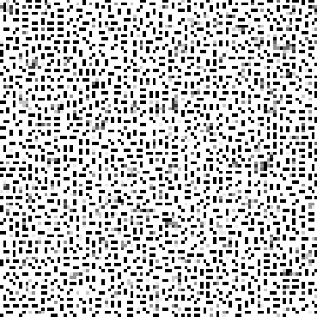
\includegraphics[width=0.5\linewidth]{Section3/1}
	\caption[Example of a generated frame]{Frame 107 of a boring rule “1,5,8/2/7” with a random initial configuration.}
	\vspace{-1.5em}
	\label{fig:generated frame example}
\end{figure}

\subsection{Sequence Training with RNN}
After building the dataset from scratch, we were ready to start testing different machine learners and analyze the results. Unlike other image classification tasks like distinguishing between cats and dogs, our classification task contains extra temporal information. Specifically, the sequence in which the frames were generated represents the evolution of cellular automata with respect to time, so the frames could not be processed in random order. It is very similar to a video classification task from this perspective. Hence our first approach was to use a Recurrent Neural Network (RNN), as an RNN can effectively connect information obtained from previous frames to the present frame. However, one potential problem was that RNNs only work if the gap between the relevant information and the place it is needed is small. In our case, we might need to include many consecutive frames because gliders sometimes span across a large number of time steps. Therefore, we decided to use a Long Short-term Memory network (LSTM), which is a special kind of RNN capable of learning long-term dependencies and thus a perfect fit for our sequence classification task \cite{LSTM}. Since the initial configuration was totally random, we believed under most circumstances the starting generations of the cellular automata were highly randomized and would not reflect the eventual pattern accurately. Therefore, we decided to start training the LSTM at the 80th frame, where the patterns were reasonably solidified. Each sample consisted of 41 (from $80^{\text{th}}$ to $120^{\text{th}}$) consecutive frames, and each frame was of size 300 × 300 and has 1 channel as it is grayscale. The 41 selected frames were congregated into a list and the LSTM would process the entire list as one sample. The frame extraction code can be found in ~\ref{subsection:Frame Extraction}. We hoped that the machine learner would consider the existence of gliders as the decisive trait during the training process. 

We tested many architectural parameters and structures to create the best model. One failed attempt was stacking a Conv2D layer on top of an LSTM layer. We thought this might work because a Conv2D layer is capable of capturing image features and LSTM can detect temporal correlations across the frames. However, the results were suboptimal and the correlation between time and space features was not captured properly by stacking the layers. Therefore, we eventually used a convolutional LSTM network, which differentiates itself from a normal LSTM in the way that it has convolutional structures in both the input-to-state and state-to-state transitions and research has shown that a ConvLSTM2D layer is better at capturing spatiotemporal information \cite{ConvLSTM}. Our results did improve significantly after we made this change. Furthermore, we also tried different filter sizes, dropout rates, kernel sizes, and activations. Eventually, we used the structure described in Table ~\ref{table:RNN structure} for our machine learner. The amount of time it took to train the model depended greatly on the number of training epochs and the size of the dataset, but it would not exceed an hour in our case. 
\begin{table}[H]
\begin{center}
\begin{tabular}{ | c | c | } 
\hline
ConvLSTM2D & 64 filter output space, 3×3 filters, 15\% dropout \\ 
\hline
max pooling & (2, 2) pooling kernels, 15\% dropout  \\ 
\hline
dense layer & 256 nodes, ReLU activation, 15\% dropout  \\ 
\hline
dense layer & 64 nodes, ReLU activation, 15\% dropout  \\ 
\hline
dense layer & 2 nodes, softmax activation \\
\hline
\end{tabular}
\caption{Structure of the RNN}
\label{table:RNN structure}
\vspace{-2.5em}
\end{center}
\end{table}

The machine learner was able to achieve 93\% training accuracy and 91\% testing accuracy on the testing set with 10\% interesting data. The test recall is 98\%, indicating the majority of interesting configuration has been correctly labeled as such. The high accuracy score indicates the success of the machine learner. 

\subsection{Data Preprocessing, Feature Extraction, Training with CNN}
\label{CNN Training}
In the previous approach, we used RNN, specifically LSTM to train the models, which successfully processed the underlying temporal relationship of the frames. An alternative method we tried was to use a Convolutional Neural Network (CNN) by treating the frames as a typical image classification task. However, in this case, we needed to reconfigure our dataset of sequences of frames into trainable images beforehand. We also had to ensure that these reconfigured images in some way preserved the temporal information. To satisfy these requirements, we decided to stitch the images in a predetermined order into a square grid as shown in Figure ~\ref{fig:stitched square grid}. We hoped that the machine learner would be able to recognize the underlying relationship between the frames. 

\begin{figure}[H]
	\centering
	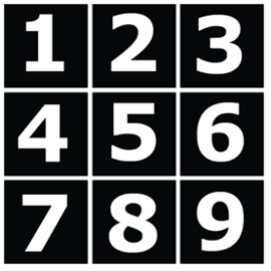
\includegraphics[width=0.3\linewidth]{Section3/2}
	\caption[Stitched square grid]{Example of sequence of frames in the stitched image if nine of them are included.}
	\vspace{-1.5em}
	\label{fig:stitched square grid}
\end{figure}
Another challenge we faced was to decide which frames should be included in the stitched image. To increase the algorithm’s robustness and to control better for interesting configurations that have some seemingly uninteresting frames interspersed throughout their evolutions, we created two additional parameters: the starting frame and the number of frames to be included. We tested many possible numerical values of the two parameters to discover the best combination. Figure ~\ref{fig:stitched image examples} shows two examples of the stitched images, one represents a boring rule while the other represents an interesting rule. 

\begin{figure}[H]
	\begin{subfigure}{0.45\textwidth}
     		\centering
     		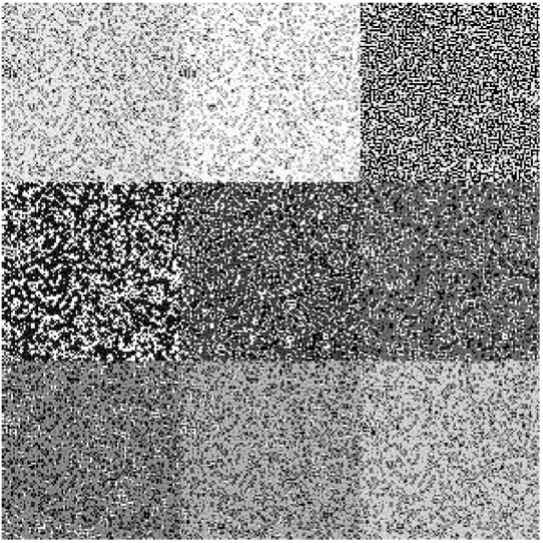
\includegraphics[width=\linewidth]{Section3/3.1}
   	\end{subfigure}
     	\begin{subfigure}{0.53\textwidth}
     		\centering
     		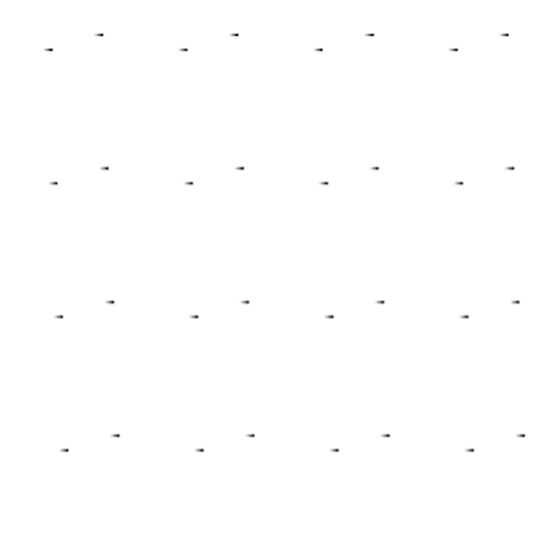
\includegraphics[width=\linewidth]{Section3/3.2}
   	\end{subfigure}
   	\caption[Examples of stitched images]{Examples of stitched up images. (Left) Nine frames are stitched together, which are generated by a boring rule “6/0,5,6,9”. All frames are noise. (Right) Sixteen frames are stitched together, which are generated interesting rule “2/2/8”. By comparing the frames in the top left and the bottom right corner, we could see the pattern translating to the right, which indicates a glider.}
   	\vspace{-1.5em}
   	\label{fig:stitched image examples}
\end{figure}

Since stitching frames is an uncanonical method of classifying cellular automata patterns, we wanted to measure the learnability of the stitched images using Brainome.ai \cite{Brainome} before we built the model. Because Brainome.ai accepts labeled data in CSV format, we needed to do feature extraction to the stitched images as the final pre-processing step. We first used a pre-trained NASNet-Large Model, which is a CNN that is trained on more than a million images from the ImageNet database \cite{ImageNet}. For each of the stitched images, the model returned 1000 selected features. We then fed the data into Brainome.ai and obtained corresponding information about Decision Trees and Neural Networks. The expected generalization using Decision Tree is 2.05 bits/bit and using a Neural Network is 0.19 bits/bit.  The decision tree has 1,026 parameters, and the estimated memory equivalent capacity for neural networks is 11,034 parameters. This overwhelming memory equivalent capacity indicated that the neural network would be extremely overfitting, which means that the features extracted were barely learnable by the neural network. This poor result was reasonable in retrospect because the NASNet-Large model is specifically used for classifying and extracting features from images of common-life objects, and cellular automata patterns is not one of the targeted objects. 

As our previous feature extraction method with NASNet-Large model was unsuccessful, we decided to directly use the pixels of the stitched images as features. We fed the data into Brainome.ai and learned that the estimated memory equivalent capacity for neural networks is 3217 parameters, which was much better than the previous result even though the risk of overfitting persisted. Nevertheless, this gave us sufficient confidence to proceed with model training. 

As raw data, these images were quite large given the RAM allocation of 12 Gigabytes by Google Colab \cite{Google Colab}. Running the notebook tended to crash the kernel so we settled for lower resolution and down sampled the pixel images to 300×300. This tradeoff allowed us to manipulate and do machine learning on the data without too much computational expense. As a final preprocessing step, the [0, 255] valued matrices representing the images were normalized using simple division to [0, 1]. This improved performance greatly in practice. Many of the model architectures we tried produced sub-baseline results before this step. The next part of the optimization process was a question of model architecture and hyperparameter tuning. We tried many things to create the best model, which includes altering the convolutional filter size, dense layers at output, pooling kernel size, type of pooling, dropout, and batch normalization. 

We found that the greatest improvements happened after adding dropout and batch normalization. There was also a significant increase in accuracy after increasing the convolutional filter size of the first convolutional layer to 5×5 from 3×3. We believed this is because 3×3 is too small to capture much of the complexity of the interesting configurations. Given a 3×3 window, many of the interesting shapes looked like noise.

We tried many things that did not work in addition to those that did. Increasing the pooling kernel size, using average pooling instead of max pooling, increasing the number of filters in the convolutional layers (from 64 in each), and increasing the second convolutional layer’s filter size from 3×3 to 5×5, all resulted in worse performance by the validation accuracy metric. We found that increasing the epochs past 30 resulted in overfitting. Eventually, we used the architecture described in Table ~\ref{table:CNN structure}. The amount of time it took to train the model depended on greatly the number of training epochs and the size of the dataset, but it would not exceed an hour in our case. 

The machine learner was able to achieve 93.44\% training accuracy and 84.12\% testing accuracy on the testing set with 10\% interesting data. The test recall is 100\%, indicating every interesting configuration has been correctly labeled as such. 

\begin{table}[H]
	\begin{center}
		\begin{tabular}{ | m{2cm} | m{8cm} | } 
			\hline
			Conv2D & 64 filter output space, 5×5 filters, ReLU activation. Batch normalization prior to ReLU \\ 
			\hline
			max pooling & (2, 2) pooling kernels, 15\% dropout  \\ 
			\hline
			Conv2D & 64 filter output space, 3×3 filters, ReLU activation. Batch normalization prior to ReLU  \\ 
			\hline
			max pooling & (2, 2) pooling kernels, 15\% dropout \\ 
			\hline
			dense layer & 64 nodes, ReLU activation, 15\% dropout  \\ 
			\hline
			dense layer & 10 nodes, ReLU activation, 15\% dropout  \\ 
			\hline
			output layer & 1 node, sigmoid activation \\
			\hline
		\end{tabular}
	\caption{Structure of the CNN}
	\label{table:CNN structure}
	\vspace{-1.5em}
	\end{center}
\end{table}

\subsection{Entropy Analysis}
Due to the varying degrees of information density in cellular automata patterns, entropy is an adequate measure to use since there is likely a correlation between the label (boring and interesting) and the degree of randomness in the images created by the cellular automata. There are many existing research on this topic and the common consensus is that the problem of computing or even approximating the topological entropy of a given cellular automata is algorithmically undecidable \cite{entropy, entropy-two}. Therefore, we decided to try something that has not yet been attempted before. Namely, we decided to compute the cross-entropy values of the stitched images generated in the preprocessing step of Section ~\ref{CNN Training}. In this case, boredom can be understood as either static or complete noise, which correspond to extremely low and high entropy values. 

We used cross-entropy as the default entropy function. We iterated through all the stitched frames and computed their entropies using the cross-entropy algorithm, then plotted the entropy values of the boring and interesting images in Figure ~\ref{fig:entropy distribution}. 
\begin{figure}[H]
	\begin{subfigure}{0.5 \textwidth}
		\centering
		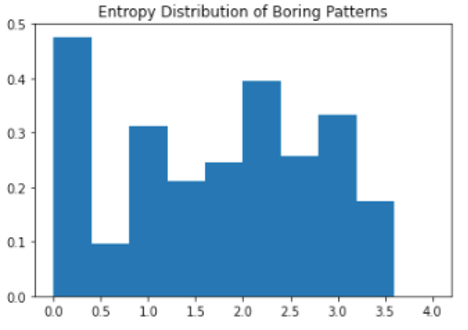
\includegraphics[width=\linewidth]{Section3/4.1}
	\end{subfigure}
	\begin{subfigure}{0.5 \textwidth}
		\centering
		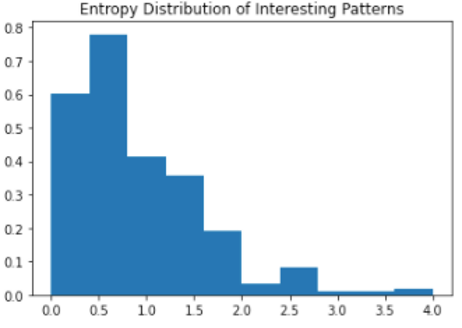
\includegraphics[width=\linewidth]{Section3/4.2}
	\end{subfigure}
	\caption[Entropy distribution of patterns]{Entropy distribution of boring (left) and interesting (right) patterns.}
	\label{fig:entropy distribution}
	\vspace{-1.5em}
\end{figure}

Boring images had entropy values that spread roughly evenly from 0.0 to 3.5, with a small gap between 0.5 and 0.75. Many had entropy values close to 0.0, which is reasonable because they would likely correspond to patterns that die out. On the other hand, interesting images had entropy values concentrated in the 0.0 to 2.0 range, especially between 0.5 and 0.75. This intuitively makes sense because interesting images had less noise and entropy compared to boring images on average. It should be noted the minimum entropy for boring images was 0.0 while the minimum entropy for interesting images was 0.0318. This is because frames that had no live cells were always labeled as boring. The entropy values suggest adding features identifying if the image entropy is above 2.0 or equals to exactly 0 may be beneficial for the model accuracy. 

\newpage
\section{Glider Discoveries}
\label{Glider Discoveries}
After we finished training the machine learners, we put them into practice and used them to classify patterns and find gliders in those that are interesting. Since cellular automata with two possible states, like the Game of Life, have already been widely explored, we focused mainly on those with three states. We ran the machine learner on the sequences of frames generated from random combinations of survival and born rules, and then manually inspected the few rules which the learner classified as interesting. Overall this was a very time-consuming process since for each new rule, we had to generate a sequence of frames so that the machine learner can have something to train on. However, we believed that the situation could be ameliorated in the future thanks to the process being entirely parallelizable. More relavant information is discussed in Section ~\ref{Future Work}. The evolution of the gliders in this section will be provided as a sequence of figures. The numbers give the generations and the exact movement of each is depicted by its shifting position in the enclosing grids. Code used to generate the figures can be found in ~\ref{subsection:Glider Image and GIF generation} and ~\ref{subsection:Initial configuration of the gliders}. 

\subsection{Gliders in three-state cellular automata}
Our machine learner has found several new interesting rules with three states (the dead state, the live state, and one sick state) that have not been previously discovered, which are “4,6/2/3”, “4/2,4/3”, “4,6/2,4/3”, “4,6/2,4/3”, “4/2,5/3”, “3,6/2,6/3”, “5,6/2,6/3”. The common trait of these newly discovered rules is that dead cells will be born with two alive cells in their neighborhoods. These rules all generate the same family of gliders, where the members are all led by a two-by-two glider and followed with a distinct \textit{tagalong}, where tagalong is defined as a pattern that is not a glider itself but can be attached to the back of a glider to form a larger glider \cite{spaceship}. We decided to call this two-by-two leading structure the “leading block” (top left corner in Figure ~\ref{fig:one-period gliders}). The leading block is the smallest found glider in all patterns with three possible states. It has a period of one and a speed of $c$. Since all members in the family are led by the leading block, they all have a uniform speed of $c$. However, the members can have different periods. The one-period members have zero or more one-by-two blocks (we named it the supplemental block), which are the smallest possible tagalongs, attached to either side of the leading block. We can enumerate the number of one-period gliders with at most two supplemental blocks. There is one member with no supplemental block attached, namely the leading block, four members with one, and eighteen members with two. These gliders are shown in Figure ~\ref{fig:one-period gliders}. There are infinitely many one-period members in the family because any arbitrary number of supplemental blocks can be attached. 

However, one caveat is that there are some patterns, like the one shown in ~\ref{fig:counter example}, that have the supplemental blocks attached to the leading block but are not actually gliders. This means that the tagalongs are very delicate and the slightest difference in their structure can lead to a massive change in the eventual outcome. Most patterns that have almost the same tagalong as one of the basic forms with only a few different cells will not turn out to be a glider. Thus, it is very hard to artificially engineer a glider and proves Wolfram's philosophy that we should not try to build anything at all. 

\begin{figure}[H]
	\begin{center}
		{\Huge$\uparrow$}
	\end{center}
 	\begin{subfigure}{0.49\textwidth}
     		\centering
     		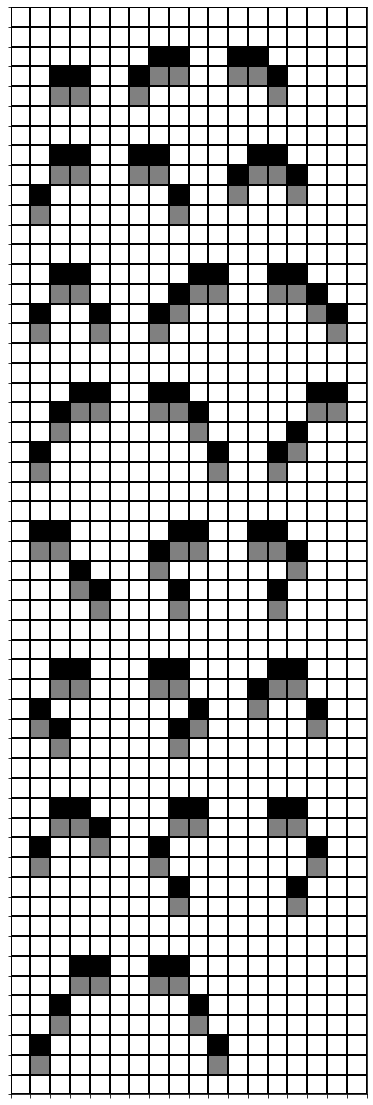
\includegraphics[width=\linewidth]{Section4/1.0}
   	\end{subfigure}
     	\begin{subfigure}{0.49\textwidth}
     		\centering
     		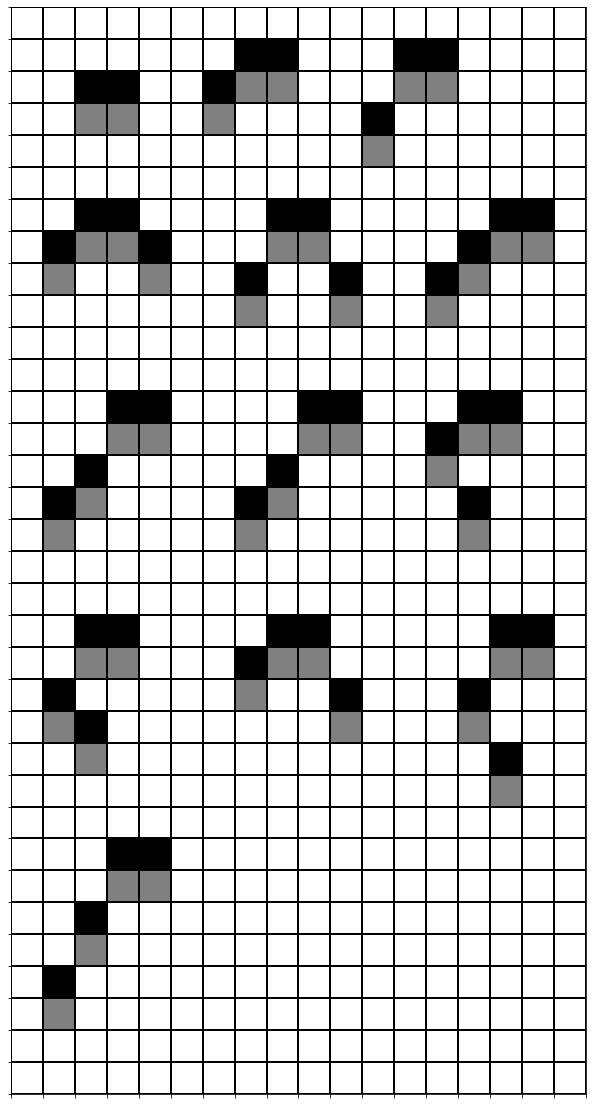
\includegraphics[width=\linewidth]{Section4/1.1}
   	\end{subfigure}
   	\caption[One-period gliders]{All one-period members with zero, one, or two supplemental blocks of the glider family that appears in rules “4,6/2/3”, “2,4,6/2,4/3”, “4,6/2,4/3”, “3,6/2,6/3”, “5,6/2,6/3”. Code is provided in ~\ref{subsubsection:one-period gliders}.}
   	\label{fig:one-period gliders}
   	\vspace{-1.5em}
\end{figure}

\begin{figure}[H]
	\begin{center}
		{\Huge$\uparrow$}
	\end{center}
	\begin{subfigure}{0.19\textwidth}
     		\centering
     		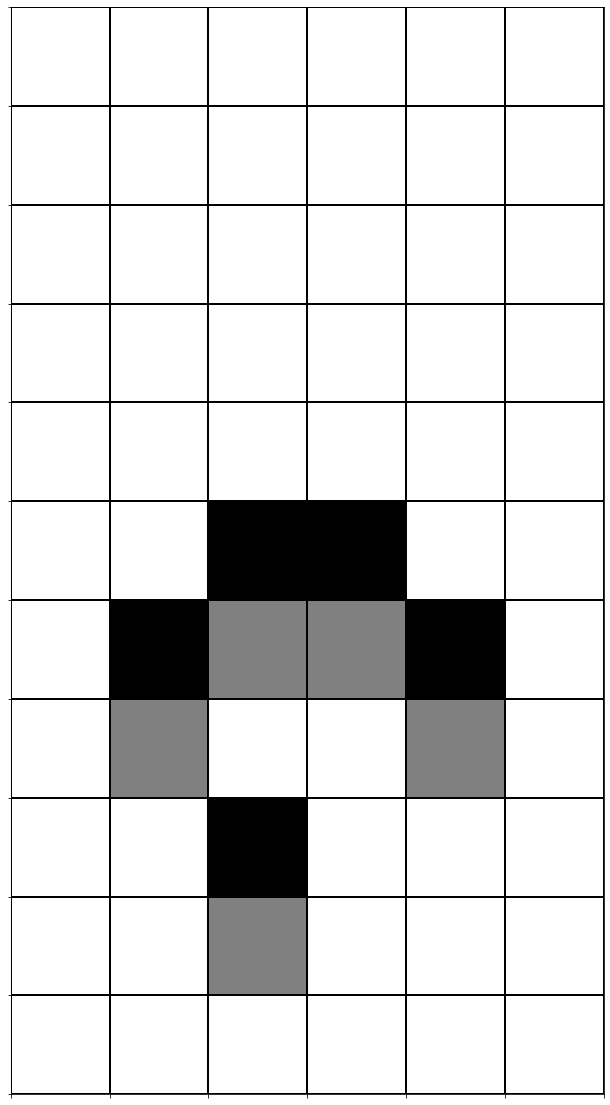
\includegraphics[width=\linewidth]{Section4/2.0}
   	\end{subfigure}
     	\begin{subfigure}{0.19\textwidth}
     		\centering
     		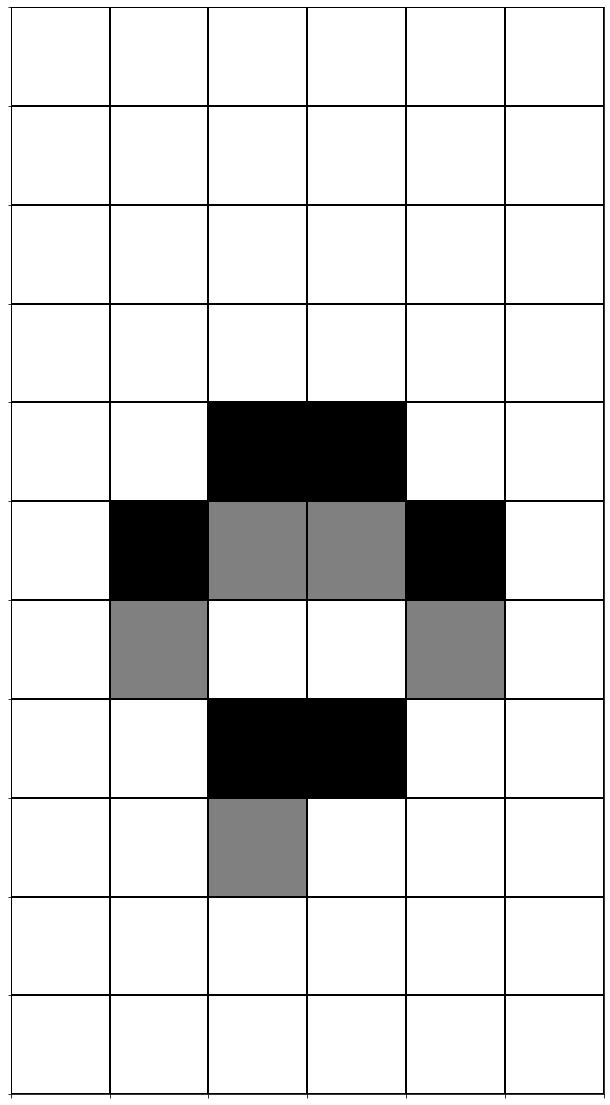
\includegraphics[width=\linewidth]{Section4/2.1}
   	\end{subfigure}
        \begin{subfigure}{0.19\textwidth}
     		\centering
     		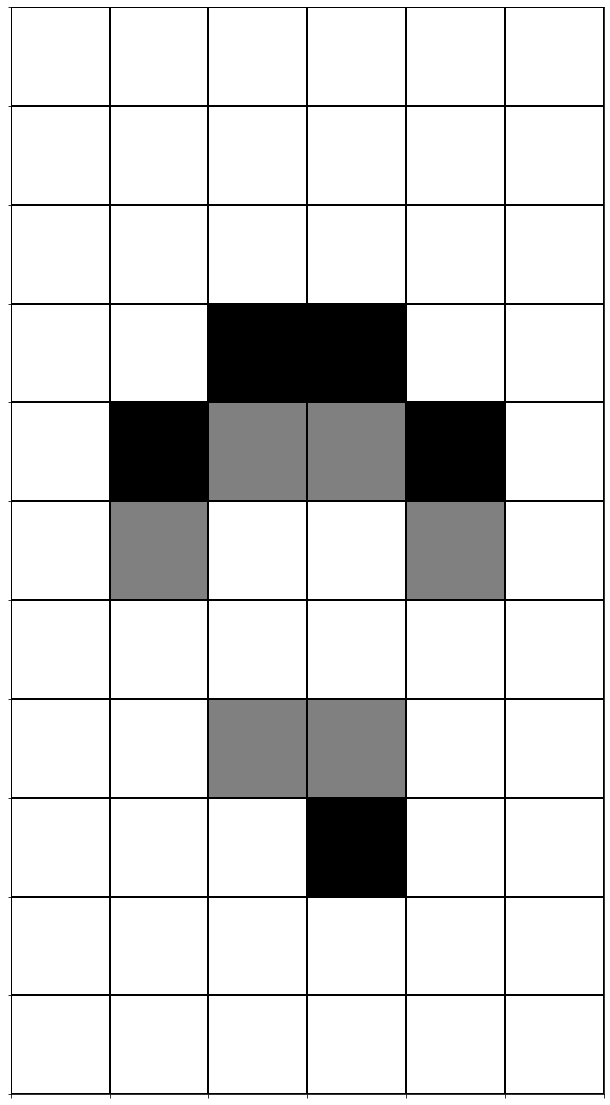
\includegraphics[width=\linewidth]{Section4/2.2}
   	\end{subfigure}
        \begin{subfigure}{0.19\textwidth}
     		\centering
     		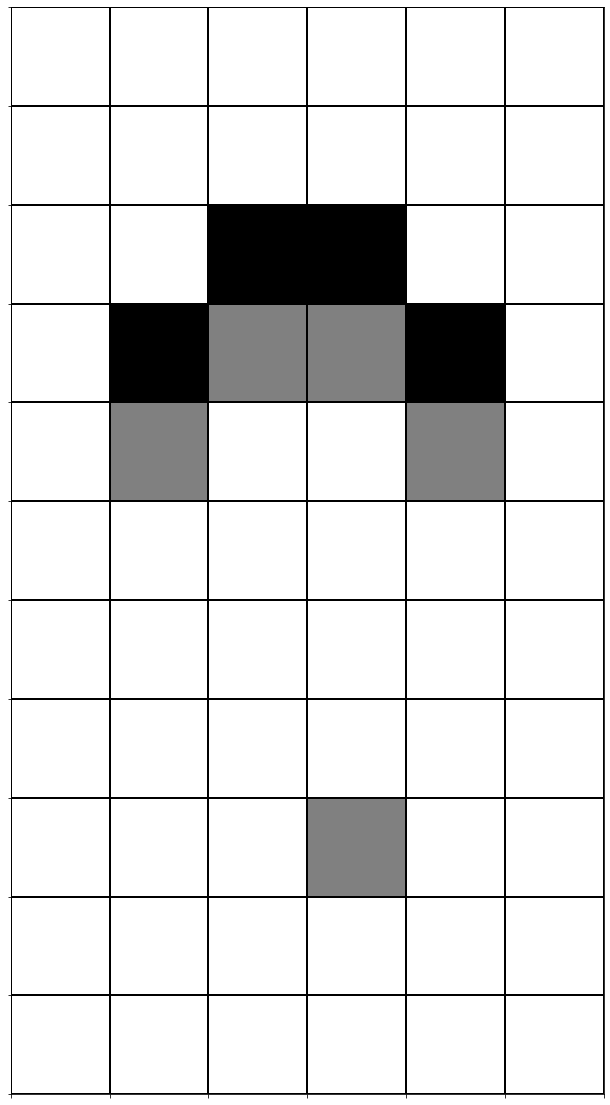
\includegraphics[width=\linewidth]{Section4/2.3}
   	\end{subfigure}
        \begin{subfigure}{0.19\textwidth}
     		\centering
     		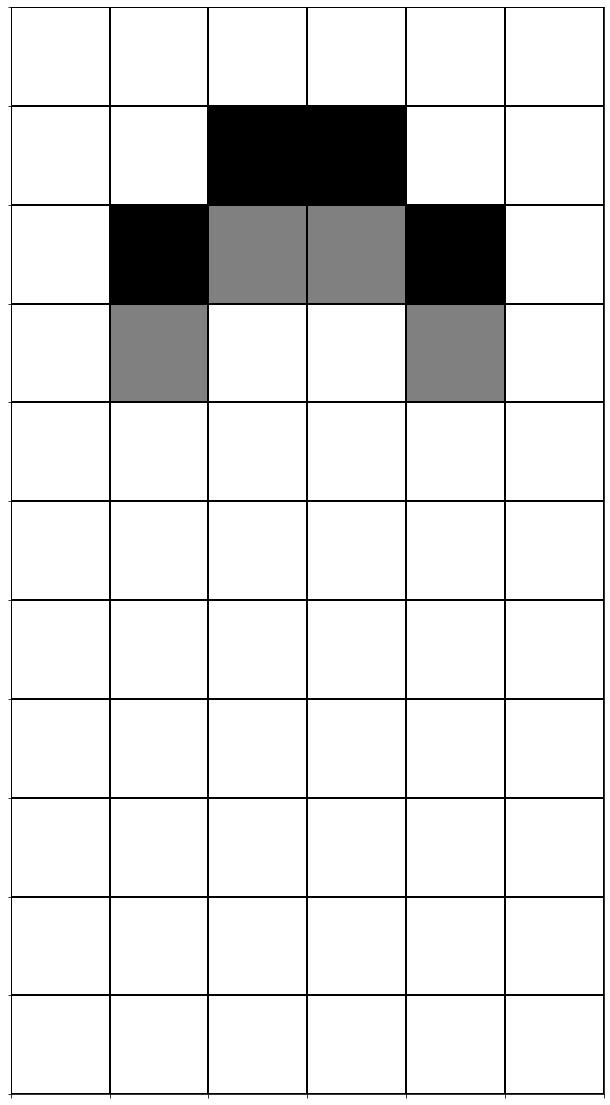
\includegraphics[width=\linewidth]{Section4/2.4}
   	\end{subfigure}
   	\caption[A non-glider that looks like one]{A pattern that is not a glider in rules “4,6/2/3”, “(2)4,6/2,4/3”, “4,6/2,4/3”, “3,6/2,6/3”, “5,6/2,6/3” despite consisting of the leading block and three supplemental blocks. However, it does transform into another two-period glider in four steps. Code is provided in ~\ref{subsubsection:counter example}.}
   	\label{fig:counter example}
   	\vspace{-1.5em}
\end{figure}

We also found many family members with a period of two. Their structures are more complicated since their tagalongs are no longer entirely made of the supplemental blocks. They emit one unit of vanishing "exhaust" when moving across the grid, whereas the rest of their body remains unchanged. We have discovered five most basic two-period gliders that appear in rules “4,6/2/3”, “4,6/2,4/3”, “4,6/2,4/3”, “3,6/2,6/3”, and “5,6/2,6/3” in Figure ~\ref{fig:two-period gliders}, each with a distinct tagalong. For simplicity, they will be referred to as “two-period glider A, B, C, D, and E” in the rest of the report. Furthermore, we have also observed some two-period gliders that have the exact same tagalongs as the five basic forms. For example, in Figure ~\ref{fig:almost same two-period glider} is another glider that looks virtually the same as the “two-period glider E” and only differs in the way that its tagalong is relatively moved towards the right by one unit. We have already seen such room for diversity in the one-period members. Additionally, like the one-period members, there are also infinitely many two-period gliders in the family. Their tagalongs can get arbitrarily large as they can have a connecting bridge consisting of any arbitrary number of supplemental between the basic tagalong and the two-by-two leading block. However, all of these tagalongs are essentially extensions of one of the five most basic forms in Figure ~\ref{fig:tagalongs of two-period gliders}. This means that their tagalongs can be reduced by stripping away one or more supplemental blocks. Figure ~\ref{fig:extended two-period gliders} depicts some possible extensions of the basic five two-period gliders. 

\begin{figure}[H]
	\begin{subfigure}[t]{0.03\textwidth}
    		\textbf{A}
  	\end{subfigure}
 	\begin{subfigure}{0.3\textwidth}
     		\centering
     		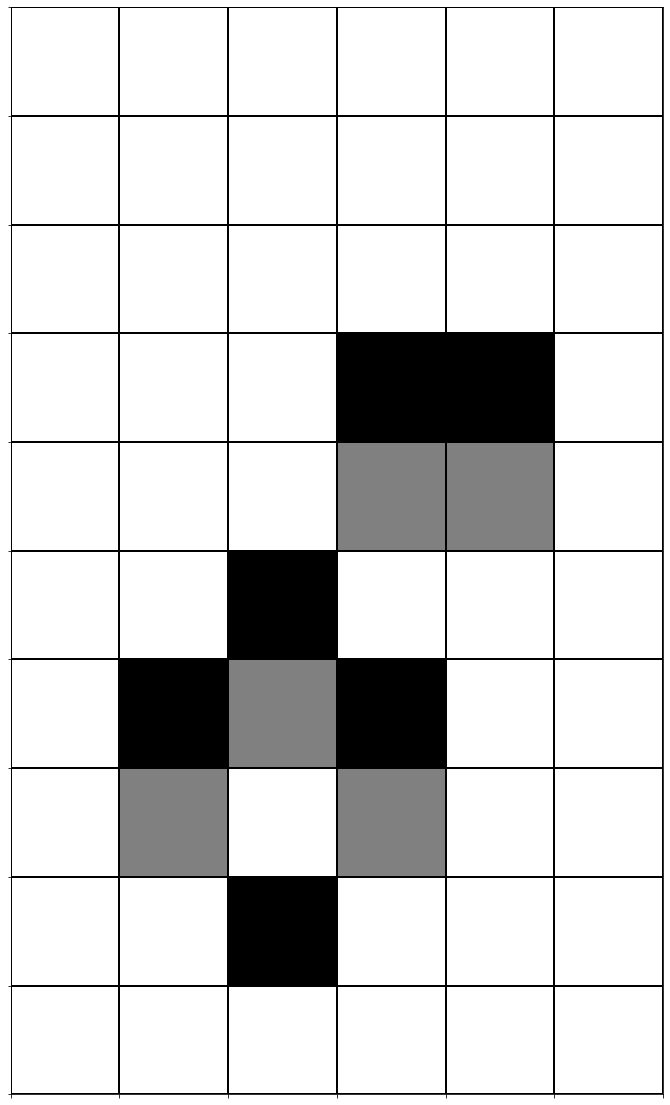
\includegraphics[angle=270,width=\linewidth]{Section4/3.0}
     		\subcaption{}
   	\end{subfigure}
     	\begin{subfigure}{0.3\textwidth}
     		\centering
     		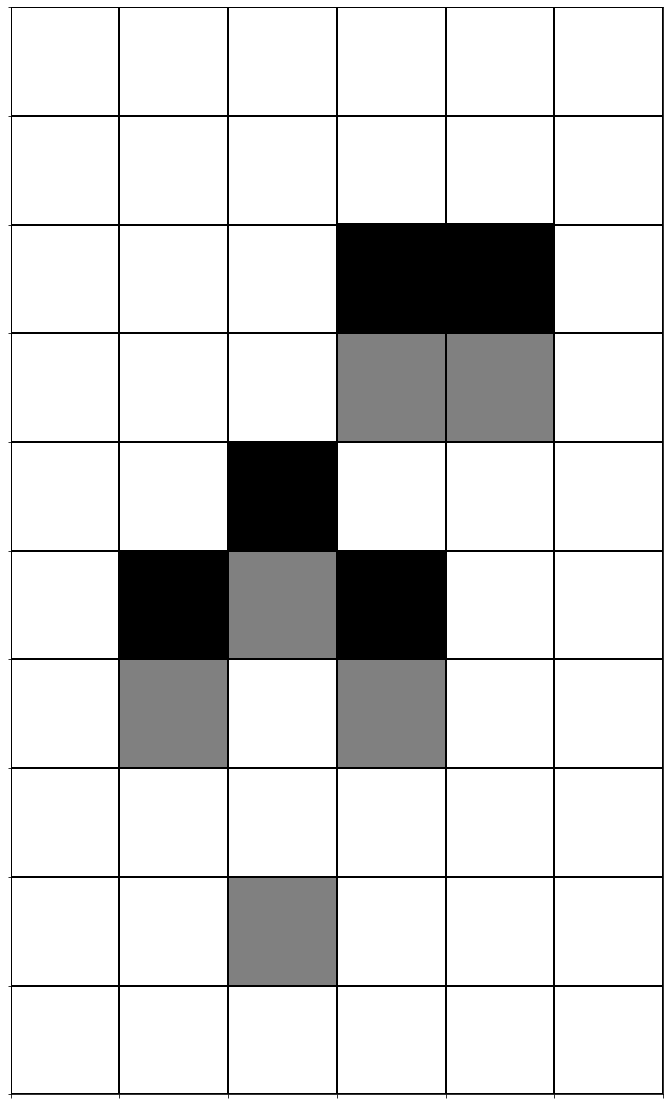
\includegraphics[angle=270,width=\linewidth]{Section4/3.1}
     		\subcaption{}
   	\end{subfigure}
        	\begin{subfigure}{0.3\textwidth}
     		\centering
     		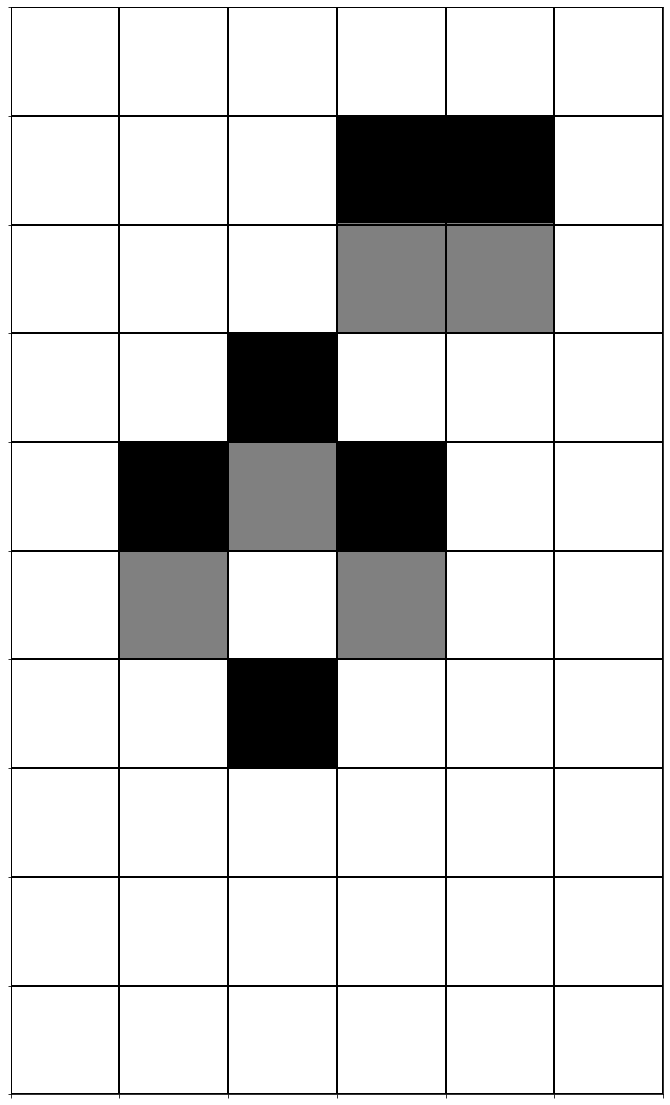
\includegraphics[angle=270,width=\linewidth]{Section4/3.2}
     		\subcaption{}
   	\end{subfigure}
   	\begin{subfigure}[t]{0.03\textwidth}
      		{\LARGE$\xrightarrow{}$}
   	\end{subfigure}
      	\newline
   	\setcounter{subfigure}{0}
     	\begin{subfigure}[t]{0.03\textwidth}
    		\textbf{B}
  	\end{subfigure}
   	\begin{subfigure}{0.3\textwidth}
    		\centering
     		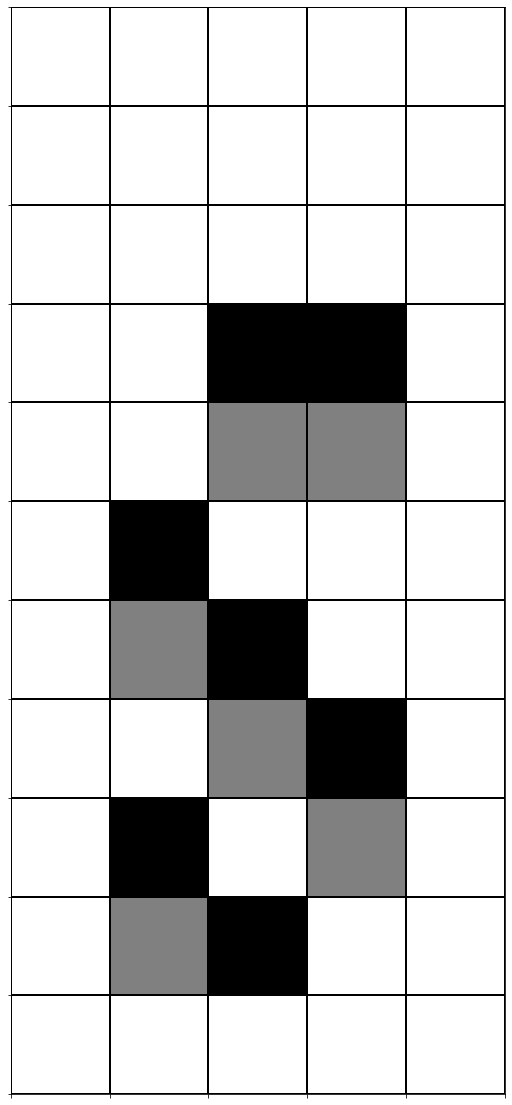
\includegraphics[angle=270,width=\linewidth]{Section4/4.0}
     		\subcaption{}
   	\end{subfigure}
     	\begin{subfigure}{0.3\textwidth}
     		\centering
     		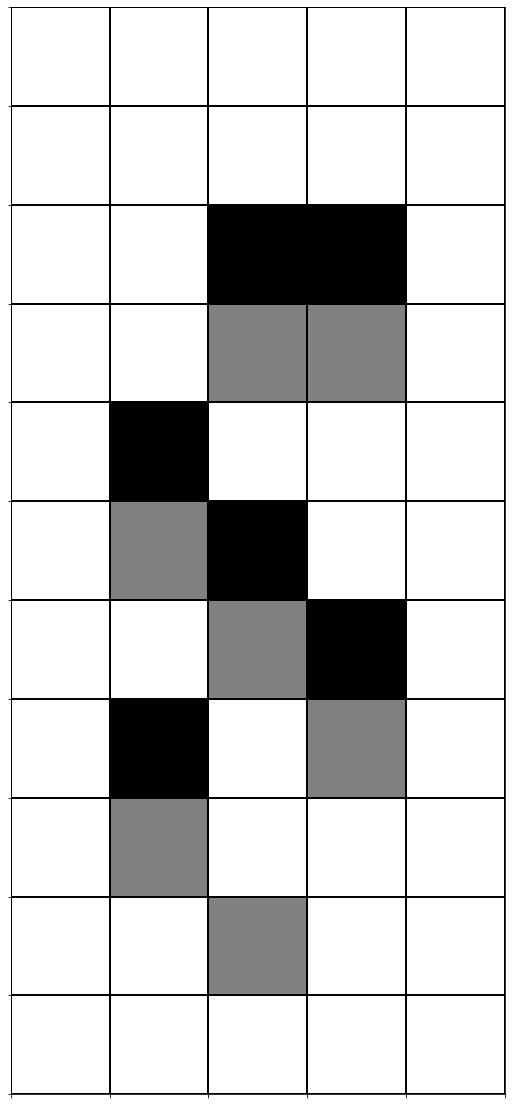
\includegraphics[angle=270,width=\linewidth]{Section4/4.1}
     		\subcaption{}
   	\end{subfigure}
        \begin{subfigure}{0.3\textwidth}
     		\centering
     		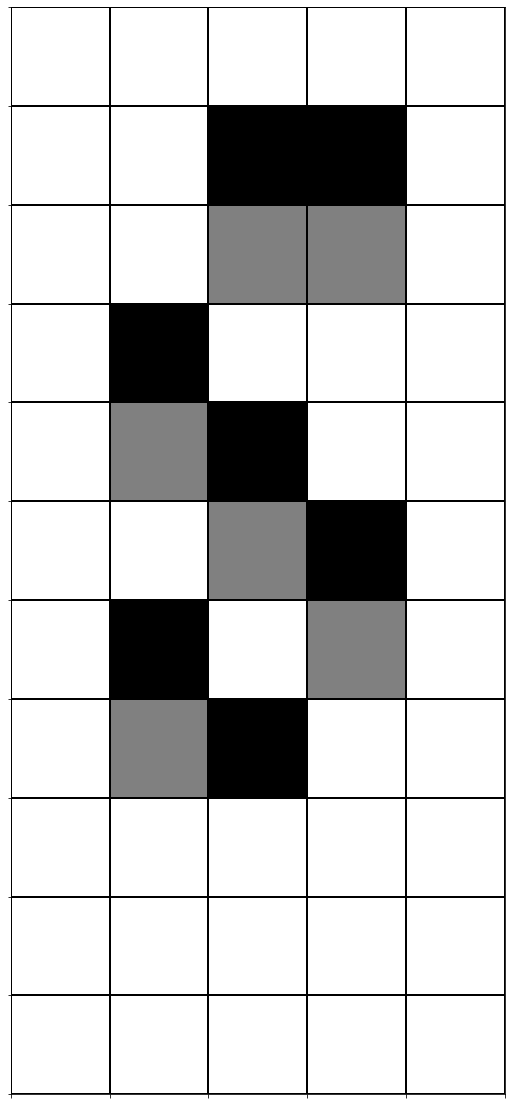
\includegraphics[angle=270,width=\linewidth]{Section4/4.2}
     		\subcaption{}
   	\end{subfigure}
	\begin{subfigure}[t]{0.03\textwidth}
      		{\LARGE$\xrightarrow{}$}
	\end{subfigure}
      	\newline
   	\setcounter{subfigure}{0}
     	\begin{subfigure}[t]{0.03\textwidth}
    		\textbf{C}
  	\end{subfigure}	
      	\begin{subfigure}{0.3\textwidth}
    		\centering
     		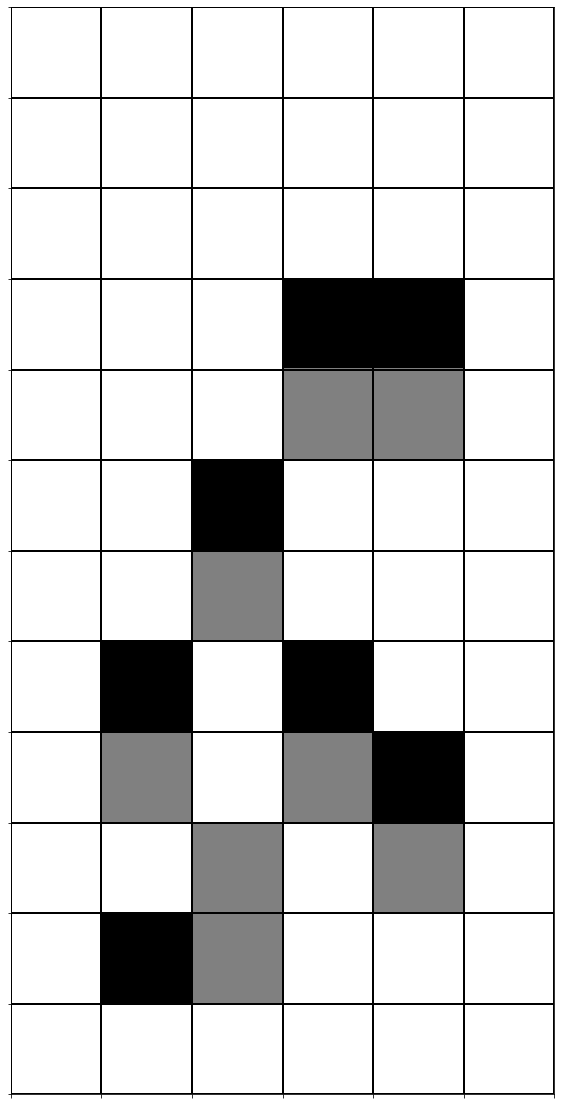
\includegraphics[angle=270,width=\linewidth]{Section4/5.0}
     		\subcaption{}
   	\end{subfigure}
     	\begin{subfigure}{0.3\textwidth}
     		\centering
     		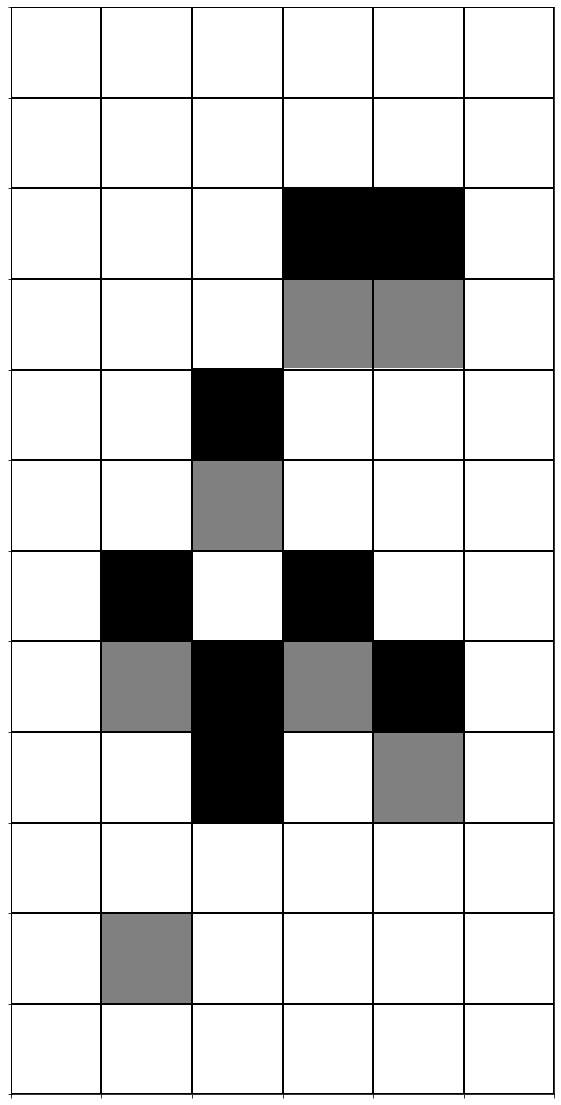
\includegraphics[angle=270,width=\linewidth]{Section4/5.1}
     		\subcaption{}
   	\end{subfigure}
        \begin{subfigure}{0.3\textwidth}
     		\centering
     		\includegraphics[angle=270,width=\linewidth]{Section4/5.2}
     		\subcaption{}
   	\end{subfigure}
	\begin{subfigure}[t]{0.03\textwidth}
      		{\LARGE$\xrightarrow{}$}
	\end{subfigure}
      	\newline
   	\setcounter{subfigure}{0}
     	\begin{subfigure}[t]{0.03\textwidth}
    		\textbf{D}
  	\end{subfigure}		
         \begin{subfigure}{0.3\textwidth}
     		\centering
     		\includegraphics[angle=270,width=\linewidth]{Section4/6.0}
     		\subcaption{}
   	\end{subfigure}
     	\begin{subfigure}{0.3\textwidth}
     		\centering
     		\includegraphics[angle=270,width=\linewidth]{Section4/6.1}
     		\subcaption{}
   	\end{subfigure}
        \begin{subfigure}{0.3\textwidth}
     		\centering
     		\includegraphics[angle=270,width=\linewidth]{Section4/6.2}
     		\subcaption{}
   	\end{subfigure}
	\begin{subfigure}[t]{0.03\textwidth}
      		{\LARGE$\xrightarrow{}$}
	\end{subfigure}
      	\newline
   	\setcounter{subfigure}{0}
     	\begin{subfigure}[t]{0.03\textwidth}
    		\textbf{E}
  	\end{subfigure}		
        \begin{subfigure}{0.3\textwidth}
     		\centering
     		\includegraphics[angle=270,width=\linewidth]{Section4/7.0}
     		\subcaption{}
   	\end{subfigure}
     	\begin{subfigure}{0.3\textwidth}
     		\centering
     		\includegraphics[angle=270,width=\linewidth]{Section4/7.1}
     		\subcaption{}
   	\end{subfigure}
        \begin{subfigure}{0.3\textwidth}
     		\centering
     		\includegraphics[angle=270,width=\linewidth]{Section4/7.2}
     		\subcaption{}
   	\end{subfigure}
	\begin{subfigure}[t]{0.03\textwidth}
      		{\LARGE$\xrightarrow{}$}
	\end{subfigure}
   
	\caption[Two-period gliders]{The five basic two-period members of the glider family that exist for rules “4,6/2/3”, “4,6/2,4/3”, “4,6/2,4/3”, “3,6/2,6/3”, “5,6/2,6/3”. For simplicity, they are referred to as “two-period glider A, B, C, D, and E” respectively. Code is provided in ~\ref{subsubsection:two-period gliders(1/5)}, ~\ref{subsubsection:two-period gliders(2/5)}, ~\ref{subsubsection:two-period gliders(3/5)}, ~\ref{subsubsection:two-period gliders(4/5)}, and ~\ref{subsubsection:two-period gliders(5/5)}.}
   	\label{fig:two-period gliders}
   	\vspace{-1.5em}
\end{figure}

\begin{figure}[H]
	\begin{subfigure}{0.18\textwidth}
     		\centering
     		\includegraphics[angle=270,width=\linewidth]{Section4/8.0}
    		\subcaption{}
   	\end{subfigure}
     	\begin{subfigure}{0.18\textwidth}
     		\centering
     		\includegraphics[angle=270,width=\linewidth]{Section4/8.1}
     		\subcaption{}
   	\end{subfigure}
        \begin{subfigure}{0.18\textwidth}
     		\centering
     		\includegraphics[angle=270,width=\linewidth]{Section4/8.2}
     		\subcaption{}
   	\end{subfigure}
        	\begin{subfigure}{0.18\textwidth}
     		\centering
     		\includegraphics[angle=270,width=\linewidth]{Section4/8.3}
     		\subcaption{}
   	\end{subfigure}
        \begin{subfigure}{0.18\textwidth}
     		\centering
     		\includegraphics[angle=270,width=\linewidth]{Section4/8.4}
     		\subcaption{}
   	\end{subfigure}
      	\newline
   	\caption[Tagalongs of the two-period gliders]{The five basic tagalongs of two-period gliders.}
   	\label{fig:tagalongs of two-period gliders}
\end{figure}

\begin{figure}[H]
	\begin{subfigure}{0.3\textwidth}
     		\centering
     		\includegraphics[angle=270,width=\linewidth]{Section4/9.0}
     		\subcaption{}
   	\end{subfigure}
     	\begin{subfigure}{0.3\textwidth}
     		\centering
     		\includegraphics[angle=270,width=\linewidth]{Section4/9.1}
     		\subcaption{}
   	\end{subfigure}
        \begin{subfigure}{0.3\textwidth}
     		\centering
     		\includegraphics[angle=270,width=\linewidth]{Section4/9.2}
     		\subcaption{}
   	\end{subfigure}
   {\LARGE$\xrightarrow{}$}
   \setcounter{subfigure}{0}
   \caption[Similar two-period glider]{The glider that is almost the same as “two-period glider E” except its tagalong is moved relatively towards right by one unit. Code is provided in ~\ref{subsubsection:almost same two-period glider}.}
   \label{fig:almost same two-period glider}
   \vspace{-1.5em}
\end{figure}

\begin{figure}[H]
	\begin{subfigure}{0.3\textwidth}
     		\centering
     		\includegraphics[angle=270,width=\linewidth]{Section4/10.0}
     		\subcaption{}
   	\end{subfigure}
     	\begin{subfigure}{0.3\textwidth}
     		\centering
     		\includegraphics[angle=270,width=\linewidth]{Section4/10.1}
     		\subcaption{}
   	\end{subfigure}
        \begin{subfigure}{0.3\textwidth}
     		\centering
     		\includegraphics[angle=270,width=\linewidth]{Section4/10.2}
     		\subcaption{}
   	\end{subfigure}
      	{\LARGE$\xrightarrow{}$}
      	\newline
   	\setcounter{subfigure}{0}
   	\begin{subfigure}{0.3\textwidth}
     		\centering
     		\includegraphics[angle=270,width=\linewidth]{Section4/11.0}
     		\subcaption{}
   	\end{subfigure}
     	\begin{subfigure}{0.3\textwidth}
     		\centering
     		\includegraphics[angle=270,width=\linewidth]{Section4/11.1}
     		\subcaption{}
   	\end{subfigure}
        \begin{subfigure}{0.3\textwidth}
     		\centering
     		\includegraphics[angle=270,width=\linewidth]{Section4/11.2}
     		\subcaption{}
   	\end{subfigure}
     	{\LARGE$\xrightarrow{}$}
      	\newline
   	\setcounter{subfigure}{0}
      	\begin{subfigure}{0.3\textwidth}
     		\centering
     		\includegraphics[angle=270,width=\linewidth]{Section4/12.0}
     		\subcaption{}
   	\end{subfigure}
     	\begin{subfigure}{0.3\textwidth}
     		\centering
     		\includegraphics[angle=270,width=\linewidth]{Section4/12.1}
     		\subcaption{}
   	\end{subfigure}
        \begin{subfigure}{0.3\textwidth}
     		\centering
     		\includegraphics[angle=270,width=\linewidth]{Section4/12.2}
     		\subcaption{}
   	\end{subfigure}
      	{\LARGE$\xrightarrow{}$}
      	\newline
   	\setcounter{subfigure}{0}
         \begin{subfigure}{0.3\textwidth}
     		\centering
     		\includegraphics[angle=270,width=\linewidth]{Section4/13.0}
     		\subcaption{}
   	\end{subfigure}
     	\begin{subfigure}{0.3\textwidth}
     		\centering
     		\includegraphics[angle=270,width=\linewidth]{Section4/13.1}
     		\subcaption{}
  	\end{subfigure}
        \begin{subfigure}{0.3\textwidth}
     		\centering
     		\includegraphics[angle=270,width=\linewidth]{Section4/13.2}
     		\subcaption{}
   	\end{subfigure}
      	{\LARGE$\xrightarrow{}$}
      	\newline
   	\setcounter{subfigure}{0}
     	\begin{subfigure}{0.3\textwidth}
     		\centering
     		\includegraphics[angle=270,width=\linewidth]{Section4/14.0}
     		\subcaption{}
   	\end{subfigure}
     	\begin{subfigure}{0.3\textwidth}
     		\centering
     		\includegraphics[angle=270,width=\linewidth]{Section4/14.1}
     		\subcaption{}
   	\end{subfigure}
        \begin{subfigure}{0.3\textwidth}
     		\centering
     		\includegraphics[angle=270,width=\linewidth]{Section4/14.2}
     		\subcaption{}
   	\end{subfigure}
      	{\LARGE$\xrightarrow{}$}
   	\setcounter{subfigure}{0}
   	\caption[Extended two-period gliders]{Examples of extended two-period members of the glider family that exist for rules “4,6/2/3”, “4,6/2,4/3”, “4,6/2,4/3”, “3,6/2,6/3”, “5,6/2,6/3”. Their tagalongs are the same as the five basic forms in Figure 4.4 except there is an additional supplemental block connecting them to the leading block. The leading block is like the tractor towing something behind it and this one simply has a longer tow cable. Other extended members have more connecting supplemental blocks and thus even longer tow cables. Code is provided in ~\ref{subsubsection:extended two-period gliders(1/5)}, ~\ref{subsubsection:extended two-period gliders(2/5)}, ~\ref{subsubsection:extended two-period gliders(3/5)}, ~\ref{subsubsection:extended two-period gliders(4/5)}, and ~\ref{subsubsection:extended two-period gliders(5/5)}. }
   	\label{fig:extended two-period gliders}
   	\vspace{-1.5em}
\end{figure}

We have also found family members with a period of four. Superficially, they do not look much different from the two-period members except their tagalongs are larger and more complicated. They emit a more noticeable and larger amount of vanishing exhaust when they move across the grid. We identified six basic four-period members shown in Figure ~\ref{fig:four-period gliders}, each with a distinct tagalong in Figure ~\ref{fig:tagalongs of four-period gliders}. For simplicity, they will be referred to as “four-period glider A, B, C, D, E and F” in the rest of the report. The longest period members we found are the ones with periods of eight in Figure ~\ref{fig:eight-period gliders}. We have discovered a total of two such gliders, which we will name as “eight-period glider A” and “eight-period glider B”. Their tagalongs are depicted in Figure ~\ref{fig:tagalongs of eight-period gliders}. Superficially, there is an uncanny resemblance between “eight-period glider A” and “four-period glider C”, and “eight-period glider B” and “four-period glider A”. The two eight-period gliders both generate a maximum of ten units’ exhaust. We believe it is highly likely that there are more with unique tagalongs that are yet undiscovered, as they are more rare and thus much harder to find than the other members in the family. With the same argument we made with the two-period gliders, there are infinitely many four and eight-period gliders in the family. 

The family members introduced so far have only one tail. However, these gliders, unlike normal species in real life, have unlimited potential to mutate, combine, and have arbitrarily complex structures. However, some members in the family have found a way to combine some of the basic tagalongs to form a larger one. Figure ~\ref{fig:Frankenstein gliders} shows two Frankenstein gliders whose tagalong is a combination of the basic forms we have introduced earlier. One combines “two-period glider C” and “four-period glider A”. The other combines “two-period glider A” and two “four-period glider B”s. Their existence proves that two or more tagalongs can be combined to form a larger tagalong. The period of the resulting Frankenstein glider is determined by the longer period of its components. The diversity of the family members is thus beyond imaginable as the tagalongs can get arbitrarily complex and it is impossible to enumerate all possible tagalongs. 

The most interesting family members we found are rakes, which are cellular automata that leave behind a trail of non-vanishing debris of a stream of gliders \cite{rake}. Their structures are much more complex than the other family members. We have observed a total of three rakes, one with a period of four and two with eight in Figure ~\ref{fig:four-period rake}, Figure ~\ref{fig:eight-period rake one}, and Figure ~\ref{fig:eight-period rake two}. For simplicity, they will be referred to as “rake A, B, and C” in the rest of the report. Their periods are equivalent to the number of steps it takes them to generate a new glider. All three rakes generate a stream of one-period gliders, whose moving directions are not the same as the rakes. Rake A generates a stream of two-by-two leading blocks, which moves in the opposite direction as the rake itself. Rake B generates a stream of one-period members with one supplemental block, which also moves in the opposite direction as the rake itself. Rake C generates a stream of one-period members with two supplemental blocks, which move perpendicular to the rake. 

We discovered one special glider depicted in Figure ~\ref{fig:the new life} that does not contain the leading block and hence is not a member of the family. It maintains a total of three live and three sick cells in all generations. Furthermore, the gliders we have introduced so far either traverse horizontally or vertically. But just like Conway’s Game of Life glider, this glider moves diagonally across the grid with a period of four. Its speed is also $\frac{c}{4}$, since it takes four generations for a given state to be translated by one cell. We decided to call this the new Life with three states.
\begin{figure}[H]
	\begin{subfigure}{0.16\textwidth}
     		\centering
     		\includegraphics[width=\linewidth]{Section4/21.0}
     		\subcaption{}
   	\end{subfigure}
     	\begin{subfigure}{0.16\textwidth}
     		\centering
     		\includegraphics[width=\linewidth]{Section4/21.1}
     		\subcaption{}
   	\end{subfigure}
        \begin{subfigure}{0.16\textwidth}
     		\centering
     		\includegraphics[width=\linewidth]{Section4/21.2}
     		\subcaption{}
   	\end{subfigure}
        	\begin{subfigure}{0.16\textwidth}
     		\centering
     		\includegraphics[width=\linewidth]{Section4/21.3}
     		\subcaption{}
   	\end{subfigure}
        	\begin{subfigure}{0.16\textwidth}
     		\centering
     		\includegraphics[width=\linewidth]{Section4/21.4}
     		\subcaption{}
   	\end{subfigure}
	\begin{subfigure}{0.16\textwidth}
     		\centering
     		\includegraphics[width=\linewidth]{Section4/21.5}
     	\subcaption{}
   	\end{subfigure}
      	\newline
   	\setcounter{subfigure}{0}
	\caption[Tagalongs of four-period gliders]{The six basic tagalongs of the four-period gliders.}
	\label{fig:tagalongs of four-period gliders}
\end{figure}

\begin{figure}[H]
\begin{center}
{\Huge$\uparrow$}
\end{center}
     	\begin{subfigure}[t]{0.03\textwidth}
    		\textbf{A}
  	\end{subfigure}	
 	\begin{subfigure}{0.18\textwidth}
     		\centering
     		\includegraphics[width=\linewidth]{Section4/15.0}
     		\subcaption{}
   	\end{subfigure}
     	\begin{subfigure}{0.18\textwidth}
     		\centering
     		\includegraphics[width=\linewidth]{Section4/15.1}
     		\subcaption{}
   	\end{subfigure}
        \begin{subfigure}{0.18\textwidth}
     		\centering
     		\includegraphics[width=\linewidth]{Section4/15.2}
     		\subcaption{}
   	\end{subfigure}
        	\begin{subfigure}{0.18\textwidth}
     		\centering
     		\includegraphics[width=\linewidth]{Section4/15.3}
     		\subcaption{}
   	\end{subfigure}
        	\begin{subfigure}{0.18\textwidth}
     		\centering
     		\includegraphics[width=\linewidth]{Section4/15.4}
     		\subcaption{}
   	\end{subfigure}
      	\newline
   	\setcounter{subfigure}{0}

     	\begin{subfigure}[t]{0.03\textwidth}
    		\textbf{B}
  	\end{subfigure}	   
    	\begin{subfigure}{0.18\textwidth}
     		\centering
     		\includegraphics[width=\linewidth]{Section4/16.0}
     		\subcaption{}
   	\end{subfigure}
     	\begin{subfigure}{0.18\textwidth}
     		\centering
     		\includegraphics[width=\linewidth]{Section4/16.1}
     		\subcaption{}
   	\end{subfigure}
        \begin{subfigure}{0.18\textwidth}
     		\centering
     		\includegraphics[width=\linewidth]{Section4/16.2}
     		\subcaption{}
   	\end{subfigure}
        	\begin{subfigure}{0.18\textwidth}
     		\centering
     		\includegraphics[width=\linewidth]{Section4/16.3}
     		\subcaption{}
   	\end{subfigure}
        	\begin{subfigure}{0.18\textwidth}
     		\centering
     		\includegraphics[width=\linewidth]{Section4/16.4}
     		\subcaption{}
   	\end{subfigure}
      	\newline
   	\setcounter{subfigure}{0}

     	\begin{subfigure}[t]{0.03\textwidth}
    		\textbf{C}
  	\end{subfigure}	     
       	\begin{subfigure}{0.18\textwidth}
     		\centering
     		\includegraphics[width=\linewidth]{Section4/17.0}
     		\subcaption{}
  	\end{subfigure}
     	\begin{subfigure}{0.18\textwidth}
     		\centering
     		\includegraphics[width=\linewidth]{Section4/17.1}
     		\subcaption{}
   	\end{subfigure}
        \begin{subfigure}{0.18\textwidth}
     		\centering
    		\includegraphics[width=\linewidth]{Section4/17.2}
     		\subcaption{}
   	\end{subfigure}
        	\begin{subfigure}{0.18\textwidth}
     		\centering
     		\includegraphics[width=\linewidth]{Section4/17.3}
     		\subcaption{}
   	\end{subfigure}
        	\begin{subfigure}{0.18\textwidth}
     		\centering
     		\includegraphics[width=\linewidth]{Section4/17.4}
     		\subcaption{}
   	\end{subfigure}
      	\newline
   	\setcounter{subfigure}{0}
\end{figure}
   
\begin{figure}[H]\ContinuedFloat
     	\begin{subfigure}[t]{0.03\textwidth}
    		\textbf{D}
  	\end{subfigure}	
	\begin{subfigure}{0.18\textwidth}
     		\centering
     		\includegraphics[width=\linewidth]{Section4/18.0}
     		\subcaption{}
   	\end{subfigure}
     	\begin{subfigure}{0.18\textwidth}
     		\centering
     		\includegraphics[width=\linewidth]{Section4/18.1}
     		\subcaption{}
   	\end{subfigure}
        \begin{subfigure}{0.18\textwidth}
     		\centering
     		\includegraphics[width=\linewidth]{Section4/18.2}
     		\subcaption{}
   	\end{subfigure}
        	\begin{subfigure}{0.18\textwidth}
     		\centering
     		\includegraphics[width=\linewidth]{Section4/18.3}
     		\subcaption{}
   	\end{subfigure}
        	\begin{subfigure}{0.18\textwidth}
     		\centering
     		\includegraphics[width=\linewidth]{Section4/18.4}
     		\subcaption{}
   	\end{subfigure}
      	\newline
   	\setcounter{subfigure}{0}

     	\begin{subfigure}[t]{0.03\textwidth}
    		\textbf{E}
  	\end{subfigure}	   
    	\begin{subfigure}{0.18\textwidth}
     		\centering
     		\includegraphics[width=\linewidth]{Section4/19.0}
     		\subcaption{}
   	\end{subfigure}
     	\begin{subfigure}{0.18\textwidth}
     		\centering
     		\includegraphics[width=\linewidth]{Section4/19.1}
     		\subcaption{}
   	\end{subfigure}
        \begin{subfigure}{0.18\textwidth}
     		\centering
     		\includegraphics[width=\linewidth]{Section4/19.2}
     		\subcaption{}
   	\end{subfigure}
        	\begin{subfigure}{0.18\textwidth}
     		\centering
     		\includegraphics[width=\linewidth]{Section4/19.3}
     		\subcaption{}
   	\end{subfigure}
        	\begin{subfigure}{0.18\textwidth}
     		\centering
     		\includegraphics[width=\linewidth]{Section4/19.4}
     		\subcaption{}
   	\end{subfigure}
      	\newline
   	\setcounter{subfigure}{0}
   
        	\begin{subfigure}[t]{0.03\textwidth}
    		\textbf{F}
  	\end{subfigure}	   
        	\begin{subfigure}{0.18\textwidth}
     		\centering
     		\includegraphics[width=\linewidth]{Section4/20.0}
     		\subcaption{}
   	\end{subfigure}
     	\begin{subfigure}{0.18\textwidth}
    		\centering
     		\includegraphics[width=\linewidth]{Section4/20.1}
     		\subcaption{}
   	\end{subfigure}
        \begin{subfigure}{0.18\textwidth}
     		\centering
     		\includegraphics[width=\linewidth]{Section4/20.2}
     		\subcaption{}
   	\end{subfigure}
        	\begin{subfigure}{0.18\textwidth}
     		\centering
     		\includegraphics[width=\linewidth]{Section4/20.3}
     		\subcaption{}
   	\end{subfigure}
        	\begin{subfigure}{0.18\textwidth}
     		\centering
     		\includegraphics[width=\linewidth]{Section4/20.4}
     		\subcaption{}
   	\end{subfigure}
      	\newline
   	\setcounter{subfigure}{0}
   	\caption[Four-period gliders]{The six basic four-period members of the glider family. All these gliders exist for rules “4,6/2/3”, “3,6/2,6/3”, “5,6/2,6/3”, except the last two ones which do not exist for rules “4,6/2,4/3” and “4,6/2,4/3”. For simplicity, they are referred to as “four-period glider A, B, C, D, and E” respectively. Code is provided in ~\ref{subsubsection:four-period gliders(1/6)}, ~\ref{subsubsection:four-period gliders(2/6)}, ~\ref{subsubsection:four-period gliders(3/6)}, ~\ref{subsubsection:four-period gliders(4/6)}, ~\ref{subsubsection:four-period gliders(5/6)}, and ~\ref{subsubsection:four-period gliders(6/6)}.}
   	\label{fig:four-period gliders}
   	\vspace{-1.5em}
\end{figure}

\begin{figure}[H]
	\begin{subfigure}[t]{0.03\textwidth}
		\phantom{A}
  	\end{subfigure}	
	\begin{subfigure}{0.3\textwidth}
     		\centering
     		\includegraphics[angle=270,width=\linewidth]{Section4/22.0}
     		\subcaption{}
   	\end{subfigure}
     	\begin{subfigure}{0.3\textwidth}
     		\centering
     		\includegraphics[angle=270,width=\linewidth]{Section4/22.1}
     		\subcaption{}
   	\end{subfigure}
        \begin{subfigure}{0.3\textwidth}
     		\centering
     		\includegraphics[angle=270,width=\linewidth]{Section4/22.2}
     		\subcaption{}
   	\end{subfigure}
      	\newline
	\begin{subfigure}[t]{0.03\textwidth}
    		\textbf{A}
  	\end{subfigure}	
   	\begin{subfigure}{0.3\textwidth}
     		\centering
     		\includegraphics[angle=270,width=\linewidth]{Section4/22.3}
     		\subcaption{}
   	\end{subfigure}
     	\begin{subfigure}{0.3\textwidth}
     		\centering
     		\includegraphics[angle=270,width=\linewidth]{Section4/22.4}
     		\subcaption{}
   	\end{subfigure}
        \begin{subfigure}{0.3\textwidth}
     		\centering
     		\includegraphics[angle=270,width=\linewidth]{Section4/22.5}
     		\subcaption{}
   	\end{subfigure}
	\begin{subfigure}[t]{0.03\textwidth}
    		{\LARGE$\xrightarrow{}$}
  	\end{subfigure}	
      	\newline
	\begin{subfigure}[t]{0.03\textwidth}
		\phantom{A}
  	\end{subfigure}	
      	\begin{subfigure}{0.3\textwidth}
     		\centering
     		\includegraphics[angle=270,width=\linewidth]{Section4/22.6}
     		\subcaption{}
   	\end{subfigure}
     	\begin{subfigure}{0.3\textwidth}
     		\centering
     		\includegraphics[angle=270,width=\linewidth]{Section4/22.7}
     		\subcaption{}
   	\end{subfigure}
        \begin{subfigure}{0.3\textwidth}
     		\centering
     		\includegraphics[angle=270,width=\linewidth]{Section4/22.8}
     		\subcaption{}
   	\end{subfigure}
      	\newline
   	\setcounter{subfigure}{0}
	\begin{subfigure}[t]{0.03\textwidth}
		\phantom{B}
  	\end{subfigure}	
         \begin{subfigure}{0.3\textwidth}
     		\centering
     		\includegraphics[angle=270,width=\linewidth]{Section4/23.0}
     		\subcaption{}
   	\end{subfigure}
     	\begin{subfigure}{0.3\textwidth}
     		\centering
     		\includegraphics[angle=270,width=\linewidth]{Section4/23.1}
     		\subcaption{}
   	\end{subfigure}
        \begin{subfigure}{0.3\textwidth}
     		\centering
     		\includegraphics[angle=270,width=\linewidth]{Section4/23.2}
     		\subcaption{}
   	\end{subfigure}
      %{\LARGE$\xrightarrow{}$}
      	\newline
	\begin{subfigure}[t]{0.03\textwidth}
		\textbf{B}
  	\end{subfigure}	
        	\begin{subfigure}{0.3\textwidth}
     		\centering
     		\includegraphics[angle=270,width=\linewidth]{Section4/23.3}
     		\subcaption{}
   	\end{subfigure}
     	\begin{subfigure}{0.3\textwidth}
     		\centering
     		\includegraphics[angle=270,width=\linewidth]{Section4/23.4}
     		\subcaption{}
   	\end{subfigure}
        \begin{subfigure}{0.3\textwidth}
     		\centering
     		\includegraphics[angle=270,width=\linewidth]{Section4/23.5}
     		\subcaption{}
   	\end{subfigure}
	\begin{subfigure}[t]{0.03\textwidth}
		{\LARGE$\xrightarrow{}$}
  	\end{subfigure}	
      	\newline
	\begin{subfigure}[t]{0.03\textwidth}
		\phantom{B}
  	\end{subfigure}	
   	\begin{subfigure}{0.3\textwidth}
     		\centering
     		\includegraphics[angle=270,width=\linewidth]{Section4/23.6}
     		\subcaption{}
   	\end{subfigure}
     	\begin{subfigure}{0.3\textwidth}
     		\centering
     		\includegraphics[angle=270,width=\linewidth]{Section4/23.7}
     		\subcaption{}
   	\end{subfigure}
        \begin{subfigure}{0.3\textwidth}
     		\centering
     		\includegraphics[angle=270,width=\linewidth]{Section4/23.8}
     		\subcaption{}
   	\end{subfigure}
   	\setcounter{subfigure}{0}
   	\caption[Eight-period gliders]{Two eight-period members of the glider family that exists for rules “4,6/2/3”, “4,6/2,4/3”, “4,6/2,4/3”, “3,6/2,6/3”, “5,6/2,6/3”. For simplicity, they will be referred to as “eight-period glider A” and “eight-period glider B”. They resemble “four-period glider C” and “four-period glider A” respectively. They both emit a maximum of ten units’ exhaust.  Code is provided in ~\ref{subsubsection:eight-period gliders (1/2)}, and ~\ref{subsubsection:eight-period gliders (2/2)}. }
   	\label{fig:eight-period gliders}
   	\vspace{-1.5em}
\end{figure}

\begin{figure}[H]
	\centering
 	\begin{subfigure}{0.2\textwidth}
     		\centering
     		\includegraphics[angle=270,width=\linewidth]{Section4/24.0}
     		\subcaption{}
   	\end{subfigure}
   	\hspace{2cm}
     	\begin{subfigure}{0.2\textwidth}
     		\centering
     		\includegraphics[angle=270,width=\linewidth]{Section4/24.1}
     		\subcaption{}
	\end{subfigure}
	\caption[tagalongs of eight-period gliders]{The basic tagalongs of the two eight-period gliders.}
	\label{fig:tagalongs of eight-period gliders}
\end{figure}

\vspace{-.5cm}
\begin{figure}[H]
\begin{center}
{\Large$\uparrow$}
\end{center}
\vspace{-.2cm}
	\begin{subfigure}{0.19\textwidth}
     		\centering
     		\includegraphics[width=\linewidth]{Section4/25.0}
     		\subcaption{}
   	\end{subfigure}
     	\begin{subfigure}{0.19\textwidth}
     		\centering
     		\includegraphics[width=\linewidth]{Section4/25.1}
     		\subcaption{}
   	\end{subfigure}
        \begin{subfigure}{0.19\textwidth}
     		\centering
     		\includegraphics[width=\linewidth]{Section4/25.2}
     		\subcaption{}
   	\end{subfigure}
        	\begin{subfigure}{0.19\textwidth}
     		\centering
     		\includegraphics[width=\linewidth]{Section4/25.3}
     		\subcaption{}
   	\end{subfigure}
        	\begin{subfigure}{0.19\textwidth}
     		\centering
     		\includegraphics[width=\linewidth]{Section4/25.4}
     		\subcaption{}
   	\end{subfigure}
      	\newline
   	\setcounter{subfigure}{0}
     	\begin{subfigure}{0.19\textwidth}
     		\centering
     		\includegraphics[width=\linewidth]{Section4/26.0}
     		\subcaption{}
   	\end{subfigure}
     	\begin{subfigure}{0.19\textwidth}
     		\centering
     		\includegraphics[width=\linewidth]{Section4/26.1}
     		\subcaption{}
   	\end{subfigure}
        \begin{subfigure}{0.19\textwidth}
     		\centering
     		\includegraphics[width=\linewidth]{Section4/26.2}
     		\subcaption{}
   	\end{subfigure}
        	\begin{subfigure}{0.19\textwidth}
     		\centering
     		\includegraphics[width=\linewidth]{Section4/26.3}
     		\subcaption{}
   	\end{subfigure}
       	\begin{subfigure}{0.19\textwidth}
     		\centering
     		\includegraphics[width=\linewidth]{Section4/26.4}
     		\subcaption{}
   	\end{subfigure}
   	\setcounter{subfigure}{0}
	\caption[Frankenstein gliders]{Two Frankenstein gliders with two and three tails that exists for rules “4,6/2/3”, “3,6/2,6/3”, “5,6/2,6/3”. Both have periods of four. The top combines “two-period glider C” and “four-period glider A”. The bottom combines “two-period glider A” and two “four-period glider B” s. Code is provided in ~\ref{subsubsection:Frankenstein glider one}, and ~\ref{subsubsection:Frankenstein glider two}.}
	\label{fig:Frankenstein gliders}
\end{figure}

\vspace{-1cm}
\begin{figure}[H]
	\begin{center}
		{\Large$\uparrow$}
	\end{center}
	\vspace{-.2cm}
	\begin{subfigure}{0.19\textwidth}
     		\centering
     		\includegraphics[width=\linewidth]{Section4/27.0}
     		\subcaption{}
   	\end{subfigure}
     	\begin{subfigure}{0.19\textwidth}
    		\centering
     		\includegraphics[width=\linewidth]{Section4/27.1}
     		\subcaption{}
   	\end{subfigure}
        	\begin{subfigure}{0.19\textwidth}
     		\centering
     		\includegraphics[width=\linewidth]{Section4/27.2}
     		\subcaption{}
   	\end{subfigure}
        	\begin{subfigure}{0.19\textwidth}
     		\centering
     		\includegraphics[width=\linewidth]{Section4/27.3}
     		\subcaption{}
   	\end{subfigure}
       	\begin{subfigure}{0.19\textwidth}
     		\centering
     		\includegraphics[width=\linewidth]{Section4/27.4}
     		\subcaption{}
   	\end{subfigure}
   	\setcounter{subfigure}{0}
	\caption[A four-period rake]{A four-period rake that exists for rules “4,6/2/3”, “3,6/2,6/3”, “5,6/2,6/3”. For simplicity, it will be referred to as “rake A”. It generates a leading block every four steps. Code is provided in ~\ref{subsubsection:four-period rake}. }
	\label{fig:four-period rake}
	\vspace{-1.5em}
\end{figure}

\begin{figure}[H]
	\begin{center}
		{\Huge$\uparrow$}
	\end{center}
	\begin{subfigure}{0.19\textwidth}
     		\centering
     		\includegraphics[width=\linewidth]{Section4/28.0}
     		\subcaption{}
   	\end{subfigure}
     	\begin{subfigure}{0.19\textwidth}
     		\centering
     		\includegraphics[width=\linewidth]{Section4/28.1}
     		\subcaption{}
   	\end{subfigure}
        \begin{subfigure}{0.19\textwidth}
     		\centering
     		\includegraphics[width=\linewidth]{Section4/28.2}
     		\subcaption{}
  	\end{subfigure}
       	\begin{subfigure}{0.19\textwidth}
     		\centering
     		\includegraphics[width=\linewidth]{Section4/28.3}
     		\subcaption{}
   	\end{subfigure}
        	\begin{subfigure}{0.19\textwidth}
     		\centering
     		\includegraphics[width=\linewidth]{Section4/28.4}
     		\subcaption{}
   	\end{subfigure}
   	\newline
    	\begin{subfigure}{0.19\textwidth}
     		\centering
     		\includegraphics[width=\linewidth]{Section4/28.5}
     		\subcaption{}
   	\end{subfigure}
     	\begin{subfigure}{0.19\textwidth}
     		\centering
     		\includegraphics[width=\linewidth]{Section4/28.6}
     		\subcaption{}
   	\end{subfigure}
        \begin{subfigure}{0.19\textwidth}
     		\centering
     		\includegraphics[width=\linewidth]{Section4/28.7}
     		\subcaption{}
   	\end{subfigure}
       	\begin{subfigure}{0.19\textwidth}
     		\centering
     		\includegraphics[width=\linewidth]{Section4/28.8}
     		\subcaption{}
   	\end{subfigure}
	\caption[An eight-period rake]{An eight-period rake that exists for rules “6/2/3”, “4,6/2/3”, “5,6/2,6/3”. For simplicity, it will be referred to as “rake B”. It generates a one-period family member with one supplemental block every eight steps. Code is provided in ~\ref{subsubsection:eight-period rake one}.}
	\label{fig:eight-period rake one}
\end{figure}

\begin{figure}[H]
	\begin{center}
		{\Huge$\uparrow$}
	\end{center}
	\centering
   	\begin{subfigure}{0.3\textwidth}
     		\centering
     		\includegraphics[width=\linewidth]{Section4/29.0}
     		\subcaption{}
   	\end{subfigure}
     	\begin{subfigure}{0.3\textwidth}
     		\centering
     		\includegraphics[width=\linewidth]{Section4/29.1}
     		\subcaption{}
   	\end{subfigure}
        \begin{subfigure}{0.3\textwidth}
     		\centering
     		\includegraphics[width=\linewidth]{Section4/29.2}
     		\subcaption{}
   	\end{subfigure}
   	\begin{subfigure}{0.3\textwidth}
     		\centering
     		\includegraphics[width=\linewidth]{Section4/29.3}
     		\subcaption{}
   	\end{subfigure}
     	\begin{subfigure}{0.3\textwidth}
     		\centering
     		\includegraphics[width=\linewidth]{Section4/29.4}
     		\subcaption{}
   	\end{subfigure}
    	\begin{subfigure}{0.3\textwidth}
     		\centering
     		\includegraphics[width=\linewidth]{Section4/29.5}
     		\subcaption{}
   	\end{subfigure}
   	\begin{subfigure}{0.3\textwidth}
     		\centering
     		\includegraphics[width=\linewidth]{Section4/29.6}
     		\subcaption{}
   	\end{subfigure}
     	\begin{subfigure}{0.3\textwidth}
     		\centering
     		\includegraphics[width=\linewidth]{Section4/29.7}
     		\subcaption{}
   	\end{subfigure}
        \begin{subfigure}{0.3\textwidth}
     		\centering
     		\includegraphics[width=\linewidth]{Section4/29.8}
     		\subcaption{}
   	\end{subfigure}
   	\setcounter{subfigure}{0}
   	\caption[Another eight-period rake]{An eight-period rake that exists for rule “6/2,4,6/3”. For simplicity, it will be referred to as “rake C”. It generates a one-period member with two supplemental blocks every eight steps. Code is provided in ~\ref{subsubsection:eight-period rake two}.}
   	\label{fig:eight-period rake two}
   	\vspace{-1.5em}
\end{figure}

\begin{figure}[H]
      {\LARGE$\swarrow{}$}
	\begin{subfigure}{0.18\textwidth}
     		\centering
     		\includegraphics[width=\linewidth]{Section4/30.0}
     		\subcaption{}
   	\end{subfigure}
    	\begin{subfigure}{0.18\textwidth}
     		\centering
     		\includegraphics[width=\linewidth]{Section4/30.1}
     		\subcaption{}
   	\end{subfigure}
     	\begin{subfigure}{0.18\textwidth}
     		\centering
     		\includegraphics[width=\linewidth]{Section4/30.2}
     		\subcaption{}
   	\end{subfigure}
        	\begin{subfigure}{0.18\textwidth}
     		\centering
     		\includegraphics[width=\linewidth]{Section4/30.3}
     		\subcaption{}
   	\end{subfigure}
        \begin{subfigure}{0.18\textwidth}
     		\centering
     		\includegraphics[width=\linewidth]{Section4/30.4}
     		\subcaption{}
   	\end{subfigure}
   	\caption[The new Life]{The new Life with three states that exists for rules “4,6/2/3”, “4,6/2,4/3”, “4,6/2,4/3”, “3,6/2,6/3”, “5,6/2,6/3”, and “3/2, 5/3”. It moves diagonally with a speed of $\frac{c}{4}$. Code is provided in ~\ref{subsubsection:the new life}.}
   	\label{fig:the new life}
      	\vspace{-1.5em}
\end{figure}

\subsection{Glider Collision Behaviors in three-state cellular automata}
Collisions between gliders are very common on a two-dimensional grid. The collisions, however, are not of physical nature. When that happens, a chemistry-like reaction will take place between them. Their internal structures become intertwined with each other and temporarily unrecognizable from their previous forms. Eventually, the patterns become clearer, and a new equilibrium has been reached. There are three most frequent cases. 
\begin{enumerate}[topsep=0pt,itemsep=-1ex,partopsep=1ex,parsep=1ex]
\item Shown in Figure ~\ref{fig:glider all dead}, the two gliders are simultaneously destroyed completely in the collision, leaving the grid empty. 
\item Shown in Figure ~\ref{fig:two GOL}, the collision generates a new glider that has a different structure. 
\item Shown in Figure ~\ref{fig:murder glider one} and ~\ref{fig:murder glider two}, one of the two gliders is “murdered” during the process, which means exactly one glider survives unscathed after the collision, while the other completely disappears.
\end{enumerate}
Generally, it is very difficult to predict the outcome when two gliders collide with each other and there are edge cases that are not included. However, the three listed cases constitute the majority. 
\begin{figure}[H]
	\centering
	\begin{subfigure}[t]{0.06\textwidth}
	\centering
		{\LARGE$\xrightarrow{}$}
		\hspace{0.1cm}
		{\LARGE$\xleftarrow{}$}
  	\end{subfigure}	
	\centering
	\begin{subfigure}{0.22\textwidth}
     		\centering
     		\includegraphics[width=\linewidth]{Section4/31.0}
     		\subcaption{}
   	\end{subfigure}
    	\begin{subfigure}{0.22\textwidth}
     		\centering
     		\includegraphics[width=\linewidth]{Section4/31.1}
     		\subcaption{}
   	\end{subfigure}
     	\begin{subfigure}{0.22\textwidth}
     		\centering
     		\includegraphics[width=\linewidth]{Section4/31.2}
     		\subcaption{}
   	\end{subfigure}
        	\begin{subfigure}{0.22\textwidth}
     		\centering
     		\includegraphics[width=\linewidth]{Section4/31.3}
     		\subcaption{}
   	\end{subfigure}
   	\caption[Destroyed gliders in collision]{Two leading blocks in rule “4,6/2/3” collide with each other head on and are both destroyed in three steps, leaving the grid completely empty. Code is provided in ~\ref{subsubsection:glider all dead}. }
   	\label{fig:glider all dead}
	\vspace{-1.5em}
\end{figure}

\begin{figure}[H]
	\begin{subfigure}[t]{0.06\textwidth}
	\centering
		{\LARGE$\nearrow{}$}
		{\LARGE$\swarrow{}$}
  	\end{subfigure}	
	\begin{subfigure}{0.22\textwidth}
     		\centering
     		\includegraphics[width=\linewidth]{Section4/37.0}
     		\subcaption{}
   	\end{subfigure}
    	\begin{subfigure}{0.22\textwidth}
     		\centering
     		\includegraphics[width=\linewidth]{Section4/37.1}
     		\subcaption{}
   	\end{subfigure}
     	\begin{subfigure}{0.22\textwidth}
     		\centering
     		\includegraphics[width=\linewidth]{Section4/37.2}
     		\subcaption{}
   	\end{subfigure}
        	\begin{subfigure}{0.22\textwidth}
     		\centering
     		\includegraphics[width=\linewidth]{Section4/37.3}
     		\subcaption{}
   	\end{subfigure}
	\newline
	\begin{subfigure}[t]{0.06\textwidth}
		\centering
		\phantom{H}
  	\end{subfigure}	
	\begin{subfigure}{0.22\textwidth}
     		\centering
     		\includegraphics[width=\linewidth]{Section4/37.4}
     		\subcaption{}
   	\end{subfigure}
    	\begin{subfigure}{0.22\textwidth}
     		\centering
     		\includegraphics[width=\linewidth]{Section4/37.5}
     		\subcaption{}
   	\end{subfigure}
     	\begin{subfigure}{0.22\textwidth}
     		\centering
     		\includegraphics[width=\linewidth]{Section4/37.6}
     		\subcaption{}
   	\end{subfigure}
        	\begin{subfigure}{0.22\textwidth}
     		\centering
     		\includegraphics[width=\linewidth]{Section4/37.7}
     		\subcaption{}
   	\end{subfigure}
   	\caption[Example of a "combined glider"]{Example of a “combined glider” that appears in rules “4,6/2/3”, “4,6/2,4/3”, “4,6/2,4/3”, “3,6/2,6/3”, “5,6/2,6/3”. Two new life's collide and they generate a fundamental block (an interesting demonstration of simplicity coming from complexity). Code is provided in ~\ref{subsubsection:two GOL}. }
   	\label{fig:two GOL}
	\vspace{-1.5em}
\end{figure}

\begin{figure}[H]
	\begin{subfigure}[t]{0.06\textwidth}
	\centering
		{\LARGE$\xrightarrow{}$}
		{\LARGE$\uparrow{}$}
  	\end{subfigure}	
	\begin{subfigure}{0.22\textwidth}
     		\centering
     		\includegraphics[width=\linewidth]{Section4/32.0}
     		\subcaption{}
   	\end{subfigure}
    	\begin{subfigure}{0.22\textwidth}
     		\centering
     		\includegraphics[width=\linewidth]{Section4/32.1}
     		\subcaption{}
   	\end{subfigure}
     	\begin{subfigure}{0.22\textwidth}
     		\centering
     		\includegraphics[width=\linewidth]{Section4/32.2}
     		\subcaption{}
   	\end{subfigure}
        	\begin{subfigure}{0.22\textwidth}
     		\centering
     		\includegraphics[width=\linewidth]{Section4/32.3}
     	\subcaption{}
   	\end{subfigure}
   \caption[Example of a "murdered glider"]{Example of a “murdered glider” that appears in rules “4,6/2/3”, “4,6/2,4/3”, “4,6/2,4/3”, “3,6/2,6/3”, “5,6/2,6/3”. Two identical one-period members of the glider family with one supplemental block collide with each other, and only the bottom one survived the clash. Code is provided in ~\ref{subsubsection:murder glider one}. }
   \label{fig:murder glider one}
   \vspace{-1.5em}
\end{figure}

\begin{figure}[H]
	\begin{subfigure}[t]{0.06\textwidth}
		\centering
		{\LARGE$\xrightarrow{}$}
		{\LARGE$\searrow{}$}
  	\end{subfigure}	
	\begin{subfigure}{0.22\textwidth}
     		\centering
     		\includegraphics[width=\linewidth]{Section4/33.0}
     		\subcaption{}
   	\end{subfigure}
    	\begin{subfigure}{0.22\textwidth}
     		\centering
     		\includegraphics[width=\linewidth]{Section4/33.1}
     		\subcaption{}
   	\end{subfigure}
     	\begin{subfigure}{0.22\textwidth}
     		\centering
     		\includegraphics[width=\linewidth]{Section4/33.2}
     		\subcaption{}
   	\end{subfigure}
        	\begin{subfigure}{0.22\textwidth}
     		\centering
     		\includegraphics[width=\linewidth]{Section4/33.3}
     		\subcaption{}
   	\end{subfigure}
	\newline
	\begin{subfigure}[t]{0.06\textwidth}
		\centering
		\phantom{H}
  	\end{subfigure}	
	\begin{subfigure}{0.22\textwidth}
     		\centering
     		\includegraphics[width=\linewidth]{Section4/33.4}
     		\subcaption{}
   	\end{subfigure}
    	\begin{subfigure}{0.22\textwidth}
     		\centering
     		\includegraphics[width=\linewidth]{Section4/33.5}
     		\subcaption{}
   	\end{subfigure}
     	\begin{subfigure}{0.22\textwidth}
     		\centering
     		\includegraphics[width=\linewidth]{Section4/33.6}
     		\subcaption{}
   	\end{subfigure}
        	\begin{subfigure}{0.22\textwidth}
     		\centering
     		\includegraphics[width=\linewidth]{Section4/33.7}
     		\subcaption{}
   	\end{subfigure}
   	\caption[Another example of a "murdered glider"]{Example of a “murdered glider” that appears in rules “4,6/2/3”, “4,6/2,4/3”, “4,6/2,4/3”, “3,6/2,6/3”, “5,6/2,6/3”. A fundamental block glider collides with a New Game of Life glider. The fundamental block is murdered in three steps. Code is provided in ~\ref{subsubsection:murder glider two}. }
   	\label{fig:murder glider two}
	\vspace{-1.5em}
\end{figure}
%sanity check
\subsection{Other interesting discoveries}
As the number of states increases, the complexity of the gliders increases correspondingly. In cellular automata with four possible states, we have found a more visually appealing rake like a spaceship emitting gas in Figure ~\ref{fig:rocket}. The rake has a period of two and a speed of $c$. It generates a constant stream of one-period gliders, one every two steps. 

\begin{figure}[H]
	\begin{center}
		{\Huge$\uparrow$}
	\end{center}
	\centering
	\begin{subfigure}{0.18\textwidth}
     		\centering
     		\includegraphics[width=\linewidth]{Section4/34.0}
     		\subcaption{}
   	\end{subfigure}
    	\begin{subfigure}{0.18\textwidth}
     		\centering
     		\includegraphics[width=\linewidth]{Section4/34.1}
     		\subcaption{}
   	\end{subfigure}
     	\begin{subfigure}{0.18\textwidth}
     		\centering
     		\includegraphics[width=\linewidth]{Section4/34.2}
     		\subcaption{}
   	\end{subfigure}
        	\begin{subfigure}{0.18\textwidth}
     		\centering
     		\includegraphics[width=\linewidth]{Section4/34.3}
     		\subcaption{}
   	\end{subfigure}
	\begin{subfigure}{0.18\textwidth}
     		\centering
     		\includegraphics[width=\linewidth]{Section4/34.4}
     		\subcaption{}
   	\end{subfigure}
   	\caption[A rocket glider]{A rake that appears in rule “3,4,5/2/4”. It has a period of two and a speed of $c$. It generates a constant stream of one-period gliders, one every two steps. Code is provided in ~\ref{subsubsection:rocket}.}
   	\label{fig:rocket}
      	\vspace{-1.5em}
\end{figure}
We have also identified similar interactions between gliders when they collide. There are countless cases where the two gliders are both destroyed during the process. On the other hand, the other two cases are much rarer. We recorded one case of each kind in Figure ~\ref{fig:combined glider} and Figure ~\ref{fig:murder glider}. 

\begin{figure}[H]
	\begin{subfigure}[t]{0.06\textwidth}
		\centering
		{\LARGE$\downarrow{}$}
		{\LARGE$\xrightarrow{}$}
  	\end{subfigure}	
	\begin{subfigure}{0.45\textwidth}
     		\includegraphics[width=\linewidth]{Section4/35.0}
     		\subcaption{}
   	\end{subfigure}
    	\begin{subfigure}{0.45\textwidth}
     		\includegraphics[width=\linewidth]{Section4/35.1}
     		\subcaption{}
   	\end{subfigure}
	\newline
	\begin{subfigure}[t]{0.06\textwidth}
		\centering
		\phantom{H}
  	\end{subfigure}	
	\begin{subfigure}{0.45\textwidth}
     		\includegraphics[width=\linewidth]{Section4/35.2}
     		\subcaption{}
   	\end{subfigure}
    	\begin{subfigure}{0.45\textwidth}
     		\includegraphics[width=\linewidth]{Section4/35.3}
     		\subcaption{}
   	\end{subfigure}
	\newline
	\begin{subfigure}[t]{0.06\textwidth}
		\centering
		\phantom{H}
  	\end{subfigure}	
	\begin{subfigure}{0.45\textwidth}
     		\includegraphics[width=\linewidth]{Section4/35.4}
     		\subcaption{}
   	\end{subfigure}
    	\begin{subfigure}{0.45\textwidth}
     		\includegraphics[width=\linewidth]{Section4/35.5}
     		\subcaption{}
   	\end{subfigure}
	\newline
	\begin{subfigure}[t]{0.06\textwidth}
		\centering
		\phantom{H}
  	\end{subfigure}	
	\begin{subfigure}{0.45\textwidth}
     		\includegraphics[width=\linewidth]{Section4/35.6}
     		\subcaption{}
   	\end{subfigure}
    	\begin{subfigure}{0.45\textwidth}
     		\includegraphics[width=\linewidth]{Section4/35.7}
     		\subcaption{}
   	\end{subfigure}
	\newline
	\begin{subfigure}[t]{0.06\textwidth}
		\centering
		\phantom{H}
  	\end{subfigure}	
	\begin{subfigure}{0.45\textwidth}
     		\includegraphics[width=\linewidth]{Section4/35.8}
     		\subcaption{}
   	\end{subfigure}
    	\begin{subfigure}{0.45\textwidth}
     		\includegraphics[width=\linewidth]{Section4/35.9}
     		\subcaption{}
   	\end{subfigure}
	\newline
	\begin{subfigure}[t]{0.06\textwidth}
		\centering
		\phantom{H}
  	\end{subfigure}	
	\begin{subfigure}{0.45\textwidth}
     		\includegraphics[width=\linewidth]{Section4/35.10}
     		\subcaption{}
   	\end{subfigure}
    	\begin{subfigure}{0.45\textwidth}
     		\includegraphics[width=\linewidth]{Section4/35.11}
     		\subcaption{}
   	\end{subfigure}
   	\caption[Example of a "combined glider"]{Example of a “combined glider” that appears in rule “3/2/4”. Code is provided in ~\ref{subsubsection:combined glider}.}
   	\label{fig:combined glider}
\end{figure}

\begin{figure}[H]
	\begin{subfigure}[t]{0.06\textwidth}
		\centering
		{\LARGE$\downarrow{}$}
		{\LARGE$\xrightarrow{}$}
  	\end{subfigure}	
	\begin{subfigure}{0.22\textwidth}
     		\includegraphics[width=\linewidth]{Section4/36.0}
     		\subcaption{}
   	\end{subfigure}
    	\begin{subfigure}{0.22\textwidth}
     		\includegraphics[width=\linewidth]{Section4/36.1}
     		\subcaption{}
   	\end{subfigure}
	\begin{subfigure}{0.22\textwidth}
     		\includegraphics[width=\linewidth]{Section4/36.2}
     		\subcaption{}
   	\end{subfigure}
    	\begin{subfigure}{0.22\textwidth}
     		\includegraphics[width=\linewidth]{Section4/36.3}
     		\subcaption{}
   	\end{subfigure}
	\newline
	\begin{subfigure}[t]{0.06\textwidth}
		\centering
		\phantom{H}
  	\end{subfigure}	
	\begin{subfigure}{0.22\textwidth}
     		\includegraphics[width=\linewidth]{Section4/36.4}
     		\subcaption{}
   	\end{subfigure}
    	\begin{subfigure}{0.22\textwidth}
     		\includegraphics[width=\linewidth]{Section4/36.5}
     		\subcaption{}
   	\end{subfigure}
	\begin{subfigure}{0.22\textwidth}
     		\includegraphics[width=\linewidth]{Section4/36.6}
     		\subcaption{}
   	\end{subfigure}
   \caption[Example of a "murdered glider"]{Example of a “murdered glider” that appears in rule “3/2/4”. The bottom left glider murders the top right one in six steps. Code is provided in ~\ref{subsubsection:murder glider}.}
   \label{fig:murder glider}
\end{figure}

\newpage
\section{Conclusion}
Despite the large amount of effort and study that has been put into cellular automata, there is still much that is unknown. The space of possible rules is infinite, so the task of determining the interesting ones that leads to gliders is pertinent to the continued development of cellular automata theory. Gliders have piqued the interest of many researchers since they literally represent life and prove to be beneficial to many biology and physics models. Currently, there is no systematic method to automatically detect interesting rules. Existing methods are either too inefficient and expensive due to the enormous search space, or they are relatively fast but with poor accuracy. This report explores the possibility of using neural networks to find interesting rules in the “instant birth, gradual death, no recovery” model using the Moore neighborhood. Due to their capability to automatically learn and adapt during the training phase, they have the potential to approach the task that is too expensive for human labor and normal computer programs. 

We created the data generation algorithm to compute the state of each cell at every step. After collecting the known interesting and boring rules from lexicons, we applied data augmentation to create a sufficiently large training and testing set by rerunning the rules with different initial configurations. Each of the outcomes was recorded using the python package $CellPyLib$ as a sequence of grayscale frames. The first several generations were ignored because they depended highly on the initial configuration and therefore did not reflect the final stable pattern accurately. With many possible ways to explore the dataset, our final production pipeline used RNN, CNN, feature extraction, and entropy analysis. 

The RNN approach resembles a video classification task. Each pattern is represented by its corresponding sequence of frames and each sequence is treated as one single instance. We performed hyperparameter tuning and eventually decided to use ConvLSTM2D, which led to the best accuracy. CNN on the other hand is the best at classifying images. Therefore, we had to stitch some of the frames together into one congregated image in advance. Each of the stitched images was considered as an instance. Different selections of frames that were included in the image have been tested. However, since this is an uncanonical approach, we wanted to find out the learnability of our dataset using Brainome.ai. To achieve this, we performed feature extraction using a pre-trained NASNet-Large CNN Model that is trained on a million images from the ImageNet database. For each of the instances, the machine learner extracts 1000 features and puts them in an organized CSV file. However, the results shown by Brainome.ai were suboptimal. Therefore, we eventually used the image pixels directly as features and this time, Brainome.ai showed us promising results. This gave us sufficient confidence to proceed with model training. 

After the models are properly trained with extensive hyperparameter tuning, we used them to classify rules with three states and random survival and born rules and find gliders in those that are classified as interesting. We discovered a handful of new interesting rules and found an entire family of gliders, the new Life, and several rakes. 

Based on the conclusions of this study, we think neural networks are adequate to be used to detect interesting cellular automata rules. The results that our machine learner found were undoubtedly interesting and worth further exploration. 

\newpage
\section{Future Work}
\label{Future Work}
So far this entire research has been performed in Google Colab using Python. However, once the pipeline has been properly set up, the entire process is highly parallelizable and thus can be run on many machines simultaneously. This can greatly increase the efficiency of the pipeline and minimize the overall time required for detecting more interesting rules. Plus we plan to migrate the code to C, which should speed up the process of simulation by at least a factor of 20. 

Furthermore, this report is only exploring cellular automata in the “instant birth, gradual death, no recovery” model, which is arguably the simplest model. This means that live (healthy) cells, once fell sick, can never recover and can only be one step closer to death at each generation. However, there are many other viable models shown in Figure ~\ref{fig:transitional diagrams} where the sick cells can have other outcomes and additional rules are required to define the achievable behavior of the sick cells. Even though we cannot engineer the behavior of the cells directly, we can artificially engineer the models to simulate various real-life scenarios and harness them for our purposes. One simple example is that if we want the cells to imitate the basic behavior of human beings, then the sick cells should be allowed to remain on the same level of sickness or recover. If we also want to include the possible scenario of a deadly virus able to kill a healthy person instantly, then any sick and healthy cells should be allowed to die at any generation. We can even construct an imaginary chaotic world where all the cells are allowed to go to any other state at any generation. This report only studied one model, but there are many other possibilities we have not even enumerated, all of which are worth exploring and might contain gliders and other "life" forms we have never dreamed of. 

\begin{figure}[H]
	\centering
	\begin{subfigure}{\textwidth}
		\includegraphics[width=1\linewidth]{Section5/1}
		\subcaption{“Instant birth, gradual death, no recovery” Model. Live (healthy) cells can get sick. Sick cells are not able to recover, and they will be one step closer to death at each step. Dead cells are always born healthy and cannot be born sick. }
	\end{subfigure}
	\begin{subfigure}{\textwidth}
		\includegraphics[width=1\linewidth]{Section5/2}
		\subcaption{“Instant birth, gradual death, stay sick, no recovery” Model. Live cells can get sick. Sick cells are not able to recover, and they will be either one step closer to death or stay the same at each step. Dead cells cannot be born sick.}
	\end{subfigure}
	\begin{subfigure}{\textwidth}
		\includegraphics[width=1\linewidth]{Section5/3}
		\subcaption{“Gradual birth, gradual recovery” Model. Live cells can get sick. Sick cells can recover, and they can be one step closer to either death or life at each step. Dead cells will be born sick.}
	\end{subfigure}
	\begin{subfigure}{\textwidth}
		\includegraphics[width=1\linewidth]{Section5/4}
		\subcaption{“Gradual birth, stay sick, gradual recovery” Model. Live cells can get sick. Sick cells can recover, and they can be one step closer to either death or life or stay the same at each step. Dead cells will be born sick.}
	\end{subfigure}
\end{figure}

\begin{figure}[H]\ContinuedFloat
	\begin{subfigure}{\textwidth}
		\includegraphics[width=1\linewidth]{Section5/5}
		\subcaption{“Instant birth, gradual death, gradual recovery” Model. Live cells can get sick. Sick cells can recover, and they will be one step closer to either death or life at each step. Dead cells cannot be born sick.}
	\end{subfigure}
	\begin{subfigure}{\textwidth}
		\includegraphics[width=1\linewidth]{Section5/6}
		\subcaption{“Instant birth, gradual death, stay sick, gradual recovery” Model. Live cells can get sick. Sick cells can recover, and they will be one step closer to death or life or stay the same at each step. Dead cells cannot be born sick.}
	\end{subfigure}
	\begin{subfigure}{\textwidth}
		\includegraphics[width=1\linewidth]{Section5/7}
		\subcaption{“Instant birth, gradual and instant death, gradual recovery” Model. Live cells can get sick. Sick cells can recover, and they can be one step closer to either death or life at each step. But they can also die immediately in the next step, imitating sudden death in real life. Dead cells cannot be born sick.}
	\end{subfigure}
\end{figure}

\begin{figure}[H]\ContinuedFloat
	\begin{subfigure}{\textwidth}
		\includegraphics[width=1\linewidth]{Section5/8}
		\subcaption{“Instant birth, gradual and instant death, stay sick, gradual recovery” Model. Live cells can get sick. Sick cells can recover, and they can be one step closer to either death or life or stay the same at each step. But they can also die immediately in the next step, imitating sudden death in real life. Dead cells cannot be born sick.}
	\end{subfigure}
	\begin{subfigure}{\textwidth}
		\includegraphics[width=1\linewidth]{Section5/9}
		\subcaption{“Instant birth, any-level sicker, gradual recovery” Model. Live cells can get sick. Sick cells can recover as they can get one step closer to life at each step. Sick cells can also get sicker to any worse levels including death at each step. Dead cells cannot be born sick.}
	\end{subfigure}
	\begin{subfigure}{\textwidth}
		\includegraphics[width=1\linewidth]{Section5/10}
		\subcaption{“Instant birth, any-level sicker, stay sick, gradual recovery” Model. Live cells can get sick. Sick cells can recover as they can get one step closer to life at each step. They can also get sicker to any worse levels including death at each step. They can also stay the same. Dead cells cannot be born sick.}
		\end{subfigure}
	\caption[Possible cellular automata state transitional diagrams]{Examples of possible cellular automaton state transition diagrams ranked from the simplest to the most complicated. The vertices labeled with “s” represent the sick states.}
	\label{fig:transitional diagrams}
	\vspace{-1.5em}
\end{figure}

Even within the current “instant birth, gradual death, no recovery” model we are exploring, there is still a huge potential search space. This report mostly explores cellular automata with three states: the live (healthy) state, the dead state, and one sick state. We have identified a family of gliders and the new Life, but there could be more that have not yet been found. Besides, one barely understands what cellular automata would look like if there are more than three possible states, i.e., if two or more sick states are included. We still do not know the answer to the questions like how many interesting rules are there, or what the gliders would look like, or if there is any correlation between the rule and the structure of the gliders. It is expected that as the number of sick cells increases, so would the complexity of the patterns and gliders. The discovery of the beautiful rocket-like rake in Figure ~\ref{fig:rocket} gives us confidence that it is highly likely that there are more visually appealing gliders with more states. Furthermore, this report focuses solely on gliders and only classifies those rules that generate gliders as interesting. However, there are many other interesting patterns in cellular automata that are worth investigating. For example, we can follow the same steps to find rules that generate oscillators. 

An alternative future direction of this research is to perform temperature simulation with cellular automata. Namely, the closest analogy with cellular automata in real life is arguably particles and their behavior is controlled by temperature, which acts as the neighborhood rules in the space of cellular automata. For example, the particles are static in an environment of absolute zero. Hence, one possible direction of this research is to create neighborhood rules in cellular automata to simulate gradient temperature; one might find creatures huddling around "hot springs". 

One other limitation of the current study is the relatively small size of the dataset. Because of the scarcity of cellular automata rules that have been classified, we had to perform data augmentation to make the dataset large enough for the machine learner. Specifically, we ran the same set of rules with random initial configurations to obtain diversified data. Ideally, this step could be skipped if we had sufficiently many classified rules available. Finding boring rules is relatively easier since they are the majority. The difficult part is finding the interesting ones, which would require much time and labor. There are only a limited few provided by the Cellular Automata Lexicon and other sources \cite{Lexicon}, and the rest is constituted of an indefinitely long process of random guessing and brute-forcing. Theoretically, a good way to quickly enlarge our dataset is to use the machine learner we just trained to detect or at least narrow down more interesting rules and include them in the dataset. With more available data, the machine learner is expected to be more robust and perform better. Another potential method to improve the performance of the machine learner is to invest more in hyperparameter tuning and include the results from entropy analysis as features. 

In Wolfram's 15-year view on “A New Kind of Science" \cite{15 year view}, he claimed that with every passing year, he understood more about what the book was really about and why it was important. He originally wrote the book to contribute to the progress of science. But as the years have gone by, he has realized that the core of what was in the book actually goes far beyond science—into many areas that will be increasingly important in defining our whole future. At its core, it was about something profoundly abstract: the theory of all possible theories, or the universe of all possible universes. But for Wolfram, one of the achievements of the book is the realization that one can explore such fundamental things concretely—by doing actual experiments in the computational universe of possible programs. And in the end, we have a collection of what might at first seem like quite alien pictures made just by running very simple such programs. This report covers only a tip of an iceberg and points to the direction of doing systematic and controlled experiments in the infinite universe of theories and possibilities. There is so much left unknown, and so much potential to harness the power of the unknown for our purposes. 
\newpage

%\addcontentsline{toc}{chapter}{Bibliography}
\begin{thebibliography}{9}
\bibitem{A new kind of Science} 
Wolfram S.
\textit{A New Kind of Science}. 
Wolfram Media, Champaign Il, 2002. 

\bibitem{Gliders in Cellular Automata}
Bays C.
\textit{Gliders in Cellular Automata}. 
In: Meyers R. (eds) Encyclopedia of Complexity and Systems Science. Springer, New York, NY, 2009.
DOI: https://doi.org/10.1007/978-0-387-30440-3\_249. 

\bibitem{Finding Gliders in Cellular Automata}
Wuensche A.
\textit{Finding Gliders in Cellular Automata}. 
In: Adamatzky A. (eds) Collision-Based Computing. Springer, London, 2002. 
DOI: https://doi.org/10.1007/978-14471-0129-1\_13.

\bibitem{ConvLSTM}
Xingjian Shi, Zhourong Chen, Hao Wang, Dit-Yan Yeung, Wai-Kin Wong, Wang-chun Woo. 
\textit{Convolutional LSTM Network: A Machine Learning Approach for Precipitation Nowcasting}. 
2015, arXiv:1506.04214 [cs.CV]. 

\bibitem{LSTM}
Christopher O.
\textit{Understanding LSTM Networks}. 
2015, \\\texttt{https://colah.github.io/posts/2015-08-Understanding-LSTMs/}. 

\bibitem{Lexicon}
\textit{Cellular Automata Lexicon}.
\\\texttt{http://psoup.math.wisc.edu/mcell/rullex\_gene.html}. 

\bibitem{entropy}
D'amico M, Manzini G, Margarac L.
\textit{On computing the entropy of cellular automata}.
In: Theoretical Computer Science Volume 290, Issue 3, 3 January 2003, Pages 1629-1646.
DOI: https://doi.org/10.1016/S0304-3975(02)00071-3. 

\bibitem{entropy-two}
P. Hurd L, Kari J, Culik K. 
\textit{The topological entropy of cellular automata is uncomputable}.
In: Ergodic Theory and Dynamical Systems, Volume 12, Issue 2, June 1992, pp. 255 - 265. 
DOI: https://doi.org/10.1017/S0143385700006738. 

\bibitem{Brainome}
Brainome - measure and improve the learnability of your data. (2021, April 14). Retrieved May 10, 2021. 
\\\texttt{https://www.brainome.ai/}. 

\bibitem{ImageNet}
Deng, J., Dong, W., Socher, R., Li, L.-J., Li, K., \& Fei-Fei, L. (2009). Imagenet: A large-scale hierarchical image database. In 2009 IEEE conference on computer vision and pattern recognition (pp. 248–255).

\bibitem{Google Colab}
Google Colaboratory. (n.d.). Retrieved May 10, 2021. 
\\\texttt{https://colab.research.google.com}. 

\bibitem{Edge of Chaos}
David J.Eck.
\textit{Introduction to The Edge of Chaos}.
Department of Mathematics and Computer Science, Hobart and William Smith Colleges. 
\\\texttt{http://math.hws.edu/xJava/CA/EdgeOfChaos.html}. 

\bibitem{15 year view}
Wolfram S. 
\textit{A New Kind of Science: A 15-Year View}.
May 16, 2017.
\\\texttt{https://writings.stephenwolfram.com/2017/05}. 
\\\texttt{/a-new-kind-of-science-a-15-year-view/}.
 
\bibitem{Scientific American}
Martin G.
\textit{MATHEMATICAL GAMES The fantastic combinations of John Conway's new solitaire game "life"}.
In Scientific American 223 (October 1970): 120-123.
\texttt{https://www.ibiblio.org/lifepatterns/october1970.html}. 

\bibitem{MW}
“Cellular automaton.” Merriam-Webster.com Dictionary. (2021, May 10). Merriam-Webster. 
\\\texttt{https://www.merriam-webster.com/dictionary/cellular\%20automaton}. 

\bibitem{spaceship} 
Spaceship (cellular automaton). (2021, April 23). In Wikipedia.
\\\texttt{https://en.wikipedia.org/wiki/Spaceship\_(cellular\_automaton)}.

\bibitem{rake} 
Rake (cellular automaton). (2021, January 13). In Wikipedia.
\\\texttt{https://en.wikipedia.org/wiki/Rake\_(cellular\_automaton)}.

\bibitem{speed of light} 
Speed of light (cellular automaton). (2020, April 12). In Wikipedia.
\\\texttt{https://en.wikipedia.org/wiki/Speed\_of\_light\_(cellular\_automaton)}.

\bibitem{The Game of Life} 
The Game of Life. (2021, April 21). In Wikipedia. 
\\\texttt{https://en.wikipedia.org/wiki/The\_Game\_of\_Life}.

\bibitem{Cellular automaton} 
Cellular automaton. (2021, April 26). In Wikipedia. 
\\\texttt{https://en.wikipedia.org/wiki/Cellular\_automaton}.

\bibitem{Rule 30} 
Rule 30. (2021, January 13). In Wikipedia. 
\\\texttt{https://en.wikipedia.org/wiki/Rule\_30}.

\bibitem{Glider}
Glider (Conway’s Life). (2021, April 20). In Wikipedia. 
\\\texttt{https://en.wikipedia.org/wiki/Glider\_(Conway’s\_Life)}.

\bibitem{gun}
Gun (cellular automaton). (2021, January 31). In Wikipedia. 
\\\texttt{https://en.wikipedia.org/wiki/Gun\_(cellular\_automaton)}.

\end{thebibliography}

\newpage
\section{Appendix}
\subsection{Cellular Automata Generation Algorithm}
\label{subsection:Cellular Automata Generation Algorithm}
\begin{lstlisting}[language=Python]
def generate(neighborhood,max_state,survive_arr,born_arr):
    center_cell = neighborhood[1][1]
    live_cells_count = np.sum((neighborhood == max_state).astype(int))
    if center_cell == max_state: 
        for num_neighbors in survive_arr:
            if live_cells_count - 1 == num_neighbors: 
                return center_cell 
            return center_cell - 1
    else if center_cell != 0 and center_cell != max_state:
        return center_cell - 1
    else:
        for num_neighbors in born_arr: 
            if total == num_neighbors:
                return max_state 
        return 0
\end{lstlisting}
\vspace{-1.5em}
\begin{itemize}[leftmargin = 0.5cm, topsep=0pt,itemsep=-1ex,partopsep=1ex,parsep=1ex]
\item Input: The neighborhood (a two-dimensional array), the total number of states, the survival rule (a one-dimensional array), and the born rule (a one-dimensional array). 
\item Output: The state of the center cell in the next generation.  
\item Description: Computes the state of the center cell in the next generation. 
\item Example call: 
\begin{lstlisting}[language = Python]
neighborhood = [[0, 0, 0], [0, 1, 1], [0, 0, 0]]
max_state = 2
survive_arr = [2, 3]
born_arr = [3]
generate(neighborhood, max_state, survive_arr, born_arr) 
# returns 0
\end{lstlisting}
\end{itemize}


\subsection{The 35 Selected Interesting Rules}
\label{subsection:The 35 Selected Interesting Rules}
\begin{tabular}{| m{1.5cm} | m{1.5cm}| m{1.5cm}|}
\hline
\textbf{Survival Rules} & \textbf{Death Rules} & \textbf{Number of States}\\
\hline
3, 4, 5 & 2, 4 & 25 \\ 
\hline
6 & 2, 4, 6 & 3 \\
\hline
0, 2, 3, 5, 6, 7, 8 & 3, 4, 6, 8 & 9 \\
\hline
2, 3, 5, 6, 7, 8 & 3, 4, 6, 8 & 9 \\
\hline
2 & 1, 3 & 21 \\ 
\hline
0, 3, 5, 6, 7, 8 & 2, 4, 5, 6, 7, 8 & 7 \\
\hline
0, 3, 5, 6, 7, 8 & 2, 4, 5, 6, 7, 8 & 5 \\ 
\hline
3, 4, 5 & 3 & 6 \\
\hline
3 & 2 & 4 \\
\hline
3, 4, 5& 3, 4 & 6 \\
\hline
3, 4, 6, 7 & 2, 6, 7, 8 & 6 \\
\hline
0, 3, 4, 6, 7 & 2, 5 & 6 \\
\hline
2, 3 & 3, 4 & 8 \\
\hline
0, 3, 4, 5 & 2, 6 &6 \\
\hline
3, 4, 5 & 3, 4, 6, 7, 8 & 5 \\
\hline
\end{tabular}
\quad
\begin{tabular}{| m{1.5cm} | m{1.5cm} | m{1.5cm}|}
\hline
\textbf{Survival Rules} & \textbf{Death Rules} & \textbf{Number of States}\\
\hline 
2, 4, 5 & 3, 6, 8 & 2\\
\hline
2, 3, 6, 7 & 3, 4, 5, 7	& 5 \\
\hline 
3, 4, 6, 7 & 2, 5 & 6 \\
\hline
6 & 2	 & 3 \\ 
\hline
1, 2, 5 & 3, 6 & 2 \\
\hline
3, 4, 6, 7 & 2 & 4 \\
\hline
N/A & 2 & 3 \\
\hline 
2 & 2 & 8 \\ 
\hline
2, 3 & 2 & 8 \\ 
\hline
2, 3 & 3 & 2 \\
\hline
2, 3 & 3, 6 & 2 \\
\hline
2, 3, 8 & 3, 6, 8 & 2 \\
\hline
2, 3, 8 & 3, 5, 7 & 2 \\
\hline
2, 5, 6 & 2, 4, 5 & 5 \\
\hline
3, 4, 5 & 2 & 4 \\
\hline
4, 5, 6, 7 & 2, 3, 5, 8 & 5 \\ 
\hline
3 & 2, 5 & 3 \\
\hline
0 & 2, 6 & 4 \\
\hline
0, 4, 7, 8 & 2, 3, 5, 6 & 5 \\
\hline
3, 4, 5 & 2, 6 & 5 \\
\hline
\end{tabular}

\newpage
\subsection{Frame Extraction}
\label{subsection:Frame Extraction}
\begin{lstlisting}[language = Python]
def frame_extraction(file_path):
    frames_list = []
    for x in range(80, 120):
        image = cv2.imread(file_path+str(x)+".png", cv2.IMREAD_GRAYSCALE)
        image = cv2.resize(image, (IMG_SIZE, IMG_SIZE))
        frames_list.append(image)
\end{lstlisting}
\vspace{-1.5em}
\begin{itemize}[leftmargin = 0.5cm, topsep=0pt,itemsep=-1ex,partopsep=1ex,parsep=1ex]
\item Input: a file path of a folder containing the images.  
\item Output: a list of images.   
\item Description: appends a selection of images of a pattern into a list. 
\end{itemize}

\subsection{Recurrent Neural Network Implementation}
\label{subsection:Recurrent Neural Network Implementation}
\begin{lstlisting}[language = Python]
model = Sequential()
model.add(ConvLSTM2D(filters = 64, kernel_size = (5, 5), return_sequences = False, data_format = "channels_last", input_shape = X.shape[1:]))
model.add(Activation("relu"))
model.add(MaxPooling2D(pool_size=(2, 2)))
model.add(Dropout(0.15))
model.add(Flatten())
model.add(Dense(256, activation="relu"))
model.add(Dropout(0.15))
model.add(Dense(64, activation="relu"))
model.add(Dropout(0.15))
model.add(Dense(2, activation = "softmax"))
model.add(Activation("sigmoid"))
model.compile(loss='categorical_crossentropy', optimizer=opt, metrics=["accuracy"])
\end{lstlisting}
\vspace{-1.5em}
\begin{itemize}[leftmargin = 0.5cm, topsep=0pt,itemsep=-1ex,partopsep=1ex,parsep=1ex]
\item Input: nothing 
\item Output: an RNN model 
\item Description: detailed implementation of the RNN. 
\end{itemize}

\subsection{Image Stitching Function}
\label{subsection:Image Stitching Function}
\begin{lstlisting}[language = Python]
def stitch_images(file_path, file_name, start_frame, num_frames, save_DIR):
    images = [Image.open(image) for image in [file_path + "/" + file_name + str(x) + ".png" for x in range(start_frame, start_frame + num_frames)]]
    widths, heights = zip(*(i.size for i in images))
    dimension = int(math.sqrt(num_frames))
    total_width = int(sum(widths) / dimension)
    total_height = int(sum(heights) / dimension)
    new_image = Image.new("RGB", (total_width, total_height))
    for index in range(0, num_frames):
        image = images[index]
        new_image.paste(image, ((index \% dimension ) * image.size[0], math.floor(index / dimension) * image.size[1]))
    save_DIR = save_DIR + "combined_" + file_name + ".png"
    new_image.save(save_DIR)
return
\end{lstlisting}
\vspace{-1.5em}
\begin{itemize}[leftmargin = 0.5cm, topsep=0pt,itemsep=-1ex,partopsep=1ex,parsep=1ex]
\item Input: a file path leading to the images, the name of the file, the starting frame, the number of frames, the path to save the output.  
\item Output: nothing. 
\item Description: stitches a selection of images together into a square.  
\end{itemize}

\subsection{Image Feature Extraction with NASNet-Large}
\label{subsection:Image Feature Extraction with NASNet-Large}
\begin{lstlisting}[language = Python]
model_name="nasnetalarge"
model=pretrainedmodels.__dict__[model_name](num_classes=1000, pretrained='imagenet')
model.eval()
load_img = utils.LoadImage()
tf_img = utils.TransformImage(model)
features_file = open("file.csv", "ab")
feature_data = []
for i in range(len(image_paths)):
    input_img = load_img(image_paths[i])
    input_tensor = tf_img(input_img)
    input_tensor = input_tensor.unsqueeze(0)
    input = torch.autograd.Variable(input_tensor, requires_grad=False)
    output_logits = model(input)
    output_features = model.features(input)
    output_logits = model.logits(output_features)
    output_logits = output_logits[0].detach().numpy()
    row_data = np.append(output_logits, labels[i])
    feature_data = np.append(feature_data, row_data)
\end{lstlisting}
\vspace{-1.5em}
\begin{itemize}[leftmargin = 0.5cm, topsep=0pt,itemsep=-1ex,partopsep=1ex,parsep=1ex]
\item Input: a file path leading to the images.
\item Output: 1000 extracted features for each of the image.
\item Description: extract features from images with NASNet-Large. 
\end{itemize}

\subsection{Image Feature Extraction with Image Pixels}
\label{subsection:Image Feature Extraction with Image Pixels}
\begin{lstlisting}[language = Python]
def extract_features(IMAGE_DIR): 
    img_array = cv2.imread(IMAGE_DIR, cv2.IMREAD_GRAYSCALE)
    feature = np.reshape(new_array,(new_array.shape[0]*new_array.shape[1]))
feature_extraction_data.append([feature, class_num])  
\end{lstlisting}
\vspace{-1.5em}
\begin{itemize}[leftmargin = 0.5cm, topsep=0pt,itemsep=-1ex,partopsep=1ex,parsep=1ex]
\item Input: a file path leading to the images.
\item Output: a number of extracted features depending on the size of the image.
\item Description: extract features from images with pixles. 
\end{itemize}

\subsection{Convolutional Neural Network Implementation}
\label{subsection:Convolutional Neural Network Implementation}
\begin{lstlisting}[language = Python]
model = keras.Sequential()
model.add(Conv2D(64, (5, 5), input_shape=tempx.shape[1:]))
model.add(BatchNormalization())
model.add(Activation("relu"))
model.add(MaxPooling2D(pool_size=(2, 2)))
model.add(Dropout(0.15))

model.add(Conv2D(64, (3, 3)))
model.add(BatchNormalization())
model.add(Activation("relu"))
model.add(MaxPooling2D(pool_size=(2, 2)))
model.add(Dropout(0.15))

model.add(Flatten())
model.add(Dense(64))
model.add(Activation("relu"))
model.add(Dropout(0.15))

model.add(Dense(10))
model.add(Activation("relu"))
model.add(Dropout(0.15))

model.add(Dense(1))
model.add(Activation("sigmoid"))
model.compile(loss="binary_crossentropy", optimizer="rmsprop", metrics=["accuracy"])
\end{lstlisting}
\vspace{-1.5em}
\begin{itemize}[leftmargin = 0.5cm, topsep=0pt,itemsep=-1ex,partopsep=1ex,parsep=1ex]
\item Input: nothing 
\item Output: a CNN model 
\item Description: detailed implementation of the CNN. 
\end{itemize}

\subsection{Image Cross-Entropy Computation}
\label{subsection:Image Cross-Entropy Computation}
\begin{lstlisting}[language = Python]
def COMPUTE_ENTROPY(signal)
    lensig = signal.size
    symset = list(set(signal))
    probpab = [np.size(signal[signal == i])/(1.0*lensig) for i in symset]
    entropy = np.sum([p * np.log2(1.0 / p) for p in  propab])
    return entropy

label_entropies = {'Boring': [], 'Interesting': []}
for i, instance in enumerate(X):
    instance_1d = instance.ravel()
    entropy = compute_entropy(instance_1d)
    label_id = y[i]
    if label_id == 0:
        label_entropies['Boring'].append(entropy)
    else:
        label_entropies['Interesting'].append(entropy)
\end{lstlisting}
\vspace{-1.5em}
\begin{itemize}[leftmargin = 0.5cm, topsep=0pt,itemsep=-1ex,partopsep=1ex,parsep=1ex]
\item Input: individual images. 
\item Output: cross-entropy value of images. 
\item Description: computes the cross-entropy value of the patterns. The entropy values are divided into interesting and boring for further analysis. 
\end{itemize}

\subsection{Maximum Memory Capacity Prediction}
\label{subsection:Maximum Memory Capacity Prediction}
\begin{lstlisting}
data: array of length i containing vectors x with dimensionality d 
labels: a column containing 0 or 1
function COMPUTE_MEC(data, labels)
  thresholds = 0
  loop over i: table[i] = \sigma x[i][d], label[i]
  sorted table = sort(table, key = column 0) 
  class = 0
  loop over i: if not sortedtable[i][1] == class then 
      class = sortedtable[i][1]
      thresholds = thresholds + 1
  end
  maxcapreq = threshold * d + thresholds + 1
  expcapreq = log2 (threshold + 1) * d
  return maxcapreq, expcapreq
\end{lstlisting}
\vspace{-1.5em}
\begin{itemize}[leftmargin = 0.5cm, topsep=0pt,itemsep=-1ex,partopsep=1ex,parsep=1ex]
\item Input: labeled data 
\item Output: the maximum and expected capacity requirement of the machine learner. 
\item Description: computes the maximum and expected memory capacity of the machine learner.  
\end{itemize}

\subsection{Glider Image and GIF generation}
\label{subsection:Glider Image and GIF generation}
\begin{lstlisting}[language = Python]
import matplotlib.pyplot as plt
from matplotlib import colors
import numpy as np
import os
import numpy as np
import matplotlib.pyplot as plt
import imageio

def count_neighbors(data, i, j):
    res = 0
    max_state = number_states - 1
    if i > 0 and data[i - 1][j] == max_state:
        res += 1
    if i < len(data) - 1 and data[i + 1][j] == max_state:
        res += 1
    if j > 0 and data[i][j - 1] == max_state:
        res += 1
    if j < len(data[0]) - 1 and data[i][j + 1] == max_state:
        res += 1
    if i > 0 and j > 0 and data[i - 1][j - 1] == max_state: 
        res += 1
    if i > 0 and j < len(data[0]) - 1 and data[i - 1][j + 1] == max_state:
        res += 1
    if i < len(data) - 1 and j > 0 and data[i + 1][j - 1] == max_state:
        res += 1
    if i < len(data) - 1 and j < len(data[0]) - 1 and data[i + 1][j + 1] == max_state:
        res += 1
    return res

def evolve(data, survival_arr, born_arr): 
    copy = [[0 for j in range(length)] for i in range(width)]
    max_state = number_states - 1
    for i in range(width):
        for j in range(length):
            if data[i][j] > 0 and data[i][j] < max_state: 
                copy[i][j] = data[i][j] - 1
            else: 
                count = count_neighbors(data, i, j)
                if data[i][j] == max_state and count in survival_arr: 
                    copy[i][j] = data[i][j]
                if data[i][j] == max_state and count not in survival_arr: 
                    copy[i][j] = data[i][j] - 1
                elif data[i][j] == 0 and count in born_arr:
                    copy[i][j] = max_state

filenames = []
length = len(data[0])
width = len(data)

for step in range(period): 
    if number_states == 3: 
        cmap = colors.ListedColormap(['white', 'gray', 'black'])
        bounds = [-0.5,0.5,1.5,2.5] # White: 0, Gray: 1, Black: 2
    elif number_states == 4: 
        cmap = colors.ListedColormap(['white', 'lightgray', 'gray', 'black'])
	     # White:0, lightgray:1, Gray:2, Black:3
        bounds = [-0.5,0.5,1.5,2.5,3.5] 
    norm = colors.BoundaryNorm(bounds, cmap.N)
    fig, ax = plt.subplots()
    ax.imshow(data, cmap=cmap, norm=norm)

    # draw gridlines
    ax.grid(which='major', axis='both', linestyle='-', color='k', linewidth=2)
    ax.set_xticks(np.arange(-.5, length, 1));
    ax.set_yticks(np.arange(-.5, width, 1));

    frame1 = plt.gca()
    frame1.axes.xaxis.set_ticklabels([])
    frame1.axes.yaxis.set_ticklabels([])
    plt.rcParams["figure.figsize"] = (20,20)
    plt.savefig(f'{step}.png', bbox_inches='tight')
    filenames.append(f'{step}.png')
    
    plt.tick_params(axis = "x", which = "both", bottom = False, top = False)
    data = evolve(data, survival_arr, born_arr)

with imageio.get_writer('mygif.gif', mode='I', duration = 0.5) as writer:
    for filename in filenames:
        image = imageio.imread(filename)
        writer.append_data(image)
\end{lstlisting}
\vspace{-1.5em}
\begin{itemize}[leftmargin = 0.5cm, topsep=0pt,itemsep=-1ex,partopsep=1ex,parsep=1ex]
\item Input: the initial configuration, the number of states, the survival rule, the born rule, and the number of generations. 
\item Output: a set of images whose number depends on the number of generations and a gif. 
\item Description: visualize the generations of cellular automata with four or fewer states with images and gif. 
\end{itemize}

\subsection{Initial configuration of the gliders}
\label{subsection:Initial configuration of the gliders}
This section contains a list of initial configurations and the corresponding parameters of the gliders mentioned in this report. One can pass these as parameters into the function in ~\ref{subsection:Glider Image and GIF generation} to reproduce the images and gif. 

\subsubsection{Code for figure ~\ref{fig:GOL examples}, the Game of Life}
\label{subsubsection:GOL}
\begin{lstlisting}[language = Python]
survival_arr = [2, 3]
born_arr = [3]
number_states = 2
period = 5
data = [
    [0, 0, 0, 0, 0, 0, 0],
    [0, 0, 0, 1, 0, 0, 0],
    [0, 0, 0, 0, 1, 0, 0],
    [0, 0, 1, 1, 1, 0, 0],
    [0, 0, 0, 0, 0, 0, 0],
    [0, 0, 0, 0, 0, 0, 0]   
]
\end{lstlisting}

\subsubsection{Code for figure ~\ref{fig:GOL examples}, the lightweight spaceship}
\label{subsubsection:lightweight spaceship}
\begin{lstlisting}[language = Python]
survival_arr = [2, 3]
born_arr = [3]
number_states = 2
period = 5
data = [
    [0, 0, 0, 0, 0, 0, 0, 0, 0], 
    [0, 0, 0, 0, 0, 0, 0, 0, 0], 
    [0, 0, 1, 1, 1, 1, 0, 0, 0], 
    [0, 1, 0, 0, 0, 1, 0, 0, 0], 
    [0, 0, 0, 0, 0, 1, 0, 0, 0], 
    [0, 1, 0, 0, 1, 0, 0, 0, 0], 
    [0, 0, 0, 0, 0, 0, 0, 0, 0]
]
\end{lstlisting}

\subsubsection{Code for figure ~\ref{fig:GOL examples}, the midweight spacehip}
\label{subsubsection:midweight spaceship}
\begin{lstlisting}[language = Python]
survival_arr = [2, 3]
born_arr = [3]
number_states = 2
period = 5
data = [
    [0, 0, 0, 0, 0, 0, 0, 0, 0, 0],
    [0, 0, 0, 0, 0, 0, 0, 0, 0, 0],
    [0, 0, 0, 0, 0, 0, 0, 0, 0, 0],
    [0, 0, 1, 1, 1, 1, 1, 0, 0, 0],
    [0, 1, 0, 0, 0, 0, 1, 0, 0, 0],
    [0, 0, 0, 0, 0, 0, 1, 0, 0, 0],
    [0, 1, 0, 0, 0, 1, 0, 0, 0, 0],
    [0, 0, 0, 1, 0, 0, 0, 0, 0, 0],
    [0, 0, 0, 0, 0, 0, 0, 0, 0, 0]
]
\end{lstlisting}

\subsubsection{Code for figure ~\ref{fig:GOL examples}, the heavyweight spaceship}
\label{subsubsection:heavyweight spaceship}
\begin{lstlisting}[language = Python]
survival_arr = [2, 3]
born_arr = [3]
number_states = 2
period = 5
data = [
    [0, 0, 0, 0, 0, 0, 0, 0, 0, 0, 0],
    [0, 0, 0, 0, 0, 0, 0, 0, 0, 0, 0],
    [0, 0, 0, 0, 0, 0, 0, 0, 0, 0, 0],
    [0, 0, 1, 1, 1, 1, 1, 1, 0, 0, 0],
    [0, 1, 0, 0, 0, 0, 0, 1, 0, 0, 0],
    [0, 0, 0, 0, 0, 0, 0, 1, 0, 0, 0],
    [0, 1, 0, 0, 0, 0, 1, 0, 0, 0, 0],
    [0, 0, 0, 1, 1, 0, 0, 0, 0, 0, 0],
    [0, 0, 0, 0, 0, 0, 0, 0, 0, 0, 0]
]
\end{lstlisting}

\subsubsection{Code for figure ~\ref{fig:one-period gliders}}
\label{subsubsection:one-period gliders}
\begin{lstlisting}[language = Python]
survival_arr = [6]
born_arr = [2,4,6]
number_states = 3
period = 2
data = [
    [0, 0, 0, 0, 0, 0, 0, 0, 0, 0, 0, 0, 0, 0, 0, 0, 0, 0],
    [0, 0, 0, 0, 0, 0, 0, 0, 0, 0, 0, 0, 0, 0, 0, 0, 0, 0],
    [0, 0, 0, 0, 0, 0, 0, 2, 2, 0, 0, 2, 2, 0, 0, 0, 0, 0],
    [0, 0, 2, 2, 0, 0, 2, 1, 1, 0, 0, 1, 1, 2, 0, 0, 0, 0],
    [0, 0, 1, 1, 0, 0, 1, 0, 0, 0, 0, 0, 0, 1, 0, 0, 0, 0],
    [0, 0, 0, 0, 0, 0, 0, 0, 0, 0, 0, 0, 0, 0, 0, 0, 0, 0],
    [0, 0, 0, 0, 0, 0, 0, 0, 0, 0, 0, 0, 0, 0, 0, 0, 0, 0],
    [0, 0, 2, 2, 0, 0, 2, 2, 0, 0, 0, 0, 2, 2, 0, 0, 0, 0],
    [0, 0, 1, 1, 0, 0, 1, 1, 0, 0, 0, 2, 1, 1, 2, 0, 0, 0],
    [0, 2, 0, 0, 0, 0, 0, 0, 2, 0, 0, 1, 0, 0, 1, 0, 0, 0],
    [0, 1, 0, 0, 0, 0, 0, 0, 1, 0, 0, 0, 0, 0, 0, 0, 0, 0],
    [0, 0, 0, 0, 0, 0, 0, 0, 0, 0, 0, 0, 0, 0, 0, 0, 0, 0],
    [0, 0, 0, 0, 0, 0, 0, 0, 0, 0, 0, 0, 0, 0, 0, 0, 0, 0],
    [0, 0, 2, 2, 0, 0, 0, 0, 0, 2, 2, 0, 0, 2, 2, 0, 0, 0],
    [0, 0, 1, 1, 0, 0, 0, 0, 2, 1, 1, 0, 0, 1, 1, 2, 0, 0],
    [0, 2, 0, 0, 2, 0, 0, 2, 1, 0, 0, 0, 0, 0, 0, 1, 2, 0],
    [0, 1, 0, 0, 1, 0, 0, 1, 0, 0, 0, 0, 0, 0, 0, 0, 1, 0],
    [0, 0, 0, 0, 0, 0, 0, 0, 0, 0, 0, 0, 0, 0, 0, 0, 0, 0],
    [0, 0, 0, 0, 0, 0, 0, 0, 0, 0, 0, 0, 0, 0, 0, 0, 0, 0],
    [0, 0, 0, 2, 2, 0, 0, 2, 2, 0, 0, 0, 0, 0, 0, 2, 2, 0],
    [0, 0, 2, 1, 1, 0, 0, 1, 1, 2, 0, 0, 0, 0, 0, 1, 1, 0],
    [0, 0, 1, 0, 0, 0, 0, 0, 0, 1, 0, 0, 0, 0, 2, 0, 0, 0],
    [0, 2, 0, 0, 0, 0, 0, 0, 0, 0, 2, 0, 0, 2, 1, 0, 0, 0],
    [0, 1, 0, 0, 0, 0, 0, 0, 0, 0, 1, 0, 0, 1, 0, 0, 0, 0],
    [0, 0, 0, 0, 0, 0, 0, 0, 0, 0, 0, 0, 0, 0, 0, 0, 0, 0],
    [0, 0, 0, 0, 0, 0, 0, 0, 0, 0, 0, 0, 0, 0, 0, 0, 0, 0],    
    [0, 2, 2, 0, 0, 0, 0, 0, 2, 2, 0, 0, 2, 2, 0, 0, 0, 0],
    [0, 1, 1, 0, 0, 0, 0, 2, 1, 1, 0, 0, 1, 1, 2, 0, 0, 0],
    [0, 0, 0, 2, 0, 0, 0, 1, 0, 0, 0, 0, 0, 0, 1, 0, 0, 0],
    [0, 0, 0, 1, 2, 0, 0, 0, 2, 0, 0, 0, 0, 2, 0, 0, 0, 0],
    [0, 0, 0, 0, 1, 0, 0, 0, 1, 0, 0, 0, 0, 1, 0, 0, 0, 0],
    [0, 0, 0, 0, 0, 0, 0, 0, 0, 0, 0, 0, 0, 0, 0, 0, 0, 0],
    [0, 0, 0, 0, 0, 0, 0, 0, 0, 0, 0, 0, 0, 0, 0, 0, 0, 0],  
    [0, 0, 2, 2, 0, 0, 0, 2, 2, 0, 0, 0, 0, 2, 2, 0, 0, 0],
    [0, 0, 1, 1, 0, 0, 0, 1, 1, 0, 0, 0, 2, 1, 1, 0, 0, 0],
    [0, 2, 0, 0, 0, 0, 0, 0, 0, 2, 0, 0, 1, 0, 0, 2, 0, 0],
    [0, 1, 2, 0, 0, 0, 0, 0, 2, 1, 0, 0, 0, 0, 0, 1, 0, 0],
    [0, 0, 1, 0, 0, 0, 0, 0, 1, 0, 0, 0, 0, 0, 0, 0, 0, 0],
    [0, 0, 0, 0, 0, 0, 0, 0, 0, 0, 0, 0, 0, 0, 0, 0, 0, 0],
    [0, 0, 0, 0, 0, 0, 0, 0, 0, 0, 0, 0, 0, 0, 0, 0, 0, 0],  
    [0, 0, 2, 2, 0, 0, 0, 0, 2, 2, 0, 0, 0, 2, 2, 0, 0, 0],
    [0, 0, 1, 1, 2, 0, 0, 0, 1, 1, 0, 0, 0, 1, 1, 0, 0, 0],
    [0, 2, 0, 0, 1, 0, 0, 2, 0, 0, 0, 0, 0, 0, 0, 2, 0, 0],
    [0, 1, 0, 0, 0, 0, 0, 1, 0, 1, 0, 0, 0, 0, 0, 1, 0, 0],
    [0, 0, 0, 0, 0, 0, 0, 0, 2, 0, 0, 0, 0, 0, 2, 0, 0, 0],
    [0, 0, 0, 0, 0, 0, 0, 0, 1, 0, 0, 0, 0, 0, 1, 0, 0, 0],
    [0, 0, 0, 0, 0, 0, 0, 0, 0, 0, 0, 0, 0, 0, 0, 0, 0, 0],
    [0, 0, 0, 0, 0, 0, 0, 0, 0, 0, 0, 0, 0, 0, 0, 0, 0, 0], 
    [0, 0, 0, 2, 2, 0, 0, 2, 2, 0, 0, 0, 0, 0, 0, 0, 0, 0],
    [0, 0, 0, 1, 1, 0, 0, 1, 1, 0, 0, 0, 0, 0, 0, 0, 0, 0],
    [0, 0, 2, 0, 0, 0, 0, 0, 0, 2, 0, 0, 0, 0, 0, 0, 0, 0],
    [0, 0, 1, 0, 0, 0, 0, 0, 0, 1, 0, 0, 0, 0, 0, 0, 0, 0],
    [0, 2, 0, 0, 0, 0, 0, 0, 0, 0, 2, 0, 0, 0, 0, 0, 0, 0],
    [0, 1, 0, 0, 0, 0, 0, 0, 0, 0, 1, 0, 0, 0, 0, 0, 0, 0],
    [0, 0, 0, 0, 0, 0, 0, 0, 0, 0, 0, 0, 0, 0, 0, 0, 0, 0] 
]
\end{lstlisting}
\noindent\begin{minipage}{.45\textwidth}
\subsubsection{Code for figure ~\ref{fig:counter example}}
\label{subsubsection:counter example}
\begin{lstlisting}[language = Python]
survival_arr = [6]
born_arr = [2,4,6]
number_states = 3
period = 5
data = [
    [0, 0, 0, 0, 0, 0],
    [0, 0, 0, 0, 0, 0],
    [0, 0, 0, 0, 0, 0],
    [0, 0, 0, 0, 0, 0],
    [0, 0, 0, 0, 0, 0],
    [0, 0, 2, 2, 0, 0], 
    [0, 2, 1, 1, 2, 0], 
    [0, 1, 0, 0, 1, 0], 
    [0, 0, 2, 0, 0, 0], 
    [0, 0, 1, 0, 0, 0], 
    [0, 0, 0, 0, 0, 0]
]
\end{lstlisting}
\end{minipage}
\hfill
\begin{minipage}{.45\textwidth}
\subsubsection{Code for figure ~\ref{fig:two-period gliders}}
\label{subsubsection:two-period gliders(1/5)}
\begin{lstlisting}[language = Python]
survival_arr = [4]
born_arr = [2]
number_states = 3
period = 3
data = [
    [0, 0, 0, 0, 0, 0],
    [0, 0, 0, 0, 0, 0],
    [0, 0, 0, 0, 0, 0],
    [0, 0, 0, 2, 2, 0],
    [0, 0, 0, 1, 1, 0],
    [0, 0, 2, 0, 0, 0],
    [0, 2, 1, 2, 0, 0],
    [0, 1, 0, 1, 0, 0],
    [0, 0, 2, 0, 0, 0],
    [0, 0, 0, 0, 0, 0]
]
\end{lstlisting}
\end{minipage}

\noindent\begin{minipage}{.45\textwidth}
\subsubsection{Code for figure ~\ref{fig:two-period gliders}}
\label{subsubsection:two-period gliders(2/5)}
\begin{lstlisting}[language = Python]
survival_arr = [4]
born_arr = [2]
number_states = 3
period = 3
data = [
    [0, 0, 0, 0, 0],
    [0, 0, 0, 0, 0],
    [0, 0, 0, 0, 0],
    [0, 0, 2, 2, 0],
    [0, 0, 1, 1, 0],
    [0, 2, 0, 0, 0],
    [0, 1, 2, 0, 0],
    [0, 0, 1, 2, 0],
    [0, 2, 0, 1, 0],
    [0, 1, 2, 0, 0],
    [0, 0, 0, 0, 0]
]
\end{lstlisting}
\end{minipage}\hfill
\begin{minipage}{.45\textwidth}
\subsubsection{Code for figure ~\ref{fig:two-period gliders}}
\label{subsubsection:two-period gliders(3/5)}
\begin{lstlisting}[language = Python]
survival_arr = [4]
born_arr = [2]
number_states = 3
period = 3
data = [
    [0, 0, 0, 0, 0, 0],
    [0, 0, 0, 0, 0, 0],
    [0, 0, 0, 0, 0, 0],
    [0, 0, 0, 2, 2, 0],
    [0, 0, 0, 1, 1, 0],
    [0, 0, 2, 0, 0, 0],
    [0, 0, 1, 0, 0, 0],
    [0, 2, 0, 2, 0, 0],
    [0, 1, 0, 1, 2, 0],
    [0, 0, 1, 0, 1, 0],
    [0, 2, 1, 0, 0, 0],
    [0, 0, 0, 0, 0, 0]
]
\end{lstlisting}
\end{minipage}

\noindent\begin{minipage}{.45\textwidth}
\subsubsection{Code for figure ~\ref{fig:two-period gliders}}
\label{subsubsection:two-period gliders(4/5)}
\begin{lstlisting}[language = Python]
survival_arr = [4]
born_arr = [2]
number_states = 3
period = 3
data = [
    [0, 0, 0, 0, 0, 0, 0],
    [0, 0, 0, 0, 0, 0, 0],
    [0, 0, 0, 0, 0, 0, 0],
    [0, 0, 0, 0, 2, 2, 0],
    [0, 0, 0, 0, 1, 1, 0],
    [0, 0, 0, 2, 0, 0, 0],
    [0, 0, 0, 1, 0, 0, 0],
    [0, 0, 2, 0, 2, 0, 0],
    [0, 2, 1, 2, 1, 2, 0],
    [0, 1, 0, 2, 0, 1, 0],
    [0, 0, 0, 0, 0, 0, 0]
]
\end{lstlisting}
\end{minipage}\hfill
\begin{minipage}{.45\textwidth}
\subsubsection{Code for figure ~\ref{fig:two-period gliders}}
\label{subsubsection:two-period gliders(5/5)}
\begin{lstlisting}[language = Python]
survival_arr = [4]
born_arr = [2]
number_states = 3
period = 3
data = [
    [0, 0, 0, 0, 0, 0],
    [0, 0, 0, 0, 0, 0],
    [0, 0, 0, 0, 0, 0],
    [0, 0, 0, 2, 2, 0],
    [0, 0, 0, 1, 1, 0],
    [0, 0, 2, 0, 0, 0],
    [0, 0, 1, 0, 0, 0],
    [0, 2, 0, 2, 0, 0],
    [0, 1, 2, 1, 0, 0],
    [0, 0, 2, 0, 0, 0],
    [0, 0, 0, 0, 0, 0],
    [0, 1, 0, 1, 0, 0],
    [0, 0, 2, 0, 0, 0],
    [0, 0, 0, 0, 0, 0]
]
\end{lstlisting}
\end{minipage}

\noindent\begin{minipage}{.45\textwidth}
\subsubsection{Code for figure ~\ref{fig:almost same two-period glider}}
\label{subsubsection:almost same two-period glider}
\begin{lstlisting}[language = Python]
survival_arr = [4]
born_arr = [2]
number_states = 3
period = 3
data = [
    [0, 0, 0, 0, 0, 0],
    [0, 0, 0, 0, 0, 0],
    [0, 0, 0, 0, 0, 0],
    [0, 0, 0, 2, 2, 0],
    [0, 0, 2, 1, 1, 0],
    [0, 0, 1, 0, 0, 0],
    [0, 2, 0, 2, 0, 0],
    [0, 1, 2, 1, 0, 0],
    [0, 0, 2, 0, 0, 0],
    [0, 0, 0, 0, 0, 0],
    [0, 1, 0, 1, 0, 0],
    [0, 0, 2, 0, 0, 0],
    [0, 0, 0, 0, 0, 0]
]
\end{lstlisting}
\end{minipage}\hfill
\begin{minipage}{.45\textwidth}
\subsubsection{Code for figure ~\ref{fig:extended two-period gliders} (1/5)}
\label{subsubsection:extended two-period gliders(1/5)}
\begin{lstlisting}[language = Python]
survival_arr = [4]
born_arr = [2]
number_states = 3
period = 3
data = [
    [0, 0, 0, 0, 0, 0, 0],
    [0, 0, 0, 0, 0, 0, 0],
    [0, 0, 0, 0, 0, 0, 0],
    [0, 0, 0, 0, 2, 2, 0],
    [0, 0, 0, 0, 1, 1, 0],
    [0, 0, 0, 2, 0, 0, 0],
    [0, 0, 0, 1, 0, 0, 0],
    [0, 0, 2, 0, 0, 0, 0],
    [0, 2, 1, 2, 0, 0, 0],
    [0, 1, 0, 1, 0, 0, 0],
    [0, 0, 2, 0, 0, 0, 0],
    [0, 0, 0, 0, 0, 0, 0]
]

\end{lstlisting}
\end{minipage}

\noindent\begin{minipage}{.45\textwidth}
\subsubsection{Code for figure ~\ref{fig:extended two-period gliders} (2/5)}
\label{subsubsection:extended two-period gliders(2/5)}
\begin{lstlisting}[language = Python]
survival_arr = [4]
born_arr = [2]
number_states = 3
period = 3
data = [
    [0, 0, 0, 0, 0, 0],
    [0, 0, 0, 0, 0, 0],
    [0, 0, 0, 0, 0, 0],
    [0, 0, 0, 2, 2, 0],
    [0, 0, 0, 1, 1, 0],
    [0, 0, 2, 0, 0, 0],
    [0, 0, 1, 0, 0, 0],
    [0, 2, 0, 0, 0, 0],
    [0, 1, 2, 0, 0, 0],
    [0, 0, 1, 2, 0, 0],
    [0, 2, 0, 1, 0, 0],
    [0, 1, 2, 0, 0, 0],
    [0, 0, 0, 0, 0, 0]
]
\end{lstlisting}
\end{minipage}\hfill
\begin{minipage}{.45\textwidth}
\subsubsection{Code for figure ~\ref{fig:extended two-period gliders} (3/5)}
\label{subsubsection:extended two-period gliders(3/5)}
\begin{lstlisting}[language = Python]
survival_arr = [4]
born_arr = [2]
number_states = 3
period = 3
data = [
    [0, 0, 0, 0, 0, 0, 0],
    [0, 0, 0, 0, 0, 0, 0],
    [0, 0, 0, 0, 0, 0, 0],
    [0, 0, 0, 0, 2, 2, 0],
    [0, 0, 0, 0, 1, 1, 0],
    [0, 0, 0, 2, 0, 0, 0],
    [0, 0, 0, 1, 0, 0, 0],
    [0, 0, 2, 0, 0, 0, 0],
    [0, 0, 1, 0, 0, 0, 0],
    [0, 2, 0, 2, 0, 0, 0],
    [0, 1, 0, 1, 2, 0, 0],
    [0, 0, 1, 0, 1, 0, 0],
    [0, 2, 1, 0, 0, 0, 0],
    [0, 0, 0, 0, 0, 0, 0]
]
\end{lstlisting}
\end{minipage}

\noindent\begin{minipage}{.5\textwidth}
\subsubsection{Code for figure ~\ref{fig:extended two-period gliders} (4/5)}
\label{subsubsection:extended two-period gliders(4/5)}
\begin{lstlisting}[language = Python]
survival_arr = [4]
born_arr = [2]
number_states = 3
period = 3 
data = [
    [0, 0, 0, 0, 0, 0, 0, 0],
    [0, 0, 0, 0, 0, 0, 0, 0],
    [0, 0, 0, 0, 0, 0, 0, 0],
    [0, 0, 0, 0, 0, 2, 2, 0],
    [0, 0, 0, 0, 0, 1, 1, 0],
    [0, 0, 0, 0, 2, 0, 0, 0],
    [0, 0, 0, 0, 1, 0, 0, 0],
    [0, 0, 0, 2, 0, 0, 0, 0],
    [0, 0, 0, 1, 0, 0, 0, 0],
    [0, 0, 2, 0, 2, 0, 0, 0],
    [0, 2, 1, 2, 1, 2, 0, 0],
    [0, 1, 0, 2, 0, 1, 0, 0],
    [0, 0, 0, 0, 0, 0, 0, 0]
]

\end{lstlisting}
\end{minipage}\hfill
\begin{minipage}{.45\textwidth}
\subsubsection{Code for figure ~\ref{fig:extended two-period gliders} (5/5)}
\label{subsubsection:extended two-period gliders(5/5)}
\begin{lstlisting}[language = Python]
survival_arr = [4]
born_arr = [2]
number_states = 3
period = 3
data = [
    [0, 0, 0, 0, 0, 0, 0],
    [0, 0, 0, 0, 0, 0, 0],
    [0, 0, 0, 0, 0, 0, 0],
    [0, 0, 0, 0, 0, 0, 0],
    [0, 0, 0, 0, 2, 2, 0],
    [0, 0, 0, 0, 1, 1, 0],
    [0, 0, 0, 2, 0, 0, 0],
    [0, 0, 0, 1, 0, 0, 0],
    [0, 0, 2, 0, 0, 0, 0],
    [0, 0, 1, 0, 0, 0, 0],
    [0, 2, 0, 2, 0, 0, 0],
    [0, 1, 2, 1, 0, 0, 0],
    [0, 0, 2, 0, 0, 0, 0],
    [0, 0, 0, 0, 0, 0, 0],
    [0, 1, 0, 1, 0, 0, 0],
    [0, 0, 2, 0, 0, 0, 0],
    [0, 0, 0, 0, 0, 0, 0]
]
\end{lstlisting}
\end{minipage}

\noindent\begin{minipage}{.45\textwidth}
\subsubsection{Code for figure ~\ref{fig:four-period gliders} (1/6)}
\label{subsubsection:four-period gliders(1/6)}
\begin{lstlisting}[language = Python]
survival_arr = [4,6]
born_arr = [2]
number_states = 3
period = 5
data = [
    [0, 0, 0, 0, 0, 0, 0],
    [0, 0, 0, 0, 0, 0, 0],
    [0, 0, 0, 0, 0, 0, 0],
    [0, 0, 0, 0, 0, 0, 0],
    [0, 0, 0, 0, 0, 0, 0],
    [0, 0, 0, 0, 2, 2, 0],
    [0, 0, 0, 0, 1, 1, 0],
    [0, 0, 0, 2, 0, 0, 0],
    [0, 0, 2, 1, 0, 0, 0],
    [0, 2, 1, 0, 2, 0, 0],
    [0, 1, 0, 2, 1, 0, 0],
    [0, 0, 2, 2, 0, 0, 0],
    [0, 0, 1, 0, 0, 0, 0],
    [0, 0, 0, 0, 0, 0, 0]
]

\end{lstlisting}
\end{minipage}\hfill
\begin{minipage}{.45\textwidth}
\subsubsection{Code for figure ~\ref{fig:four-period gliders} (2/6)}
\label{subsubsection:four-period gliders(2/6)}
\begin{lstlisting}[language = Python]
survival_arr = [4,6]
born_arr = [2]
number_states = 3
period = 5
data = [
    [0, 0, 0, 0, 0, 0, 0],
    [0, 0, 0, 0, 0, 0, 0],
    [0, 0, 0, 0, 0, 0, 0],
    [0, 0, 0, 0, 0, 0, 0],
    [0, 0, 0, 0, 0, 0, 0],
    [0, 0, 0, 0, 2, 2, 0],
    [0, 0, 0, 0, 1, 1, 0],
    [0, 0, 0, 2, 0, 0, 0],
    [0, 0, 2, 1, 2, 0, 0],
    [0, 2, 1, 0, 1, 0, 0],
    [0, 1, 0, 2, 0, 0, 0],
    [0, 0, 2, 0, 0, 0, 0],
    [0, 0, 1, 0, 0, 0, 0],
    [0, 0, 0, 0, 0, 0, 0]
]
\end{lstlisting}
\end{minipage}

\noindent\begin{minipage}{.50\textwidth}
\subsubsection{Code for figure ~\ref{fig:four-period gliders} (3/6)}
\label{subsubsection:four-period gliders(3/6)}
\begin{lstlisting}[language = Python]
survival_arr = [4,6]
born_arr = [2]
number_states = 3
period = 5
data = [
    [0, 0, 0, 0, 0, 0, 0, 0],
    [0, 0, 0, 0, 0, 0, 0, 0],
    [0, 0, 0, 0, 0, 0, 0, 0],
    [0, 0, 0, 0, 0, 0, 0, 0],
    [0, 0, 0, 0, 0, 0, 0, 0],
    [0, 0, 0, 0, 0, 2, 2, 0],
    [0, 0, 0, 0, 0, 1, 1, 0],
    [0, 0, 0, 0, 2, 0, 0, 0],
    [0, 0, 0, 2, 1, 2, 0, 0],
    [0, 0, 2, 1, 0, 1, 0, 0],
    [0, 2, 1, 0, 2, 0, 0, 0],
    [0, 1, 0, 2, 0, 0, 0, 0],
    [0, 0, 2, 1, 0, 0, 0, 0],
    [0, 0, 0, 0, 0, 0, 0, 0]
]
\end{lstlisting}
\end{minipage}\hfill
\begin{minipage}{.45\textwidth}
\subsubsection{Code for figure ~\ref{fig:four-period gliders} (4/6)}
\label{subsubsection:four-period gliders(4/6)}
\begin{lstlisting}[language = Python]
survival_arr = [4,6]
born_arr = [2]
number_states = 3
period = 5
data = [
    [0, 0, 0, 0, 0, 0, 0],
    [0, 0, 0, 0, 0, 0, 0],
    [0, 0, 0, 0, 0, 0, 0],
    [0, 0, 0, 0, 0, 0, 0],
    [0, 0, 0, 0, 0, 0, 0],
    [0, 0, 0, 0, 2, 2, 0],
    [0, 0, 0, 0, 1, 1, 0],
    [0, 0, 0, 2, 0, 0, 0],
    [0, 0, 0, 1, 0, 0, 0],
    [0, 0, 2, 0, 2, 0, 0],
    [0, 0, 1, 2, 1, 0, 0],
    [0, 2, 0, 2, 0, 2, 0],
    [0, 1, 0, 0, 0, 1, 0],
    [0, 0, 2, 0, 2, 0, 0],
    [0, 0, 1, 2, 1, 0, 0],
    [0, 0, 0, 2, 0, 0, 0],
    [0, 0, 0, 0, 0, 0, 0],
    [0, 0, 0, 0, 0, 0, 0]
]
\end{lstlisting}
\end{minipage}

\noindent\begin{minipage}{.45\textwidth}
\subsubsection{Code for figure ~\ref{fig:four-period gliders} (5/6)}
\label{subsubsection:four-period gliders(5/6)}
\begin{lstlisting}[language = Python]
survival_arr = [4,6]
born_arr = [2]
number_states = 3
period = 5
data = [
    [0, 0, 0, 0, 0, 0, 0],
    [0, 0, 0, 0, 0, 0, 0],
    [0, 0, 0, 0, 0, 0, 0],
    [0, 0, 0, 0, 0, 0, 0],
    [0, 0, 0, 0, 0, 0, 0],
    [0, 0, 0, 0, 2, 2, 0],
    [0, 0, 0, 0, 1, 1, 0],
    [0, 0, 0, 2, 0, 0, 0],
    [0, 0, 2, 1, 0, 0, 0],
    [0, 0, 1, 0, 2, 0, 0],
    [0, 2, 0, 2, 1, 2, 0],
    [0, 1, 2, 2, 0, 1, 0],
    [0, 0, 1, 0, 2, 0, 0],
    [0, 2, 1, 0, 1, 0, 0],
    [0, 0, 0, 2, 0, 0, 0],
    [0, 0, 0, 0, 0, 0, 0]
]
\end{lstlisting}
\end{minipage}\hfill
\begin{minipage}{.5\textwidth}
\subsubsection{Code for figure ~\ref{fig:four-period gliders} (6/6)}
\label{subsubsection:four-period gliders(6/6)}
\begin{lstlisting}[language = Python]
survival_arr = [4,6]
born_arr = [2]
number_states = 3
period = 5
data = [
    [0, 0, 0, 0, 0, 0, 0, 0],
    [0, 0, 0, 0, 0, 0, 0, 0],
    [0, 0, 0, 0, 0, 0, 0, 0],
    [0, 0, 0, 0, 0, 0, 0, 0],
    [0, 0, 0, 0, 0, 0, 0, 0],
    [0, 0, 0, 0, 0, 2, 2, 0],
    [0, 0, 0, 0, 0, 1, 1, 0],
    [0, 0, 0, 0, 2, 0, 0, 0],
    [0, 0, 0, 2, 1, 0, 0, 0],
    [0, 0, 2, 1, 0, 2, 0, 0],
    [0, 2, 1, 0, 0, 1, 0, 0],
    [0, 1, 0, 2, 1, 0, 0, 0],
    [0, 0, 2, 1, 1, 2, 0, 0],
    [0, 0, 0, 0, 2, 0, 0, 0],
    [0, 0, 0, 0, 2, 0, 0, 0],
    [0, 0, 0, 1, 0, 1, 0, 0],
    [0, 0, 0, 0, 2, 0, 0, 0],
    [0, 0, 0, 0, 0, 0, 0, 0],
    [0, 0, 0, 0, 1, 0, 0, 0],
    [0, 0, 0, 0, 2, 0, 0, 0],
    [0, 0, 0, 0, 1, 0, 0, 0],
    [0, 0, 0, 0, 0, 0, 0, 0]
]

\end{lstlisting}
\end{minipage}

\subsubsection{Code for figure ~\ref{fig:eight-period gliders} (1/2)}
\label{subsubsection:eight-period gliders (1/2)}
\begin{lstlisting}[language = Python]
survival_arr = [4,6]
born_arr = [2]
number_states = 3
period = 9
data = [
    [0, 0, 0, 0, 0, 0, 0, 0, 0],
    [0, 0, 0, 0, 0, 0, 0, 0, 0],
    [0, 0, 0, 0, 0, 0, 0, 0, 0],
    [0, 0, 0, 0, 0, 0, 0, 0, 0],
    [0, 0, 0, 0, 0, 0, 0, 0, 0],
    [0, 0, 0, 0, 0, 0, 0, 0, 0],
    [0, 0, 0, 0, 0, 0, 0, 0, 0],
    [0, 0, 0, 0, 0, 0, 0, 0, 0],
    [0, 0, 0, 0, 0, 0, 0, 0, 0],
    [0, 0, 0, 0, 0, 0, 2, 2, 0],
    [0, 0, 0, 0, 0, 0, 1, 1, 0],
    [0, 0, 0, 0, 0, 2, 0, 0, 0],
    [0, 0, 0, 0, 2, 1, 2, 0, 0],
    [0, 0, 0, 2, 1, 0, 1, 0, 0],
    [0, 0, 2, 1, 0, 2, 0, 0, 0],
    [0, 2, 1, 0, 2, 0, 0, 0, 0],
    [0, 1, 0, 2, 1, 0, 0, 0, 0],
    [0, 0, 2, 2, 0, 0, 0, 0, 0],
    [0, 0, 1, 0, 0, 0, 0, 0, 0],
    [0, 0, 0, 0, 0, 0, 0, 0, 0]
]

\end{lstlisting}

\subsubsection{Code for figure ~\ref{fig:eight-period gliders} (2/2)}
\label{subsubsection:eight-period gliders (2/2)}
\begin{lstlisting}[language = Python]
survival_arr = [4,6]
born_arr = [2]
number_states = 3
period = 9
data = [
    [0, 0, 0, 0, 0, 0, 0, 0, 0, 0],
    [0, 0, 0, 0, 0, 0, 0, 0, 0, 0],
    [0, 0, 0, 0, 0, 0, 0, 0, 0, 0],
    [0, 0, 0, 0, 0, 0, 0, 0, 0, 0],
    [0, 0, 0, 0, 0, 0, 0, 0, 0, 0],
    [0, 0, 0, 0, 0, 0, 0, 0, 0, 0],
    [0, 0, 0, 0, 0, 0, 0, 0, 0, 0],
    [0, 0, 0, 0, 0, 0, 0, 0, 0, 0],
    [0, 0, 0, 0, 0, 0, 0, 0, 0, 0],
    [0, 0, 0, 0, 0, 0, 0, 2, 2, 0],
    [0, 0, 0, 0, 0, 0, 0, 1, 1, 0],
    [0, 0, 0, 0, 0, 0, 2, 0, 0, 0],
    [0, 0, 0, 0, 0, 2, 1, 0, 0, 0],
    [0, 0, 0, 0, 2, 1, 0, 0, 0, 0],
    [0, 0, 0, 2, 1, 0, 2, 0, 0, 0],
    [0, 0, 2, 1, 0, 2, 1, 0, 0, 0],
    [0, 2, 1, 0, 2, 2, 0, 0, 0, 0],
    [0, 1, 0, 2, 1, 0, 0, 0, 0, 0],
    [0, 0, 2, 2, 0, 0, 0, 0, 0, 0],
    [0, 0, 1, 0, 0, 0, 0, 0, 0, 0],
    [0, 0, 0, 0, 0, 0, 0, 0, 0, 0]
]
\end{lstlisting}

\subsubsection{Code for figure ~\ref{fig:Frankenstein gliders} (1/2)}
\label{subsubsection:Frankenstein glider one}
\begin{lstlisting}[language = Python]
survival_arr = [4,6]
born_arr = [2]
number_states = 3
period = 5
data = [
    [0, 0, 0, 0, 0, 0, 0, 0, 0],
    [0, 0, 0, 0, 0, 0, 0, 0, 0],
    [0, 0, 0, 0, 0, 0, 0, 0, 0],
    [0, 0, 0, 0, 0, 0, 0, 0, 0],
    [0, 0, 0, 0, 0, 0, 0, 0, 0],
    [0, 0, 0, 2, 2, 0, 0, 0, 0],
    [0, 0, 0, 1, 1, 0, 0, 0, 0],
    [0, 0, 2, 0, 0, 0, 0, 0, 0],
    [0, 0, 1, 0, 0, 0, 0, 0, 0],
    [0, 2, 0, 2, 0, 0, 0, 0, 0],
    [0, 1, 0, 1, 2, 0, 0, 0, 0],
    [0, 0, 1, 0, 1, 0, 0, 0, 0],
    [0, 2, 1, 0, 0, 2, 0, 0, 0],
    [0, 0, 0, 0, 0, 1, 2, 0, 0],
    [0, 0, 0, 0, 2, 0, 1, 2, 0],
    [0, 0, 0, 0, 1, 2, 0, 1, 0],
    [0, 0, 0, 0, 0, 2, 2, 0, 0],
    [0, 0, 0, 0, 0, 0, 1, 0, 0],
    [0, 0, 0, 0, 0, 0, 0, 0, 0],
    [0, 0, 0, 0, 0, 0, 0, 0, 0]
]
\end{lstlisting}

\subsubsection{Code for figure ~\ref{fig:Frankenstein gliders} (2/2)}
\label{subsubsection:Frankenstein glider two}
\begin{lstlisting}[language = Python]
survival_arr = [4,6]
born_arr = [2]
number_states = 3
period = 5
data = [
    [0, 0, 0, 0, 0, 0, 0, 0, 0, 0, 0, 0, 0, 0, 0],
    [0, 0, 0, 0, 0, 0, 0, 0, 0, 0, 0, 0, 0, 0, 0],
    [0, 0, 0, 0, 0, 0, 0, 0, 0, 0, 0, 0, 0, 0, 0],
    [0, 0, 0, 0, 0, 0, 0, 0, 0, 0, 0, 0, 0, 0, 0],
    [0, 0, 0, 0, 0, 0, 0, 0, 0, 0, 0, 0, 0, 0, 0],
    [0, 0, 0, 0, 0, 0, 0, 0, 2, 2, 0, 0, 0, 0, 0],
    [0, 0, 0, 0, 0, 0, 0, 0, 1, 1, 0, 0, 0, 0, 0],
    [0, 0, 0, 0, 0, 0, 0, 2, 0, 0, 0, 0, 0, 0, 0],
    [0, 0, 0, 0, 0, 0, 0, 1, 0, 0, 0, 0, 0, 0, 0],
    [0, 0, 0, 0, 0, 0, 2, 0, 2, 0, 0, 0, 0, 0, 0],
    [0, 0, 0, 0, 0, 2, 1, 2, 1, 2, 0, 0, 0, 0, 0],
    [0, 0, 0, 0, 0, 1, 0, 2, 0, 1, 0, 0, 0, 0, 0],
    [0, 0, 0, 0, 2, 0, 0, 0, 0, 0, 2, 0, 0, 0, 0],
    [0, 0, 0, 0, 1, 0, 0, 0, 0, 0, 1, 0, 0, 0, 0],
    [0, 0, 0, 2, 0, 0, 0, 0, 0, 0, 0, 2, 0, 0, 0],
    [0, 0, 2, 1, 2, 0, 0, 0, 0, 0, 2, 1, 2, 0, 0],
    [0, 2, 1, 0, 1, 0, 0, 0, 0, 0, 1, 0, 1, 2, 0],
    [0, 1, 0, 2, 0, 0, 0, 0, 0, 0, 0, 2, 0, 1, 0],
    [0, 0, 2, 0, 0, 0, 0, 0, 0, 0, 0, 0, 2, 0, 0],
    [0, 0, 1, 0, 0, 0, 0, 0, 0, 0, 0, 0, 1, 0, 0],
    [0, 0, 0, 0, 0, 0, 0, 0, 0, 0, 0, 0, 0, 0, 0]
]
\end{lstlisting}

\subsubsection{Code for figure ~\ref{fig:four-period rake}}
\label{subsubsection:four-period rake}
\begin{lstlisting}[language = Python]
survival_arr = [4,6]
born_arr = [2]
number_states = 3
period = 5
data = [
    [0, 0, 0, 0, 0, 0, 0, 0],
    [0, 0, 0, 0, 0, 0, 0, 0],
    [0, 0, 0, 0, 0, 0, 0, 0],
    [0, 0, 0, 0, 0, 0, 0, 0],
    [0, 0, 0, 0, 0, 0, 0, 0],
    [0, 0, 0, 0, 0, 2, 2, 0],
    [0, 0, 0, 0, 0, 1, 1, 0],
    [0, 0, 0, 0, 2, 0, 0, 0],
    [0, 0, 0, 2, 1, 0, 0, 0],
    [0, 0, 2, 1, 0, 2, 0, 0],
    [0, 2, 1, 0, 0, 1, 0, 0],
    [0, 1, 0, 2, 1, 0, 2, 0],
    [0, 0, 2, 2, 0, 2, 1, 0],
    [0, 0, 1, 0, 0, 0, 0, 0],
    [0, 0, 0, 0, 0, 0, 0, 0],
    [0, 0, 0, 0, 0, 0, 0, 0],
    [0, 0, 0, 0, 0, 0, 0, 0],
    [0, 0, 0, 0, 0, 0, 0, 0]
]
\end{lstlisting}
\subsubsection{Code for figure ~\ref{fig:eight-period rake one}}
\label{subsubsection:eight-period rake one}
\begin{lstlisting}[language = Python]
survival_arr = [6]
born_arr = [2]
number_states = 3
period = 9
data = [
    [0, 0, 0, 0, 0, 0, 0, 0],
    [0, 0, 0, 0, 0, 0, 0, 0],
    [0, 0, 0, 0, 0, 0, 0, 0],
    [0, 0, 0, 0, 0, 0, 0, 0],
    [0, 0, 0, 0, 0, 0, 0, 0],
    [0, 0, 0, 0, 0, 0, 0, 0],
    [0, 0, 0, 0, 0, 0, 0, 0],
    [0, 0, 0, 0, 0, 0, 0, 0],
    [0, 0, 0, 0, 0, 0, 0, 0],
    [0, 2, 2, 0, 0, 0, 0, 0],
    [0, 1, 1, 0, 0, 0, 0, 0],
    [0, 0, 0, 2, 0, 0, 0, 0],
    [0, 0, 2, 1, 2, 0, 0, 0],
    [0, 0, 1, 0, 1, 2, 0, 0],
    [0, 2, 0, 2, 0, 1, 2, 0],
    [0, 1, 2, 2, 2, 0, 1, 0],
    [0, 0, 1, 0, 1, 0, 0, 0],
    [0, 2, 1, 0, 1, 1, 0, 0],
    [0, 0, 2, 0, 0, 0, 0, 0],
    [0, 0, 2, 1, 1, 0, 0, 0],
    [0, 0, 0, 1, 0, 0, 0, 0],
    [0, 0, 0, 0, 0, 0, 0, 0]
]
\end{lstlisting}
\subsubsection{Code for figure ~\ref{fig:eight-period rake two}}
\label{subsubsection:eight-period rake two}
\begin{lstlisting}[language = Python]
survival_arr = [6]
born_arr = [2,4,6]
number_states = 3
period = 9
data = [
    [0, 0, 0, 0, 0, 0, 0, 0, 0, 0, 0, 0, 0, 0, 0],
    [0, 0, 0, 0, 0, 0, 0, 0, 0, 0, 0, 0, 0, 0, 0],
    [0, 0, 0, 0, 0, 0, 0, 0, 0, 0, 0, 0, 0, 0, 0],
    [0, 0, 0, 0, 0, 0, 0, 0, 0, 0, 0, 0, 0, 0, 0],
    [0, 0, 0, 0, 0, 0, 0, 0, 0, 0, 0, 0, 0, 0, 0],
    [0, 0, 0, 0, 0, 0, 0, 0, 0, 0, 0, 0, 0, 0, 0],
    [0, 0, 0, 0, 0, 0, 0, 0, 0, 0, 0, 0, 0, 0, 0],
    [0, 0, 0, 0, 0, 0, 0, 0, 0, 0, 0, 0, 0, 0, 0],
    [0, 0, 0, 0, 0, 0, 0, 0, 0, 0, 0, 0, 0, 0, 0],
    [0, 2, 2, 0, 0, 0, 0, 0, 0, 0, 0, 0, 0, 0, 0],
    [0, 1, 1, 2, 0, 0, 0, 0, 0, 0, 0, 0, 0, 0, 0],
    [0, 0, 0, 1, 2, 0, 0, 0, 0, 0, 0, 0, 0, 0, 0],
    [0, 0, 2, 0, 1, 0, 0, 0, 0, 0, 0, 0, 0, 0, 0],
    [0, 0, 1, 2, 0, 0, 0, 0, 0, 0, 0, 0, 0, 0, 0],
    [0, 0, 0, 2, 0, 0, 0, 0, 0, 0, 0, 0, 0, 0, 0],
    [0, 0, 0, 0, 1, 2, 0, 0, 0, 0, 0, 0, 0, 0, 0],
    [0, 0, 1, 0, 1, 2, 0, 0, 0, 0, 0, 0, 0, 0, 0],
    [0, 0, 0, 2, 0, 0, 0, 0, 0, 0, 0, 0, 0, 0, 0],
    [0, 0, 0, 0, 0, 0, 0, 0, 0, 0, 0, 0, 0, 0, 0]
]
\end{lstlisting}

\noindent\begin{minipage}{.45\textwidth}
\subsubsection{Code for figure ~\ref{fig:the new life}}
\label{subsubsection:the new life}
\begin{lstlisting}[language = Python]
survival_arr = [6]
born_arr = [2,4,6]
number_states = 3
period = 5
data = [
    [0, 0, 0, 0, 0, 0, 0],
    [0, 0, 1, 2, 0, 0, 0],
    [0, 0, 0, 0, 1, 0, 0],
    [0, 0, 0, 2, 1, 2, 0],
    [0, 0, 0, 0, 0, 0, 0],
    [0, 0, 0, 0, 0, 0, 0]
]
\end{lstlisting}
\end{minipage}\hfill
\begin{minipage}{.5\textwidth}
\subsubsection{Code for figure ~\ref{fig:glider all dead}}
\label{subsubsection:glider all dead}
\begin{lstlisting}[language = Python]
survival_arr = [4, 6]
born_arr = [2]
number_states = 3
period = 4
data = [
    [0, 0, 0, 0, 0, 0, 0],
    [0, 0, 0, 0, 0, 0, 0],
    [0, 1, 2, 0, 2, 1, 0],
    [0, 1, 2, 0, 2, 1, 0],
    [0, 0, 0, 0, 0, 0, 0],
    [0, 0, 0, 0, 0, 0, 0]
]
\end{lstlisting}
\end{minipage}

\subsubsection{Code for figure ~\ref{fig:two GOL}}
\label{subsubsection:two GOL}
\begin{lstlisting}[language = Python]
survival_arr = [4, 6]
born_arr = [2]
number_states = 3
period = 8
data = [
    [0, 0, 0, 0, 0, 0, 0, 0, 0, 0],
    [0, 0, 0, 0, 0, 0, 0, 0, 0, 0],
    [0, 0, 0, 0, 0, 0, 0, 0, 0, 0],
    [0, 0, 0, 0, 0, 0, 0, 0, 0, 0],
    [0, 0, 0, 0, 0, 0, 0, 0, 0, 0],
    [0, 0, 0, 0, 0, 0, 0, 0, 0, 0],
    [0, 0, 0, 0, 0, 0, 0, 0, 1, 0],
    [0, 0, 0, 1, 0, 0, 2, 0, 2, 0],
    [0, 0, 0, 2, 2, 0, 1, 1, 0, 0],
    [0, 1, 0, 1, 0, 0, 2, 0, 0, 0],
    [0, 0, 2, 0, 0, 0, 0, 0, 0, 0],
    [0, 0, 0, 0, 0, 0, 0, 0, 0, 0],
    [0, 0, 0, 0, 0, 0, 0, 0, 0, 0],
    [0, 0, 0, 0, 0, 0, 0, 0, 0, 0]
]
\end{lstlisting}

\subsubsection{Code for figure ~\ref{fig:murder glider one}}
\label{subsubsection:murder glider one}
\begin{lstlisting}[language = Python]
survival_arr = [4, 6]
born_arr = [2]
number_states = 3
period = 4
data = [
    [0, 0, 0, 0, 0, 0, 0, 0, 0],
    [0, 0, 0, 0, 0, 0, 0, 0, 0],
    [0, 1, 2, 0, 0, 0, 0, 0, 0],
    [0, 0, 0, 1, 2, 0, 0, 0, 0],
    [0, 0, 0, 1, 2, 0, 2, 2, 0],
    [0, 0, 0, 0, 0, 0, 1, 1, 0],
    [0, 0, 0, 0, 0, 2, 0, 0, 0],
    [0, 0, 0, 0, 0, 1, 0, 0, 0],
    [0, 0, 0, 0, 0, 0, 0, 0, 0]
]
\end{lstlisting}

\subsubsection{Code for figure ~\ref{fig:murder glider two}}
\label{subsubsection:murder glider two}
\begin{lstlisting}[language = Python]
survival_arr = [4, 6]
born_arr = [2]
number_states = 3
period = 8
data = [
    [0, 0, 0, 0, 0, 0, 0, 0, 0, 0, 0],
    [0, 0, 0, 0, 0, 0, 0, 0, 0, 0, 0],
    [0, 0, 0, 0, 0, 0, 2, 1, 0, 0, 0],
    [0, 0, 0, 0, 0, 1, 0, 0, 0, 0, 0],
    [0, 1, 2, 0, 2, 1, 2, 0, 0, 0, 0],
    [0, 1, 2, 0, 0, 0, 0, 0, 0, 0, 0],
    [0, 0, 0, 0, 0, 0, 0, 0, 0, 0, 0], 
    [0, 0, 0, 0, 0, 0, 0, 0, 0, 0, 0]
]
\end{lstlisting}

\subsubsection{Code for figure ~\ref{fig:rocket}}
\label{subsubsection:rocket}
\begin{lstlisting}[language = Python]
survival_arr = [3, 4, 5]
born_arr = [2]
number_states = 4
period = 5
data = [
    [0, 0, 0, 0, 0, 0],
    [0, 0, 0, 0, 0, 0],
    [0, 0, 0, 0, 0, 0],
    [0, 0, 0, 0, 0, 0],
    [0, 0, 0, 0, 0, 0],
    [0, 0, 3, 3, 0, 0],
    [0, 0, 3, 3, 0, 0],
    [0, 3, 2, 2, 3, 0], 
    [0, 0, 3, 3, 0, 0],
    [0, 0, 0, 0, 0, 0],
    [0, 0, 0, 0, 0, 0],
    [0, 0, 0, 0, 0, 0],
    [0, 0, 0, 0, 0, 0],
    [0, 0, 0, 0, 0, 0]
]
\end{lstlisting}

\subsubsection{Code for figure ~\ref{fig:combined glider}}
\label{subsubsection:combined glider}
\begin{lstlisting}[language = Python]
survival_arr = [3]
born_arr = [2]
number_states = 4
period = 12
data = [
    [0, 0, 0, 0, 0, 0, 0, 0, 0, 0, 0, 0, 0, 0, 0, 0, 0, 0, 0, 0, 0],
    [0, 0, 0, 0, 0, 0, 1, 1, 0, 0, 0, 0, 0, 0, 0, 0, 0, 0, 0, 0, 0],
    [0, 0, 0, 0, 0, 0, 2, 2, 0, 0, 0, 0, 0, 0, 0, 0, 0, 0, 0, 0, 0],
    [0, 0, 0, 0, 0, 0, 3, 3, 0, 0, 0, 0, 0, 0, 0, 0, 0, 0, 0, 0, 0],
    [0, 0, 1, 2, 3, 0, 0, 0, 0, 0, 0, 0, 0, 0, 0, 0, 0, 0, 0, 0, 0],
    [0, 2, 0, 0, 1, 2, 3, 0, 0, 0, 0, 0, 0, 0, 0, 0, 0, 0, 0, 0, 0],
    [0, 0, 1, 2, 3, 0, 1, 2, 3, 0, 0, 0, 0, 0, 0, 0, 0, 0, 0, 0, 0],
    [0, 0, 0, 0, 0, 0, 1, 2, 3, 0, 0, 0, 0, 0, 0, 0, 0, 0, 0, 0, 0],
    [0, 0, 0, 0, 0, 0, 0, 0, 0, 0, 0, 0, 0, 0, 0, 0, 0, 0, 0, 0, 0]
]
\end{lstlisting}

\subsubsection{Code for figure ~\ref{fig:murder glider}}
\label{subsubsection:murder glider}
\begin{lstlisting}[language = Python]
survival_arr = [3]
born_arr = [2]
number_states = 4
period = 7
data = [
    [0, 0, 0, 0, 0, 0, 0, 0, 0, 0, 0, 0, 0],
    [0, 0, 0, 0, 0, 0, 0, 0, 1, 0, 0, 0, 0],
    [0, 0, 0, 0, 0, 0, 0, 0, 2, 0, 0, 0, 0],
    [0, 0, 0, 0, 0, 0, 0, 1, 3, 0, 0, 0, 0],
    [0, 0, 0, 0, 0, 0, 0, 2, 0, 0, 0, 0, 0],
    [0, 0, 0, 0, 0, 1, 1, 3, 0, 0, 0, 0, 0],
    [0, 0, 0, 0, 0, 2, 2, 0, 0, 0, 0, 0, 0],
    [0, 0, 0, 0, 0, 3, 3, 0, 0, 0, 0, 0, 0],
    [0, 0, 0, 0, 0, 0, 0, 0, 0, 0, 0, 0, 0],
    [0, 1, 2, 3, 0, 0, 0, 0, 0, 0, 0, 0, 0],
    [0, 0, 1, 2, 3, 0, 0, 0, 0, 0, 0, 0, 0],
    [0, 0, 0, 1, 2, 3, 0, 0, 0, 0, 0, 0, 0],
    [0, 0, 0, 1, 2, 3, 0, 0, 0, 0, 0, 0, 0],
    [0, 1, 2, 3, 0, 0, 0, 0, 0, 0, 0, 0, 0],
    [0, 0, 0, 0, 0, 0, 0, 0, 0, 0, 0, 0, 0]
]

\end{lstlisting}


\iffalse
\newpage
\section{Bibliography}
\begin{enumerate}[topsep=0pt,itemsep=-1ex,partopsep=1ex,parsep=1ex]
\item Spaceship (cellular automaton). (2021, April 23). In Wikipedia. https://en.\linebreak
wikipedia.org/wiki/Spaceship\_(cellular\_automaton)
\item Rake (cellular automaton). (2021, January 13). In Wikipedia. https://en.\linebreak
wikipedia.org/wiki/Rake\_(cellular\_automaton)
\item Speed of light (cellular automaton). (2020, April 12). In Wikipedia. https://en.\linebreak
wikipedia.org/wiki/Speed\_of\_light\_(cellular\_automaton)
\item Wolfram Stephen (2002) A New Kind of Science. Wolfram Media, Champaign Il
\item Bays C. (2009) Gliders in Cellular Automata. In: Meyers R. (eds) Encyclopedia of Complexity and Systems Science. Springer, New York, NY. 
https://doi.\linebreak
org/10.1007/978-0-387-30440-3\_249
\item The Game of Life. (2021, April 21). In Wikipedia. 
https://en.wikipedia.org/wiki\linebreak
/The\_Game\_of\_Life
\item Cellular automaton. (2021, April 26). In Wikipedia. 
https://en.wikipedia.org\linebreak
/wiki/Cellular\_automaton
\item Rule 30. (2021, January 13). In Wikipedia. 
https://en.wikipedia.org/wiki/Rule\_30
\item Glider (Conway’s Life). (2021, April 20). In Wikipedia. 
https://en.wikipedia.org/\linebreak
wiki/Glider\_(Conway’s\_Life)
\item Wuensche A. (2002) Finding Gliders in Cellular Automata. In: Adamatzky A. (eds) Collision-Based Computing. Springer, London. 
https://doi.org/10.1007\linebreak
/978-14471-0129-1\_13
\item Xingjian Shi, Zhourong Chen, Hao Wang, Dit-Yan Yeung, Wai-Kin Wong, Wang-chun Woo. (2015) Convolutional LSTM Network: A Machine Learning Approach for Precipitation Nowcasting. arXiv:1506.04214 [cs.CV]
\item Bays C. (2009) Gliders in Cellular Automata. In: Meyers R. (eds) Encyclopedia of Complexity and Systems Science. Springer, New York, NY. https://doi.org
\linebreak/10.1007/978 0 387 30440 3\_249
\item Cellular Automata Lexicon http://psoup.math.wisc.edu/mcell/rullex\_gene.html
\item David J.Eck. Department of Mathematics and Computer Science, Hobart and William Smith Colleges. Introduction to The Edge of Chaos http://math.\linebreak
hws.edu/xJava/CA/EdgeOfChaos.html
\item Christopher Olah. (5.17.2015) Understanding LSTM Networks. https://colah.\linebreak
github.io/posts/2015-08-Understanding-LSTMs/

\end{enumerate}
\fi


\end{document}